\documentclass[12pt, letterpaper]{article}
\usepackage[titletoc,title]{appendix}
\usepackage{color}
\usepackage{booktabs}
\usepackage{caption}
\newcommand\fnote[1]{\captionsetup{font=small}\caption*{#1}}
\usepackage{float}
\usepackage[scaled=.7]{beramono}
\usepackage[usenames,dvipsnames,svgnames,table]{xcolor}
\definecolor{dark-red}{rgb}{0.75,0.10,0.10}
\usepackage[margin=1in]{geometry}
\usepackage[linkcolor=blue,
            colorlinks=true,
            urlcolor=blue,
            pdfstartview={XYZ null null 1.00},
            pdfpagemode=UseNone,
            citecolor={blue},
            pdftitle={Domain Knowledge}]{hyperref}

\usepackage{multibib}
\usepackage{geometry} % see geometry.pdf on how to lay out the page. There's lots.
\geometry{letterpaper}               % This is 8.5x11 paper. Options are a4paper or a5paper or other...
\usepackage{graphicx}                % Handles inclusion of major graphics formats and allows use of
\usepackage{amsfonts,amssymb,amsbsy}
\usepackage{amsxtra}
\usepackage{natbib}
\usepackage{longtable}
\usepackage{array}
\usepackage{multirow}
\usepackage{wrapfig}
\usepackage{colortbl}
\usepackage{pdflscape}
\usepackage{tabu}
\usepackage{threeparttable}
\usepackage{threeparttablex}
\usepackage[normalem]{ulem}
\usepackage{makecell}
\usepackage{verbatim}
\setcitestyle{round,semicolon,aysep={},yysep={;}}
\usepackage{setspace}             % Permits line spacing control. Options are \doublespacing, \onehalfspace
\usepackage{sectsty}             % Permits control of section header styles
\usepackage{lscape}
\usepackage{fancyhdr}             % Permits header customization. See header section below.
\usepackage{url}                 % Correctly formats URLs with the \url{} tag
\usepackage{fullpage}             %1-inch margins
\usepackage{multirow}
\usepackage{rotating}
\setlength{\parindent}{3em}
\usepackage{subcaption}
\usepackage[T1]{fontenc}
\usepackage{libertine}
\usepackage{inconsolata}


\title{\Large{Domain Knowledge: Predicting the Kind of\\Content Hosted by a Domain}\footnote{Data and scripts behind the analysis presented here are posted at \url{https://github.com/themains/pydomains} and \url{https://github.com/themains/domain_knowledge}. The python package that implements the method discussed in the paper is available at \url{https://github.com/themains/pydomains}.}}

\author{Suriyan Laohaprapanon\thanks{Suriyan can be reached at: \href{mailto:suriyant@gmail.com}{\footnotesize{\texttt{suriyant@gmail.com}}}}\vspace{.5cm} \and Gaurav Sood\thanks{Gaurav can be reached at \href{mailto:gsood07@gmail.com}{\footnotesize{\texttt{gsood07@gmail.com}}}}}

\date{\vspace{.5cm}\normalsize{\today}}

\begin{document}
\maketitle

\begin{comment}

setwd(paste0(githubdir, "pydomains_app/ms/cisis25/latexcisis25/"))
tools::texi2dvi("domain_knowledge.tex", pdf = TRUE, clean = TRUE)
setwd(basedir)

\end{comment}

\begin{abstract}

In a broad set of domains, from protecting people from harmful content to segmenting online customers, we need to know the kind of content hosted by a web domain. But there are nearly 2 billion unique hostnames today and curated domain label lists carry at best a few million domains. We bridge the gap by exploiting labeled data from multiple large, curated lists---\texttt{Shallalist}, \texttt{PhishTank}, \texttt{Malware Domains}, and \texttt{Squidguard}---to build models that predict the kind of content hosted by a domain using the sequence of characters in the domain name. Given identifying domains that carry harmful material or adult content is particularly important, we primarily focus on those categories. The models do very well at predicting domains that host pornographic content, with f1-scores of about .9 or higher. We are less successful at predicting domains that carry harmful content with f1-scores of two of our best models around .8. To illustrate the utility of our models, we use them to answer two questions: 1. Do poor people, racial or ethnic minorities, and the less well-educated visit malware sites more often than their respective complementary groups, and 2. Does the consumption of pornography vary by age and education?

%\keywords{Machine Learning Applications, Digital Literacy Gap, Malware Domains}
\end{abstract}
\doublespace
\section{Introduction}
In a broad set of domains, from cybersecurity to keeping adult content out of kids' reach to segmenting online customers, we need to know the kind of content hosted by a domain.  But the available solutions---curated lists and commercial services---are problematic. Curated lists are limited, carrying, at best, a few million domains. And the quality of popular commercial services is low, with high rates of `unknown' and incorrect labels \citep{deri2015implementing}.

Multiple solutions have been proposed to address the limitations of commercial services and curated lists. For instance, \citep{shen2004web} exploit text summarization to classify web pages. \citep{zhang2010web}, on the other hand, exploits the topological structure for classification.  More recently, \citep{deri2015implementing} used some of the HTML metadata from a small corpus (5,600 webpages) to classify the content and \citep{wang2019bidirectional} used similarity of binary file to classify malicious pages. All of these techniques, however, require significant computational resources---both memory and processing power. Given that there are nearly two billion hostnames on the web today \citep{netcraft2018} and given the need to classify domains in a way that preserves privacy, we need computationally lighter methods, especially for classifying harmful and adult content. To address the issue, we extend some of the work that uses lexical features of the URL to classify harmful content \citep{aldwairi2012malurls, jain2018phish}.

We exploit labeled data from multiple large, curated lists---\texttt{Shallalist}, \texttt{PhishTank}, \texttt{Malware Domains}, and \texttt{Squidguard}---to build models that predict the kind of content hosted by a domain using the sequence of characters in the domain name. Given the importance of identifying harmful and adult content, we primarily focus on those categories. Our models accurately predict domains that host pornographic content, with f1-scores of .9 or higher. We are less successful at predicting domains that carry malware, etc., with f1-scores of two of our best models around .8. We compare results from our preferred LSTM models to results from Random Forest and SVC and find that LSTM is consistently superior, with larger area under the curve.

To illustrate the utility of the models, we use them to answer two questions. 1. Do poor people, minorities, and the less-well-educated visit sites that distribute malware or engage in phishing more frequently than their respective complementary groups---the better-off, the racial majority, the better educated? 2. How does the consumption of pornography vary by education and age?

\section{Data and Model}
We exploit data from Shallalist \citep{shalla2017}, PhishTank \citep{opendns2017}, Toulouse/SquidGuard \citep{squid2017}, Malware Domains \citep{malware2017}, and Alexa Top 1M Domains \citep{alexa2017} to build models that predict the kind of content hosted by a domain based on the sequence of characters in the domain name.

For each dataset, we first extract the hostname from the domain name. For Phishtank and Malware Domains, we have no negative class labels. To build the negative class, we use the most popular domains from Alexa Top 1M. There are two benefits of using popular domains for the negative class. First, it helps build classifiers that are sensitive to the skew in Internet consumption, with most traffic going to a few popular domains. Second, harmful websites (Phishing and Malware websites) often try to dissemble as popular websites. For instance, over two hundred PhishTank URLs have the word `paypal' in them. In particular, we use 50,000 unique domains from PhishTank for 2016--2017 and pair it with the top 50,000 most visited domains from the 1M Alexa domain list. For the Malware Domains list, we do the same, except given that the list is short, we don't take a sample and use all the 15,238 domains on the list instead.

For Shallalist and Toulouse (Squidguard), we filter out domains that are assigned multiple categories. We also filter out categories with fewer than 1,000 domains. We fit a model to these data (details below) and, based on the model, remove categories where the recall is less than about .3---suggesting categories in which there is little systematic pattern to the domain names based on the kinds of patterns our model can detect. (We did this step on the entire dataset than on the training set alone which means that our final performance is likely worse.) For Shallalist, this leaves us with 29 categories (see Table \ref{tab:shalla_data}). For the Toulouse data, it leaves us with eight categories (see Table \ref{tab:toulouse_data}). We consign the rest of the domains to the `others' category.

To learn the association between the sequence of characters in domain names and the kind of content they host, we use LSTM  \citep{graves2005framewise, gers1999learning}. For our models, we follow the same basic workflow. We split the strings (domain name) into two character chunks (bi-chars). For instance, yahoo.com becomes {\tt ya, ah, ho, oo, o., .c, co, om}. (We compare the results of our preferred LSTM models to Random Forest and SVC models built on the same set of tokens.) Next, we pad the sequences so that they are the same size. Finally, we use 128 as the window size.

On this set of sequences, we train a LSTM model using Keras \citep{chollet2015keras} and TensorFlow \citep{abadi2016tensorflow}. Before estimating the LSTM model, we embed each of the words onto a 32 length real-valued vector. We then estimate a LSTM with a .2 dropout and .2 recurrent dropout for regularization \citep{srivastava2014dropout}. The last layer is a dense layer with a softmax activation. Because it is a classification problem, we use log loss as the loss function. And we use ADAM for optimization \citep{kingma2014adam}. We fit the models for 15 epochs with a batch size of 32. (For the Toulouse, we end after five epochs because we see no improvement after that.)

Table \ref{tab:malware_model} presents metrics that shed light on how well we did with predicting Malware sites using the Malware Domains data. The weighted OOS precision is .84, recall is .85, and f1-score, the harmonic mean of precision and recall, is .84. Corresponding numbers from a random forest model are .83, .84, and .82. For the linear SVC model, the precision, recall, and f1-score are .82, .83, and .80, respectively. The ROC plot for the Malware models (see Figure \ref{malware_compare}) shows a more dramatic difference---the performance of the SVC model is a good 13\% lower.

Moving to Phishtank 2017 data, as Table \ref{tab:phishtank_model} shows, the weighted OOS precision, recall, and f1-score is .84, .83, and .83 respectively. Random forest and SVC do slightly worse, with weighted f1-scores of .81 and .73. As Figure \ref{phish_compare} shows, the area under the curve for the SVC model is about 10\% smaller while the Random Forest model's performance is as good as that of the LSTM model.

\begin{figure}[!htb]
\centering
\caption{Malware and PhishTank Model Performance---LSTM, Random Forest, and SVC}\label{phishtank_malware_comp}
	\begin{minipage}[b]{0.45\textwidth}
	\centering
	\label{phish_compare}
	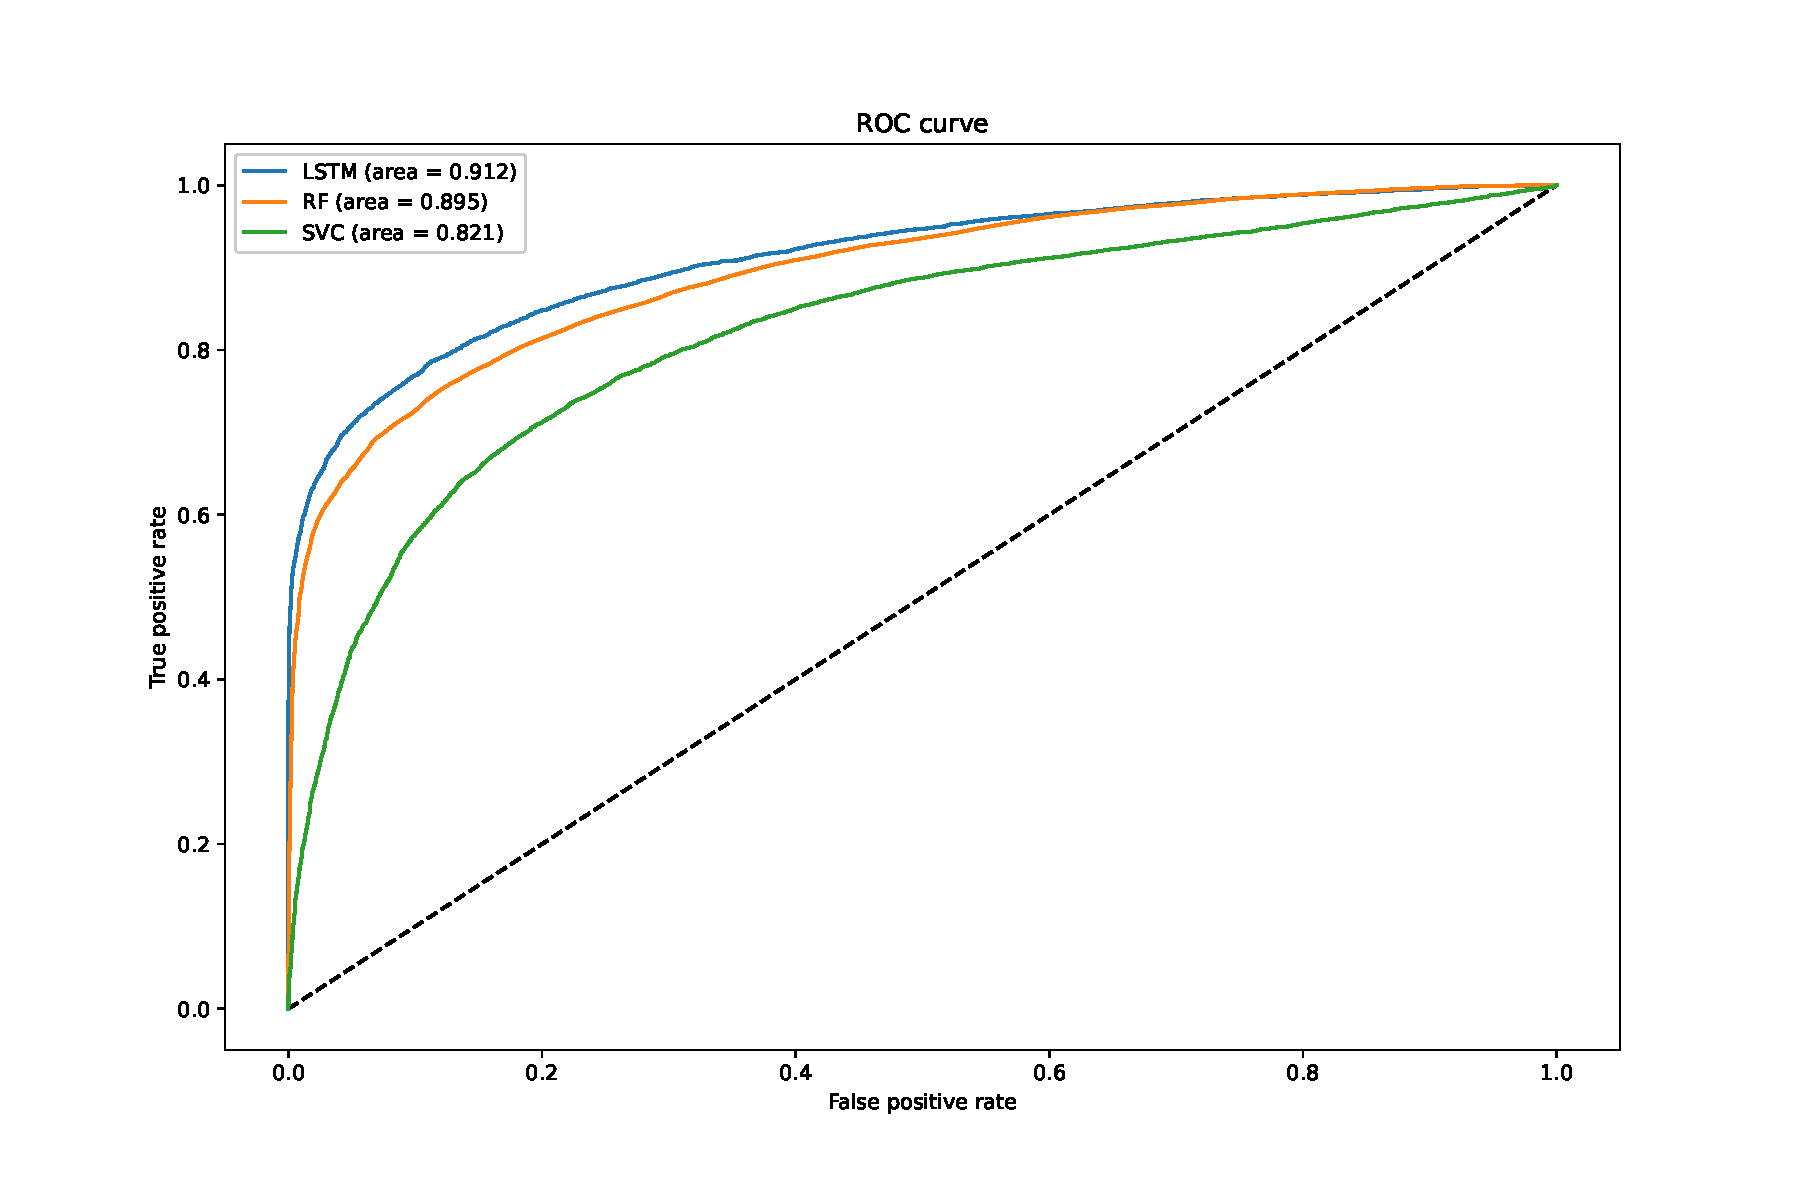
\includegraphics[width=\textwidth]{figs/roc-phish-2017-lstm-rf-svc.pdf}\\PhishTank
	\end{minipage}
	\begin{minipage}[b]{0.45\textwidth}
	\centering
	\label{malware_compare}
	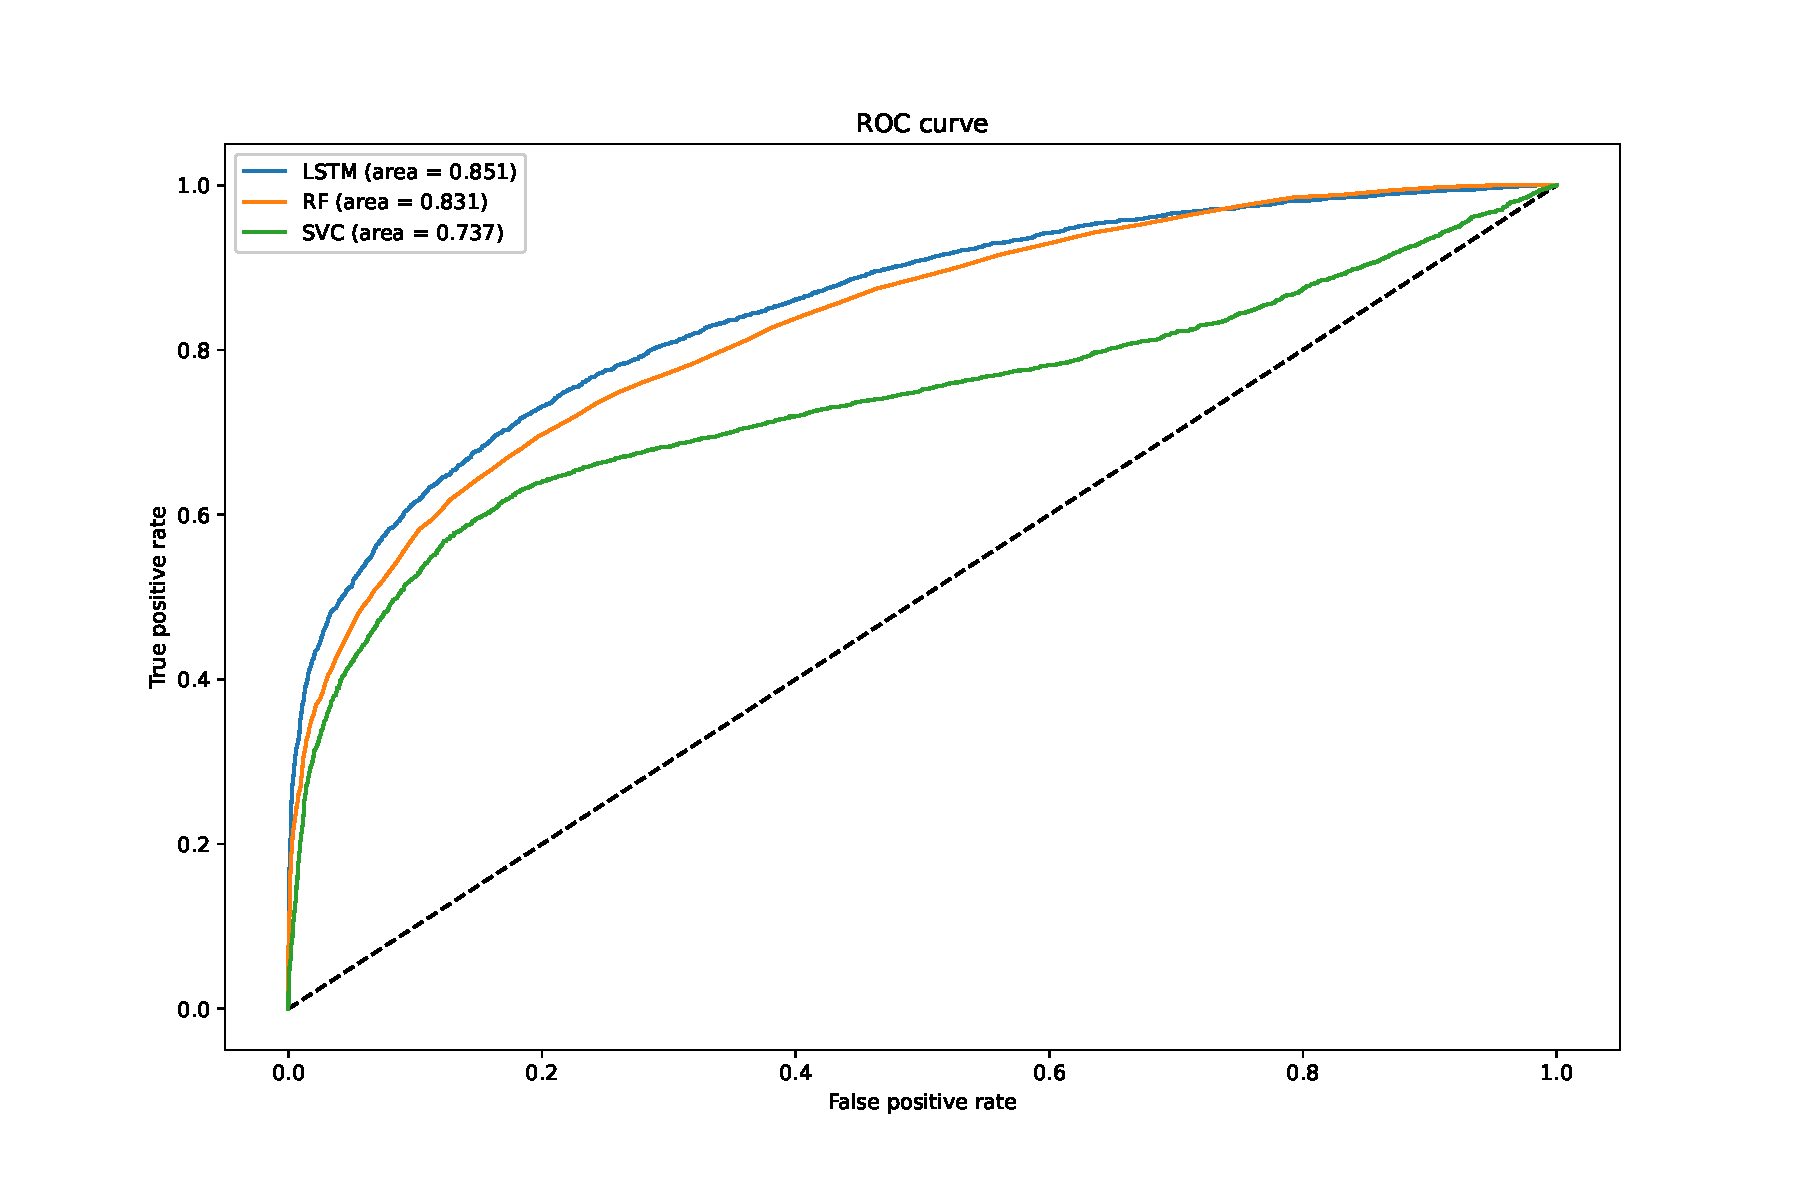
\includegraphics[width=\textwidth]{figs/roc-malware-lstm-rf-svc.pdf}\\Malware
	\end{minipage}
\end{figure}

For Shallalist, precision, recall, and f1-score are .76, .76, and .76, respectively (see Table ~\ref{tab:shalla_model}). There is a sizable variation in recall across categories. For instance, recall is .93 for pornography and just .35 for fortune-telling. Overall, however, Random Forest and SVC do much worse here with f1-scores of .62 and .04, respectively. (We had to truncate the SVC model after 500 iterations as even after running it for two days, the model never converged.) Figure \ref{shalla_lstm_rf_svm} clearly shows the performance advantage of the LSTM model over the other two models.

\begin{figure}[!htb]
\centering
\caption{Shallalist Model Performance}\label{shalla_lstm_rf_svm}
	\begin{minipage}[b]{0.3\textwidth}
	\centering
	\label{toulouse_lstm}
	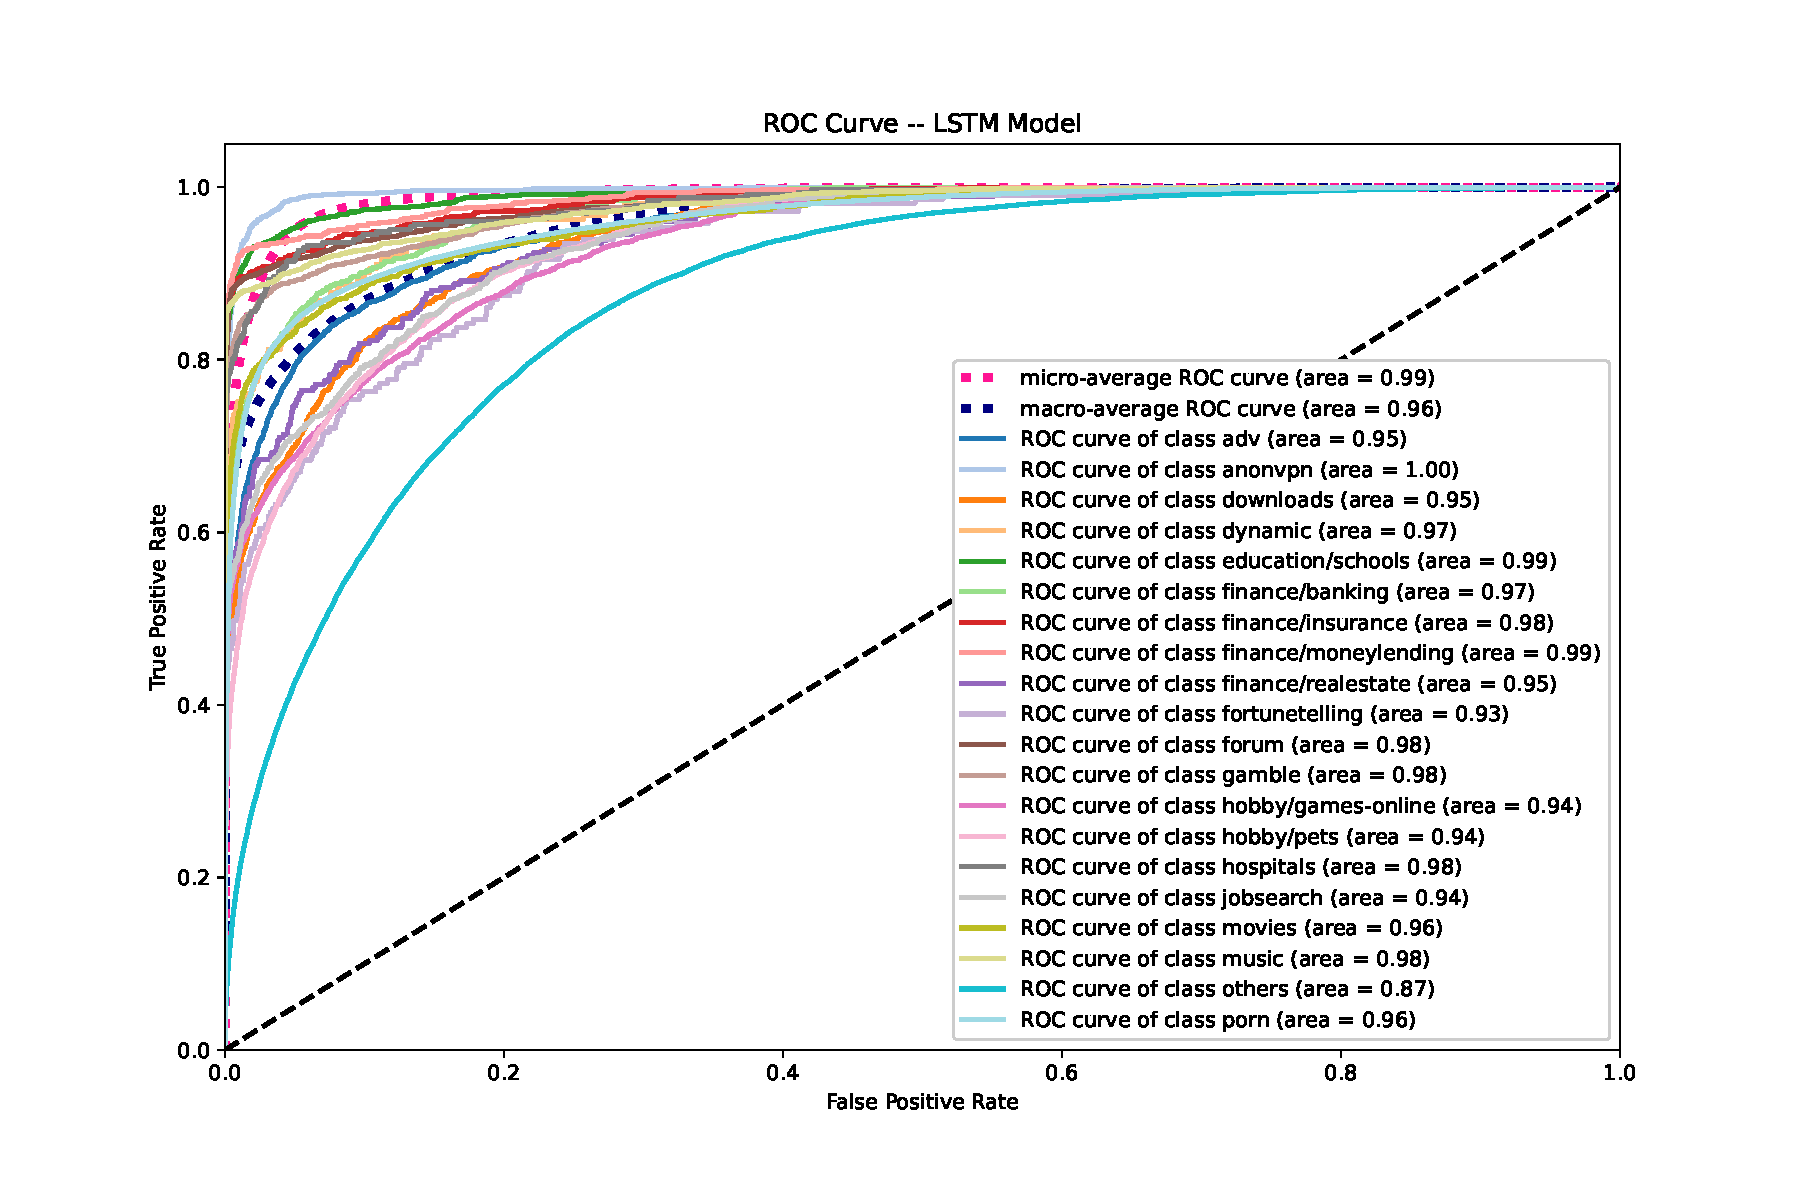
\includegraphics[width=\textwidth]{figs/roc-shalla-2017-lstm.pdf}\\LSTM
	\end{minipage}
	\begin{minipage}[b]{0.3\textwidth}
	\centering
	\label{toulouse_rf}
	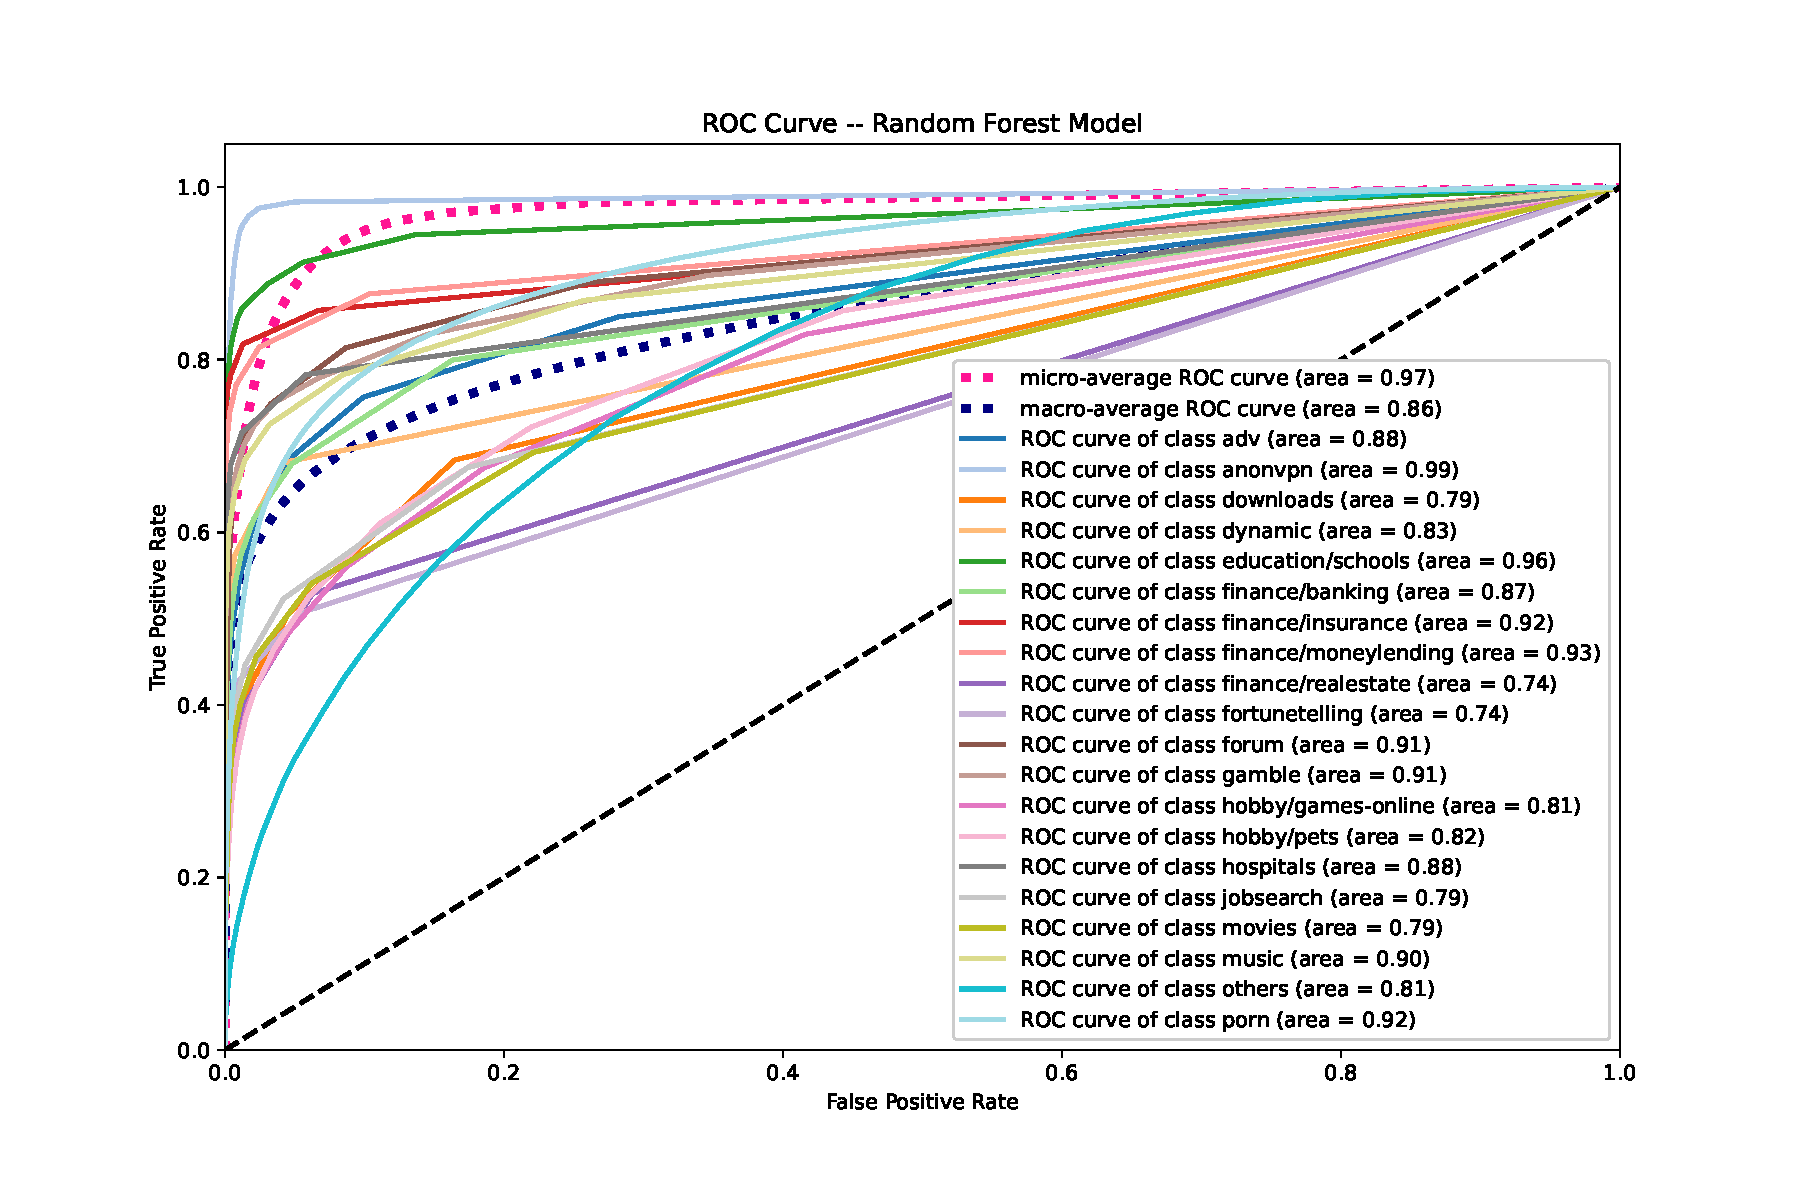
\includegraphics[width=\textwidth]{figs/roc-shalla-2017-rf.pdf}\\Random Forest
	\end{minipage}
	\begin{minipage}[b]{0.3\textwidth}
	\centering
	\label{toulouse_rf}
	\includegraphics[width=\textwidth]{figs/shalla_svm.png}\\SVC
	\end{minipage}
\end{figure}

For the Toulouse data, with much fewer categories than Shallalist, things look vastly better (see Table ~\ref{tab:toulouse_model}). The average accuracy, recall, and f1-score are .95, .96, and .95, respectively. A closer inspection, however, suggests that the gains are largely driven by the largest category, which is adult content. In all, we can learn an excellent adult domain classifier. Once again, SVC and Random Forest perform much worse (see Figure ~\ref{toulouse_lstm_rf_svm}).

\begin{figure}[!htb]
\centering
\caption{Toulouse Model Performance}\label{toulouse_lstm_rf_svm}
	\begin{minipage}[b]{0.3\textwidth}
	\centering
	\label{toulouse_lstm}
	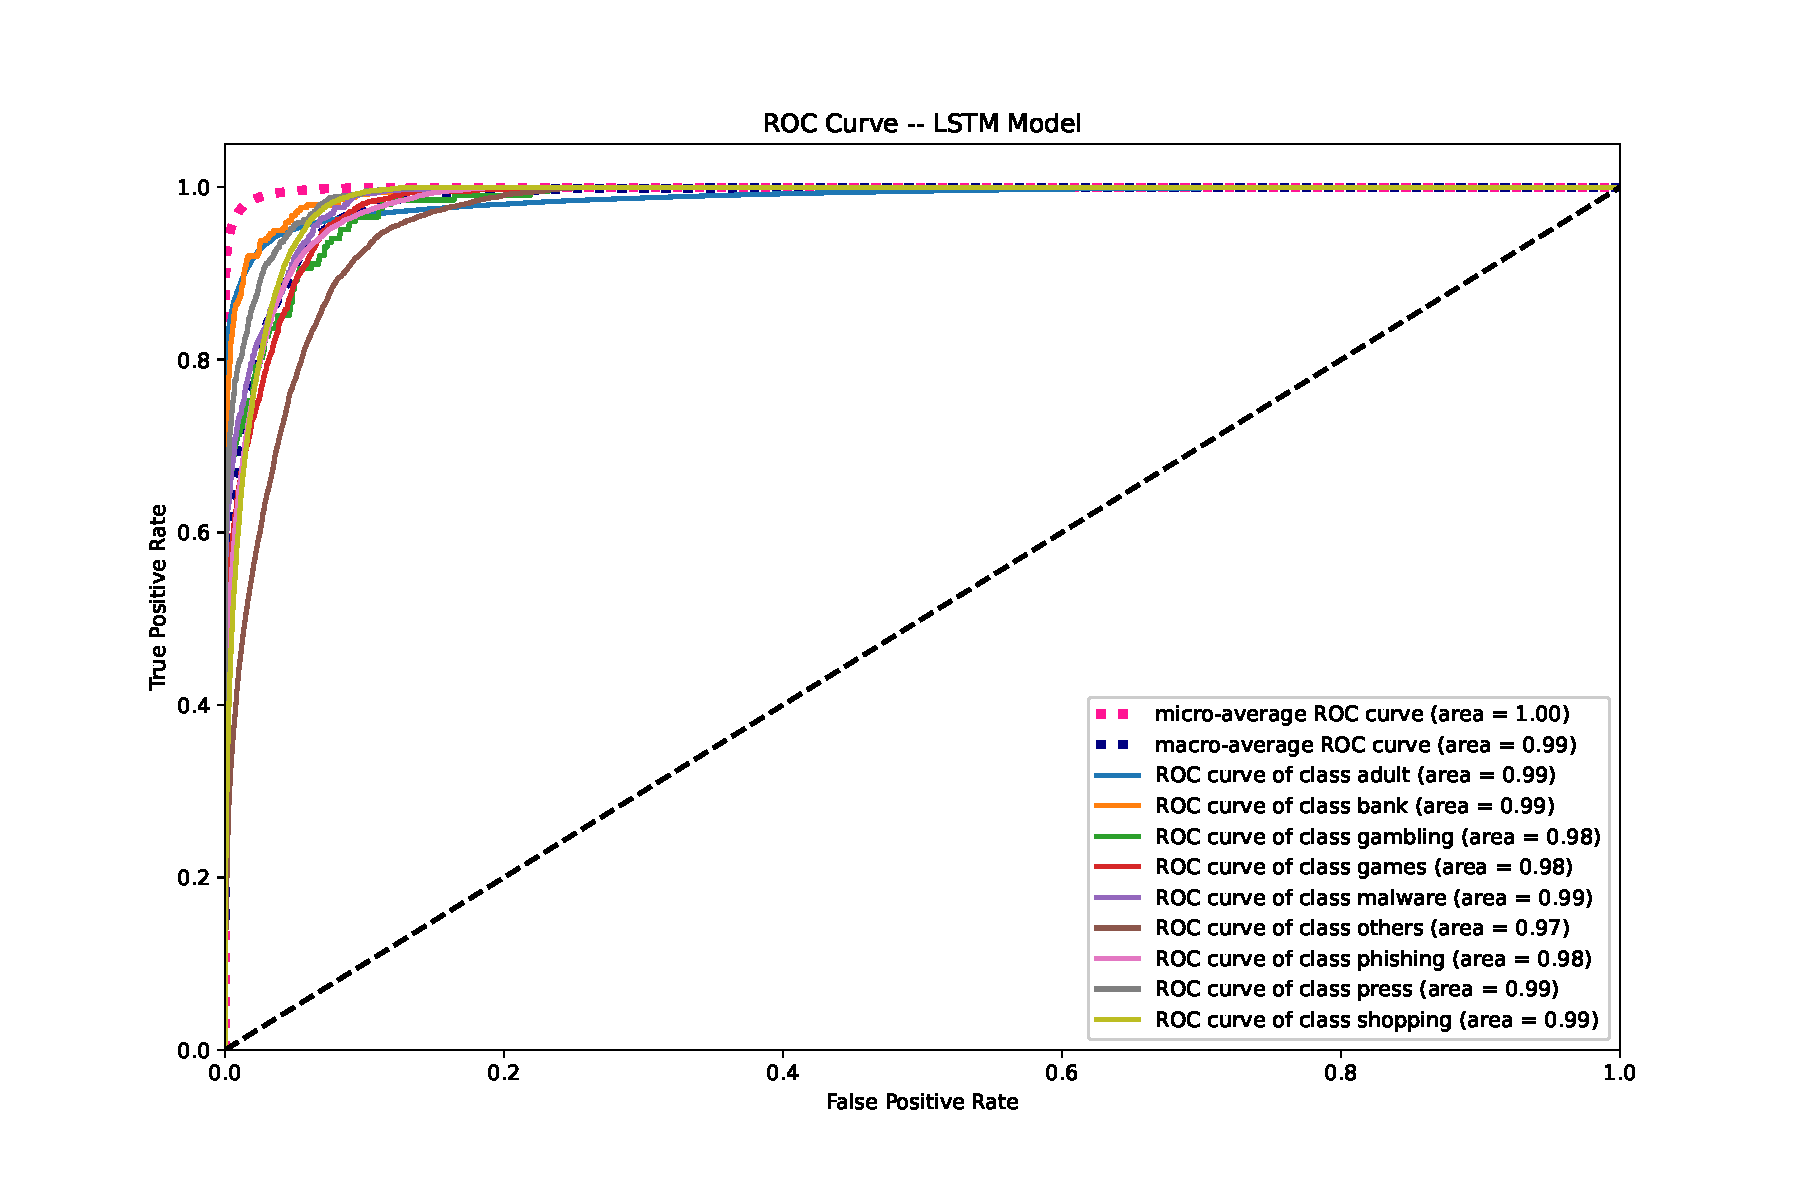
\includegraphics[width=\textwidth]{figs/roc-toulouse-2017-lstm.pdf}\\LSTM
	\end{minipage}
	\begin{minipage}[b]{0.3\textwidth}
	\centering
	\label{toulouse_rf}
	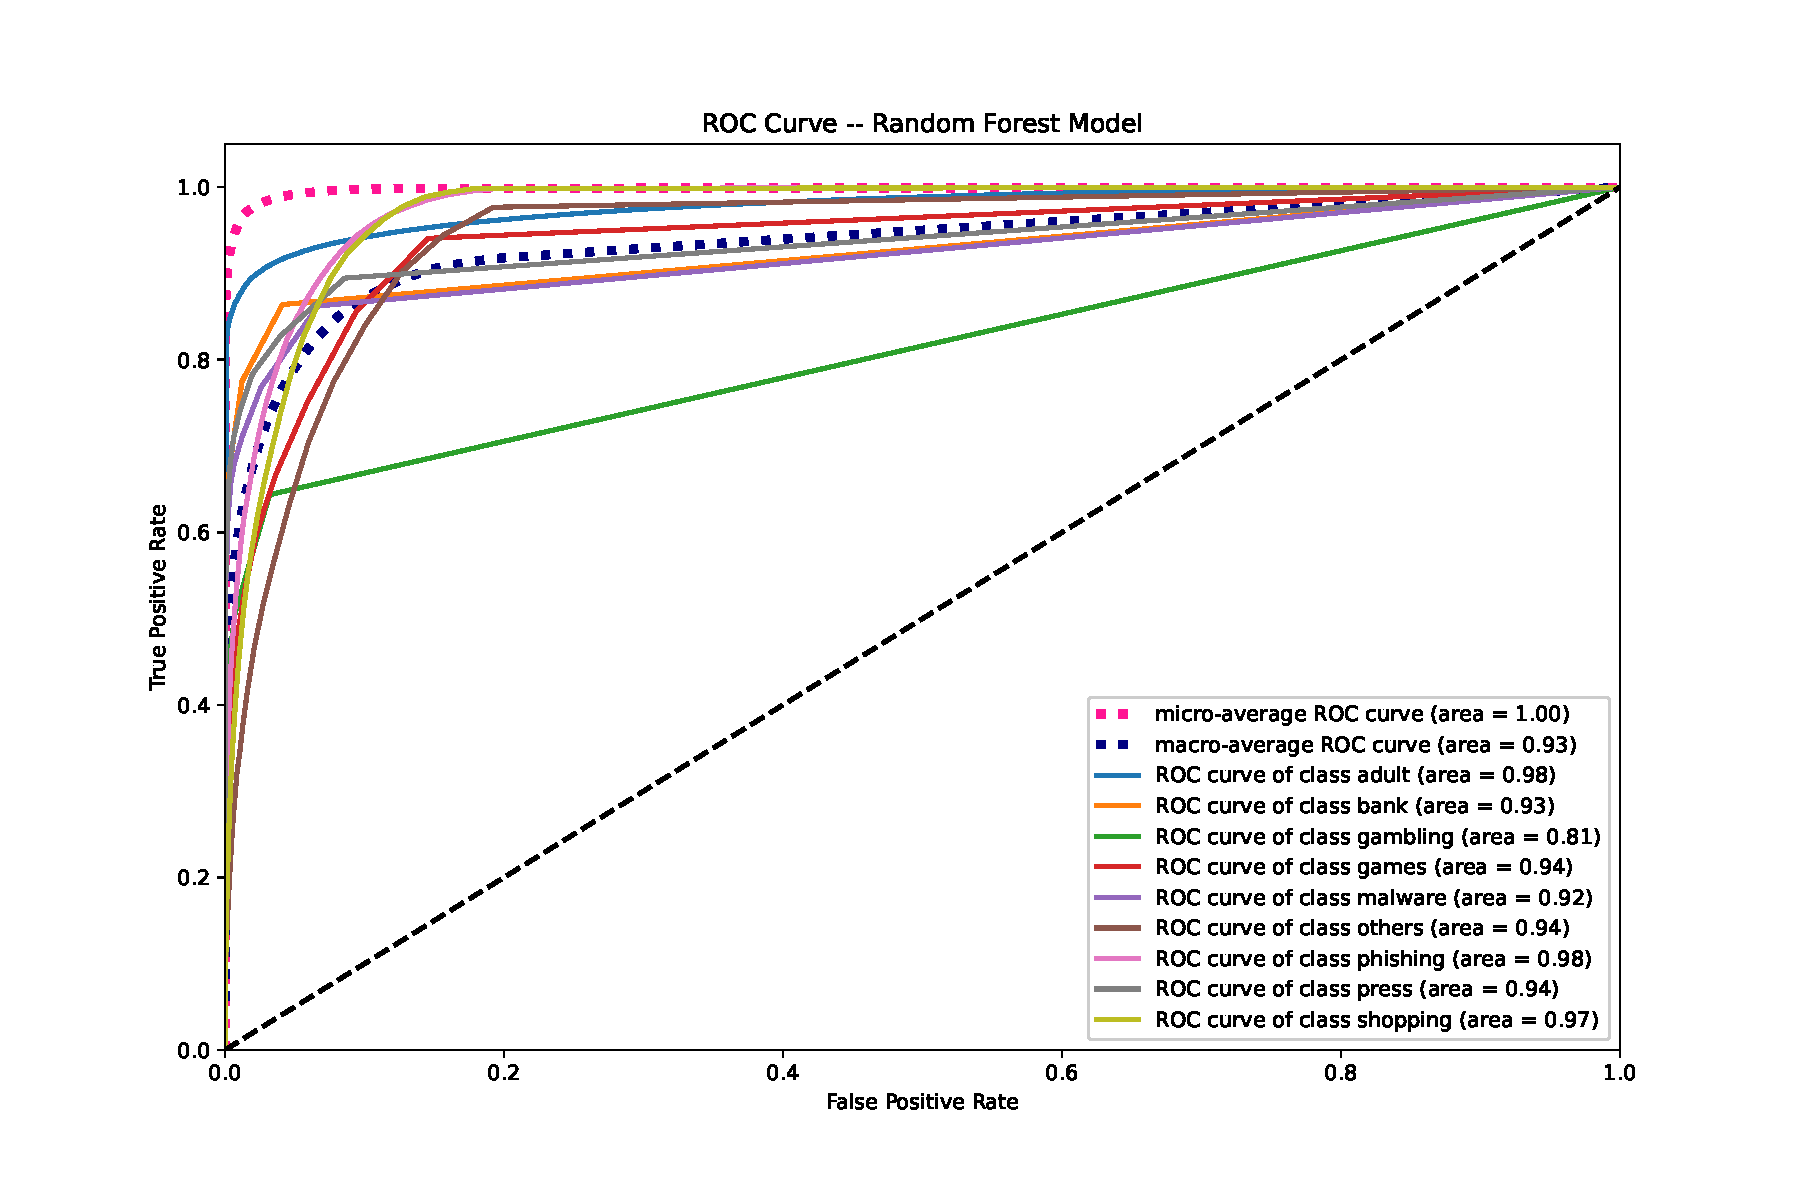
\includegraphics[width=\textwidth]{figs/roc-toulouse-2017-rf.pdf}\\Random Forest
	\end{minipage}
	\begin{minipage}[b]{0.3\textwidth}
	\centering
	\label{toulouse_rf}
	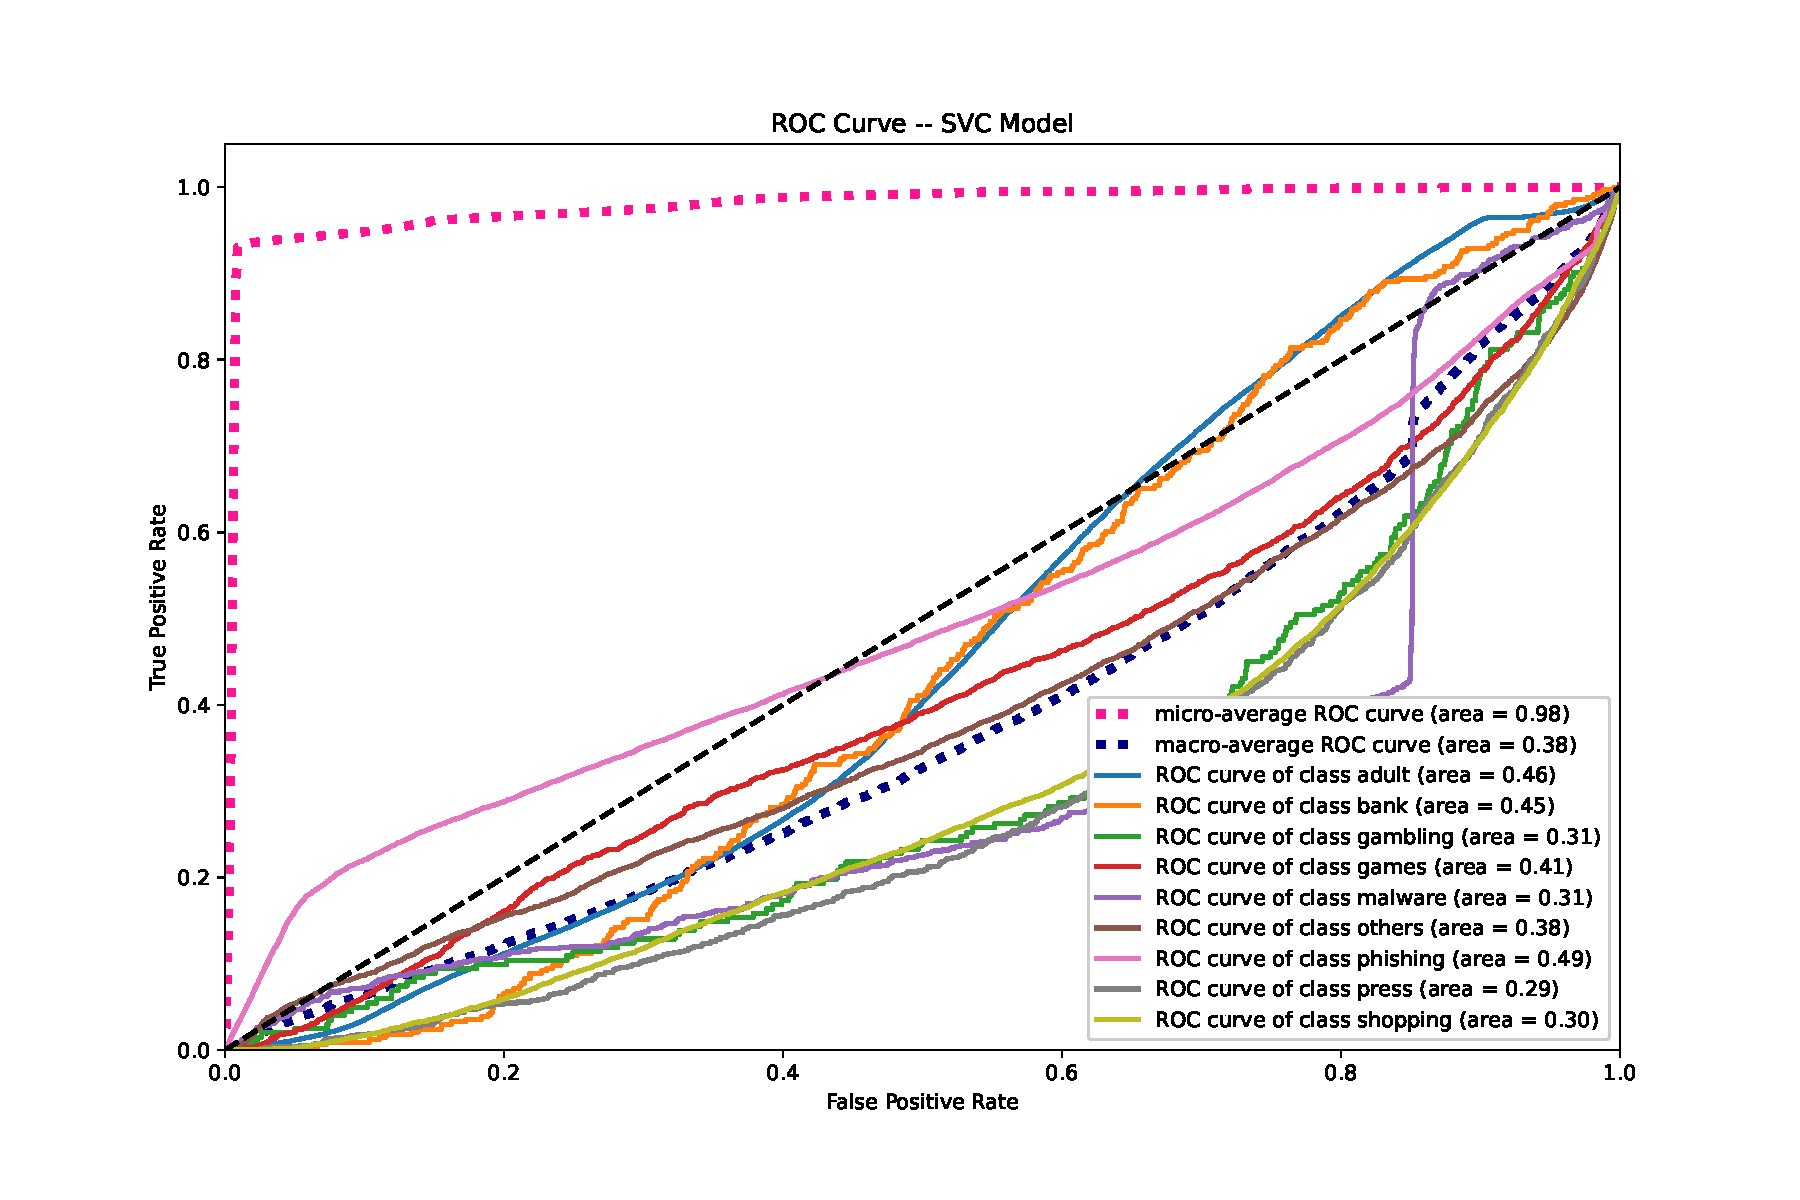
\includegraphics[width=\textwidth]{figs/roc-toulouse-2017-svc.pdf}\\SVC
	\end{minipage}
\end{figure}

\section{Application}
We use the models developed in the paper to shed light on two important questions. First, are disadvantaged people are more at risk online? In particular, do racial minorities, the less well-educated, and poor visit websites that host harmful content more frequently than their respective counterparts---those who belong to the majority racial group, the better educated, the higher income. Second, there is concern that consumption of adult content negatively affects attitudes and behavior toward women \citep{hald2010pornography}. We shed light on the issue by measuring the extent to which people consume adult content, and how it varies by education and age.

We answer the questions using data from Comscore. Comscore maintains an online panel of approximately 100,000 users. It collects anonymous browsing data on a machine in exchange for small perks. Comscore distributes anonymized domain-level data at the machine level along with some household-level characteristics to researchers. We capitalize on the data here.

Aside from Hawthorne effect, there are at least three problems with the data:
\begin{itemize}
  \item \textbf{Domain level data}: Going to \url{http://nytimes.com} is not the same as reading political news. And measurement error varies by the kind of person. For instance, say we label \url{http://nytimes.com} as political news. For a political junkie, the measurement error for that class label may be zero. For a political teetotaler, it may be 100\%. More generally, domain-level data mean that we count all visits to a domain the same. Some domains host heterogeneous content. And people may self-select into 'off-label' content.

  \item \textbf{Machine level data}: these days people browse the Internet on multiple machines \citep{deloitte2019}. And increasingly, the primary machine they browse Internet on is a tablet or a phone. We do not have data on what proportion of browsing a person does on the machine from which the data is being collected and we do know whether the browsing behavior, e.g., what proportion of time is spent on different websites, etc., varies across machines.

  \item \textbf{Household level demographic data}: Where you have more than one person in a household, we cannot cleanly attribute characteristics to a person. For age and education, for instance, Comscore gives the age (education) of the oldest (most educated) person in the household. For income, Comscore gives the household income.
\end{itemize}

Our strategy for answering the questions is roughly the same. We start with Comscore data for a year that is already aggregated at the machine-domain level and has four columns: machine id, domain name, the number of visits to the domain from people using the machine in a year, amount of time (in minutes, we think) spent on the domain by people using the machine. The data are in long-form---as many rows per device as the total number of unique domains they visit in a year.

We left-join this data using the domain name as key with pre-computed data about the kind of content hosted by a domain. We then aggregate these data by type of content (inferred by a particular method), and we sum the visits and time spent by kind of content. We then left join each of these datasets with demographics data using machine id as the key and investigate how the time spent and the number of visits varies by sociodemographic traits.

\subsection{Browsing Data: Concerns and Solutions}
Say you want to measure how often people visit pornographic domains over some period. To measure that, we build a model to predict whether or not a domain hosts pornography. Let's assume that for the chosen classification threshold, the False Positive rate (FP) is 10\%, and the False Negative rate (FN) is 7\%. Here below, we discuss some of the concerns with using uncalibrated scores from such a model and ways to address the issues.

Let's say that we have $n$ users and that we can iterate over them using $i$. Let's denote the total number of unique domains---domains visited by any of the $n$ users at least once during the observation window---by $k$. And let's use $j$ to iterate over the domains. Let's denote the number of visits to domain $j$ by user $i$ by $c_{ij} = {0, 1, 2, ....}$. And let's denote the total number of unique domains a person visits ($\sum (c_{ij} == 1)$) using $t_i$. Lastly, let's denote predicted labels about whether or not each domain hosts pornography by $p$, so we have $p_1, ..., p_j, ... , p_k$.

With the formalization, we can illustrate one point clearly. Say there are 5 domains with $p$: ${1_1, 1_2, 1_3, 1_4, 1_5}$. Let's say user one visits the first three sites once and let's say that user two visits all five sites once. Given 10\% of the predictions are false positives, the total measurement error in user one's score $= 3 * .10$ and the total measurement error in user two's score $= 5 * .10$. The general point is that total false positives increase as a function of predicted $1s$. And the total number of false negative increase as the number of predicted $0s$. More generally, the total error for user $i$ is (in expectation):

\begin{align}
\label{eq:net_error}
    \sum_1^k c_{ij} * (p_j == 1) * (FP) - c_{ij} * (p_j == 0) * (FN)
\end{align}

Formalizing clarifies three things. First, the net error is a function of $FP - FN$. Second, even when the share of visits to pornographic domains is the same, the larger the number of domains ($t_i$) a person visits, the larger the error in their score (total number of visits to pornographic domains). Third, when $c_{ij}$ are right-skewed, e.g., browsing data, errors in the right tail can be very costly. Concretely, misclassifying domains that people visit a lot can be super expensive---it may even change inferences wholesale.

One way to speak to the first two issues is to use different probability cutoffs for classification. Different probability cutoffs generate different $FN$ and $FP$ rates and allow us to bound inferences. Another way (and the one we take here) is to calibrate the probabilities so that they reflect the actual likelihood of a true positive. (Calibration means setting FP to FN.)

The third point cuts deeper. To address the issue, one could tweak the cost function of the domain level model such that the cost of each error is proportional to usage. But given the skew, it would put a lot of weight on the features of too few domains. And that would likely degrade model performance. A better, simpler solution may be to use the labels from the dataset used in training. Labeled datasets like the Shallalist cover a vast majority of the heavily visited domains. And using labels from the training set means saves us from the most costly errors.  Doing so also means that we won't be introducing (adding to) measurement error for cases where we have little measurement error.

We can further reduce errors by downloading the top 1M domains from Alexa, taking the difference from the original labeled dataset, and for the remaining domains that are also in the universe of domains you are analyzing, use some reputable web service to get the category of content hosted by the domain. We adopt this technique when looking at pornographic domains.

Yet another way to make analysis robust to skew is to winsorize usage within users. Winsorization reduces the impact of miclassified heavily visited domains. But the downside is that it adds bias to the usage data.

\subsection{Bad Domains}
Using Comscore data from 2016 and predictions from our LSTM Malware, 2017 PhishTank, and Toulouse models, we assessed whether African Americans, the less educated, and older people are more at risk online.

Somewhat surprisingly, the most educated most frequently visit (spend most time on) phishing/malware websites (see Figure \ref{fig:total_visits_phishing_malware} and Figure \ref{fig:total_time_phishing_malware_educ}). This is consistent with \citep{cor2018pwned}, who find that the educated are hacked more often. Part of the reason why the more educated visit harmful websites more is because they are online more often. When we look at the proportion of time spent on harmful websites, the most educated spend, if anything, slightly less than the less well educated (see \ref{fig:prop_total_time_phishing_malware_educ}).

\begin{figure}[!htb]
\centering
\caption{Number of Visits to Phishing/Malware Domains}\label{fig:total_visits_phishing_malware}
	\begin{minipage}[b]{0.32\textwidth}
	\centering
	\label{fig:total_visits_phishing_malware_educ}
	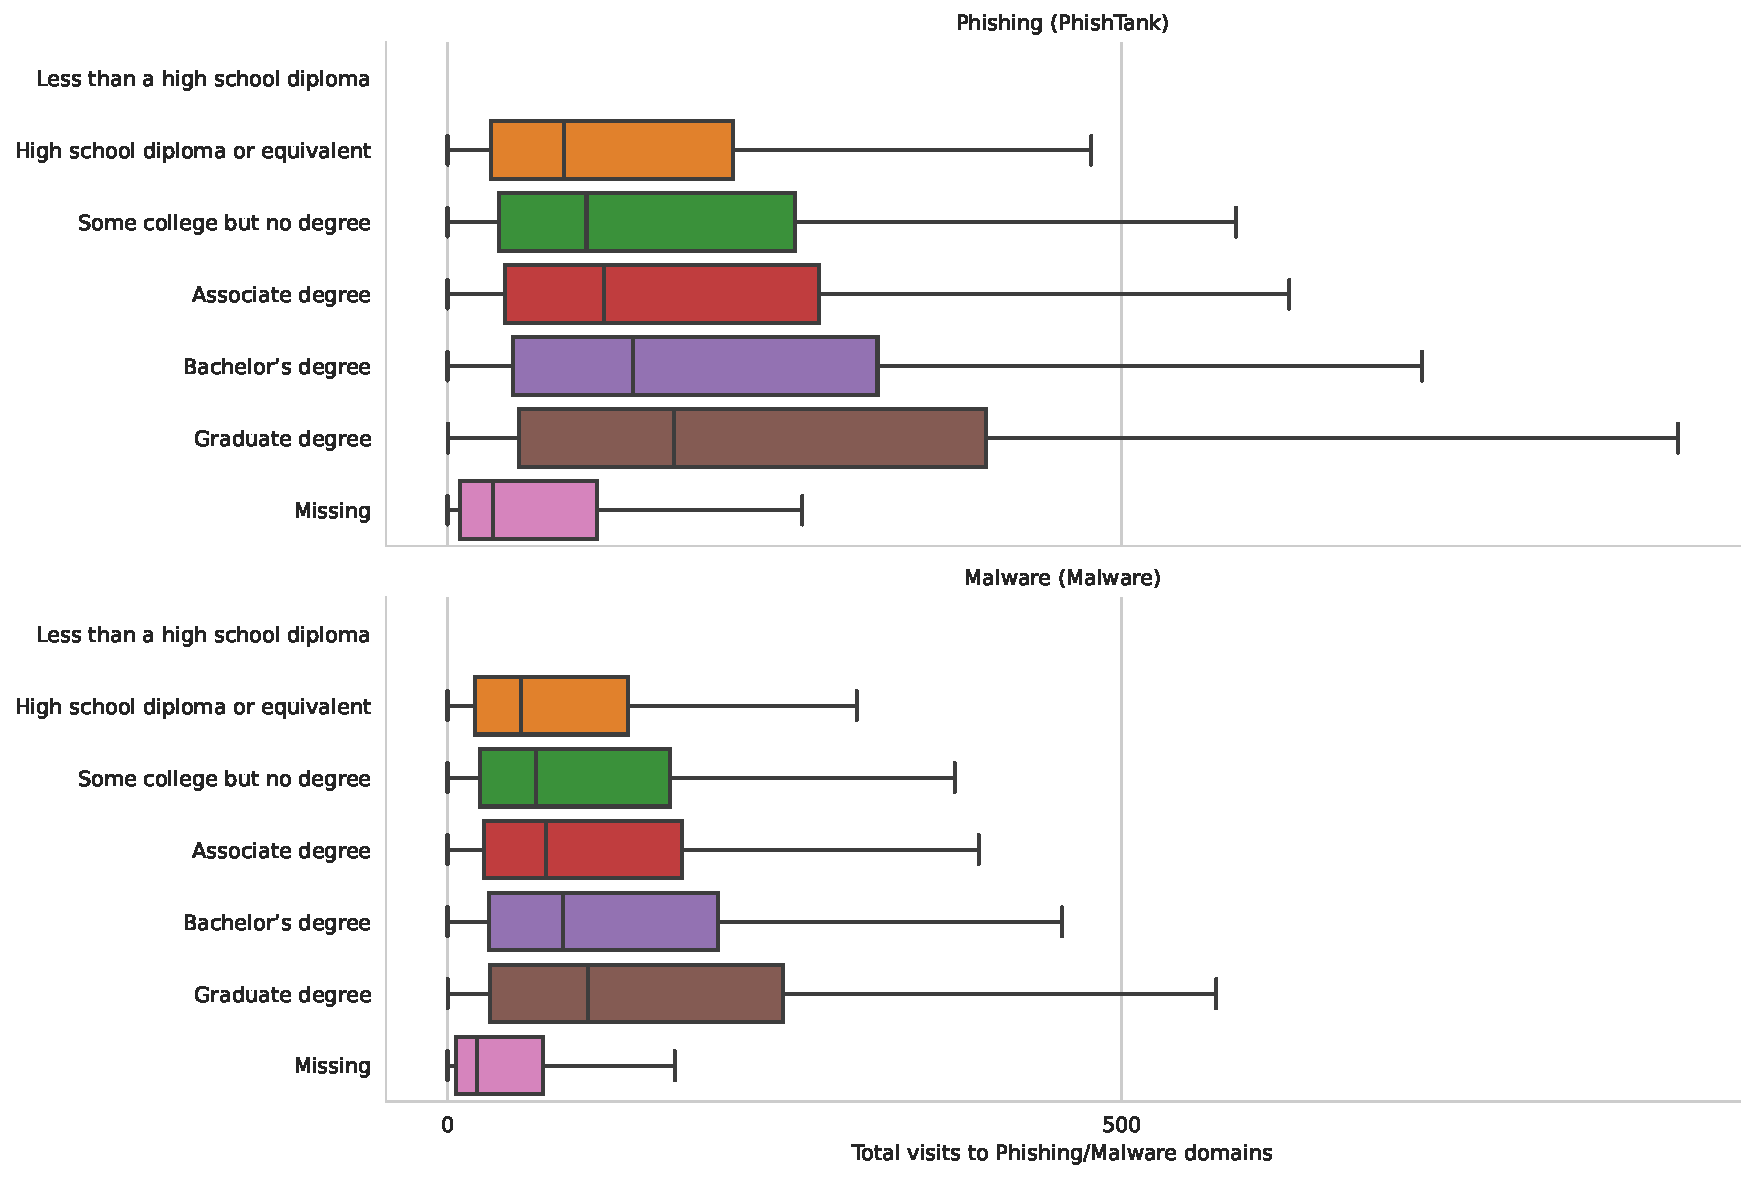
\includegraphics[width=\textwidth]{figs/total_visits_phishing_malware_educ.pdf}\\Education
	\end{minipage}
	\begin{minipage}[b]{0.32\textwidth}
	\centering
	\label{fig:total_visits_phishing_malware_race}
	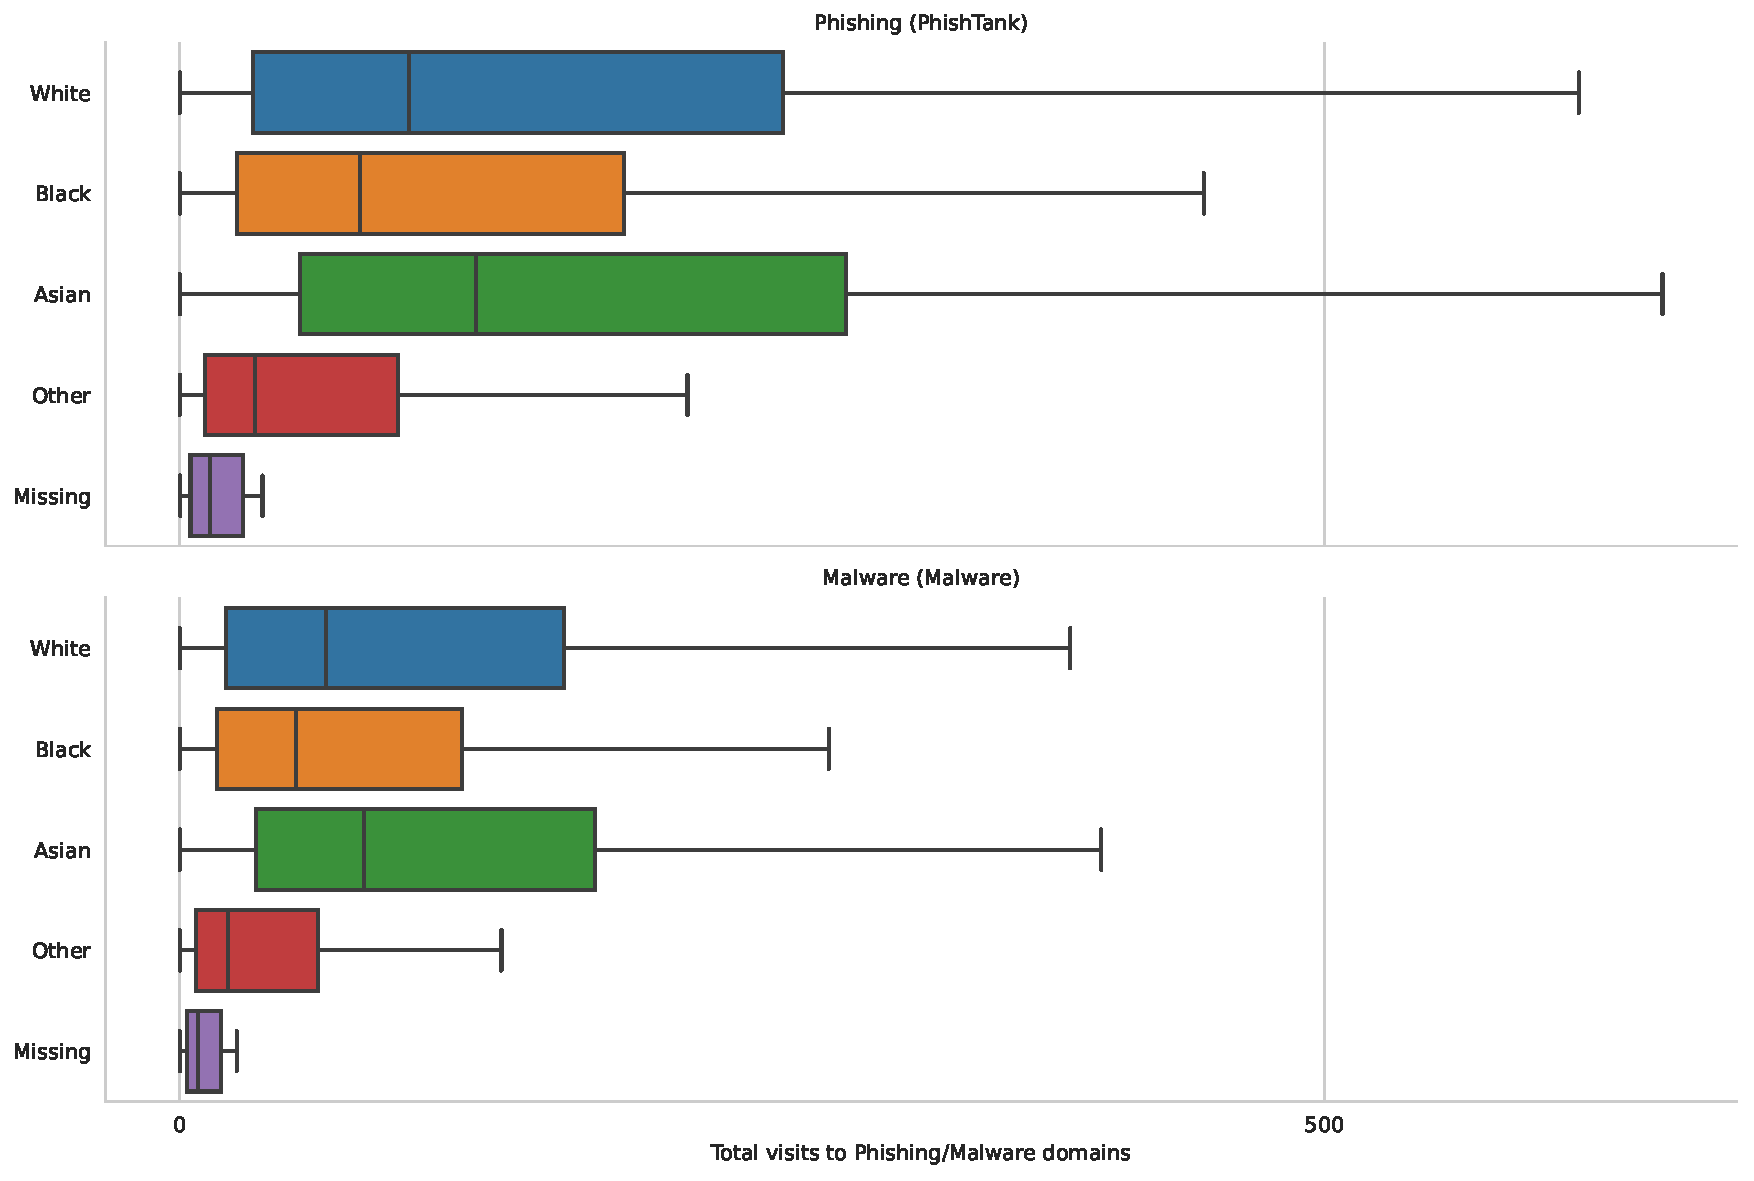
\includegraphics[width=\textwidth]{figs/total_visits_phishing_malware_race.pdf}\\Race
	\end{minipage}
	\begin{minipage}[b]{0.32\textwidth}
	\centering
	\label{fig:total_visits_phishing_malware_age}
	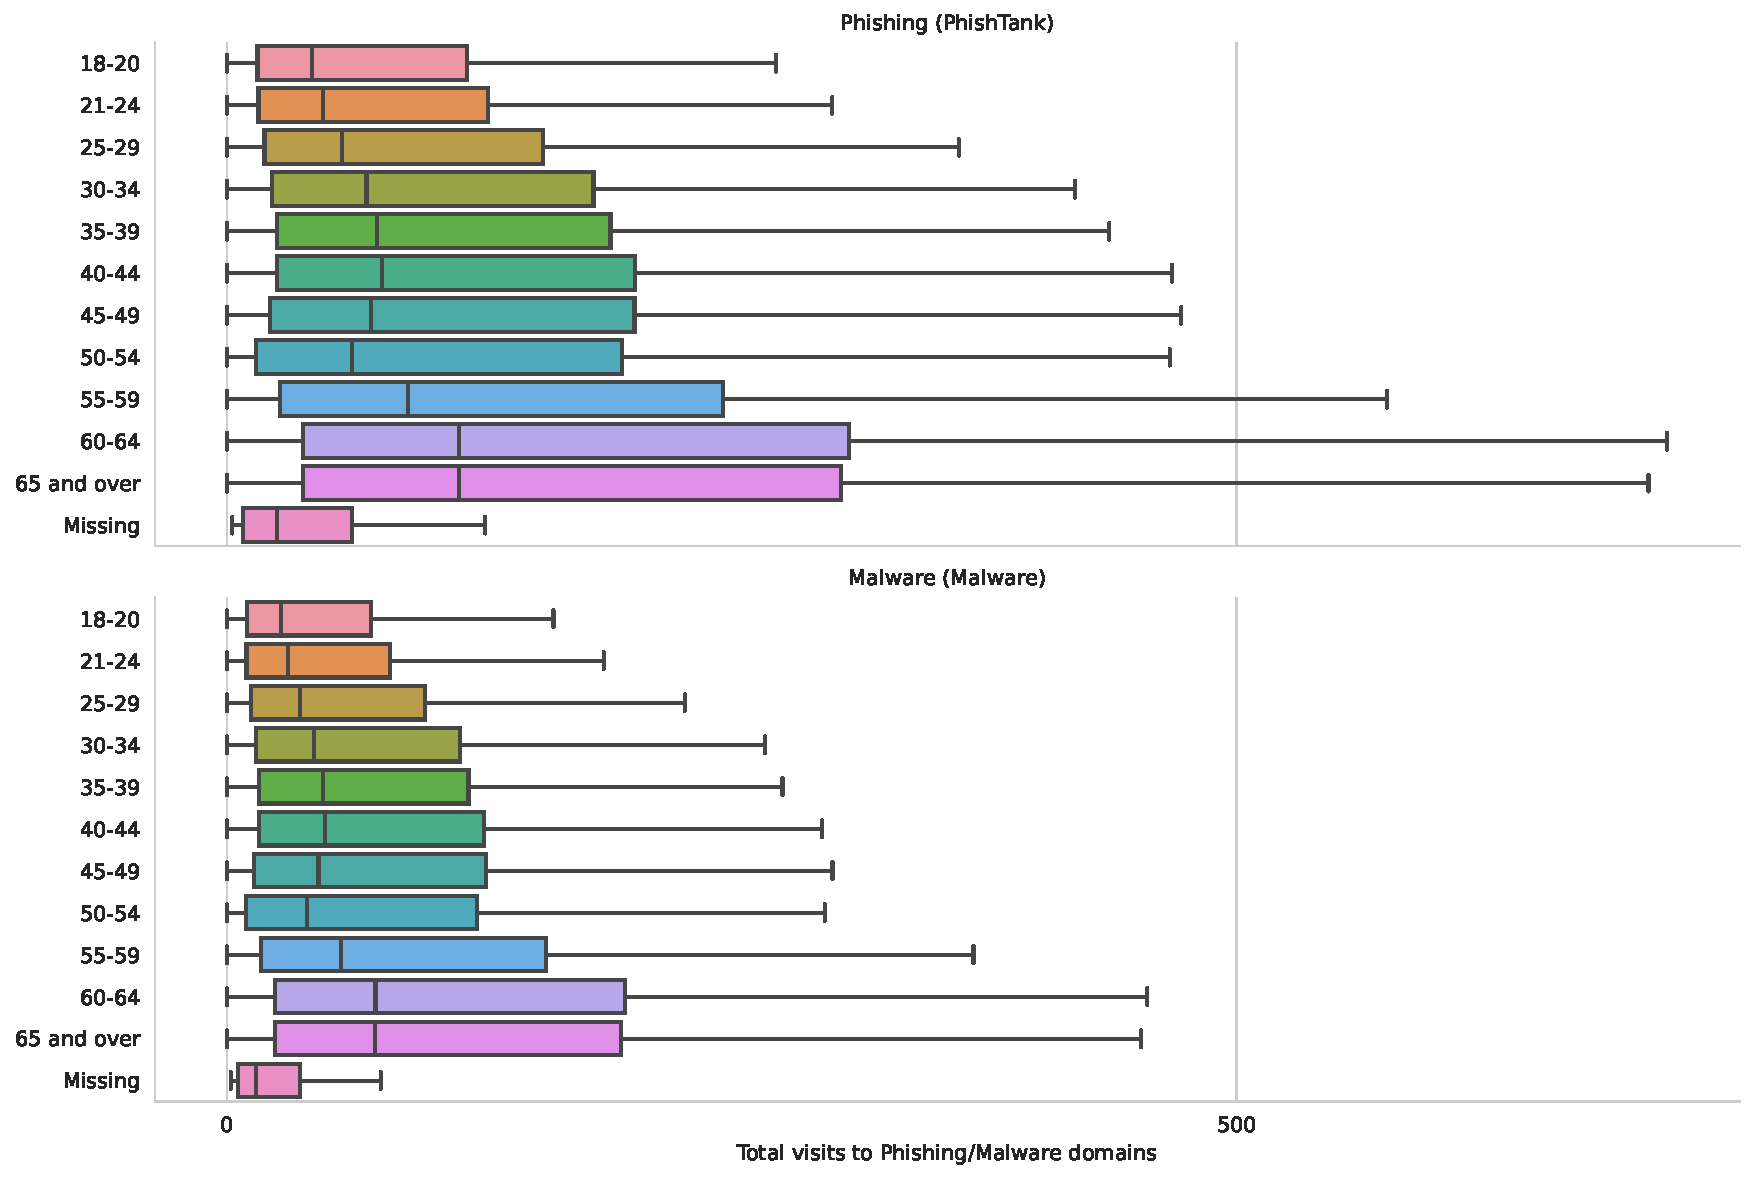
\includegraphics[width=\textwidth]{figs/total_visits_phishing_malware_age.pdf}\\Age
	\end{minipage}
\end{figure}

When we split the sample by race, we find that Asian and White households more frequently visit (spend more time on) malware/phishing websites than other racial groups. Again, it seems part of the reason is that Asians/Whites spend more time online (see Figure \ref{fig:prop_total_visits_phishing_malware_educ}).

Splitting by age, we see that households with older people more frequently visit (spend the most time on) phishing/malware sites. Here there is some evidence that it is because they are choosing worse than younger people, with a slightly larger proportion of their visits going to malware or phishing sites (see Table \ref{fig:prop_total_visits_phishing_malware_age}).

\subsection{Consumption of Pornography}
A consistent pattern emerges across all four versions of our measure: 18--20 visit the pornographic domains the most often, but after that, there is a decline and then a modest upward trend peaking at 40--44 after which the average number of visits roughly monotonically decline (see Figure \ref{fig:total_visits_porn}). You see the same rough pattern in the average time spent as well (see Figure \ref{fig:total_time_porn_age}).

As education levels increase, number of visits to pornographic domains go down (see Figure \ref{fig:total_visits_porn_educ}). (As Figure \ref{fig:total_time_porn_educ} shows, time spent on such sites also decreases.) Households where the most educated person has a graduate degree visit pornographic sites less often and spent less time on them than households where the most educated person has less than an HS diploma.

\begin{figure}[!htb]
\centering
\caption{Number of Visits to Pornographic Domains}\label{fig:total_visits_porn}
	\begin{minipage}[b]{0.47\textwidth}
	\centering
	\label{fig:total_visits_porn_educ}
	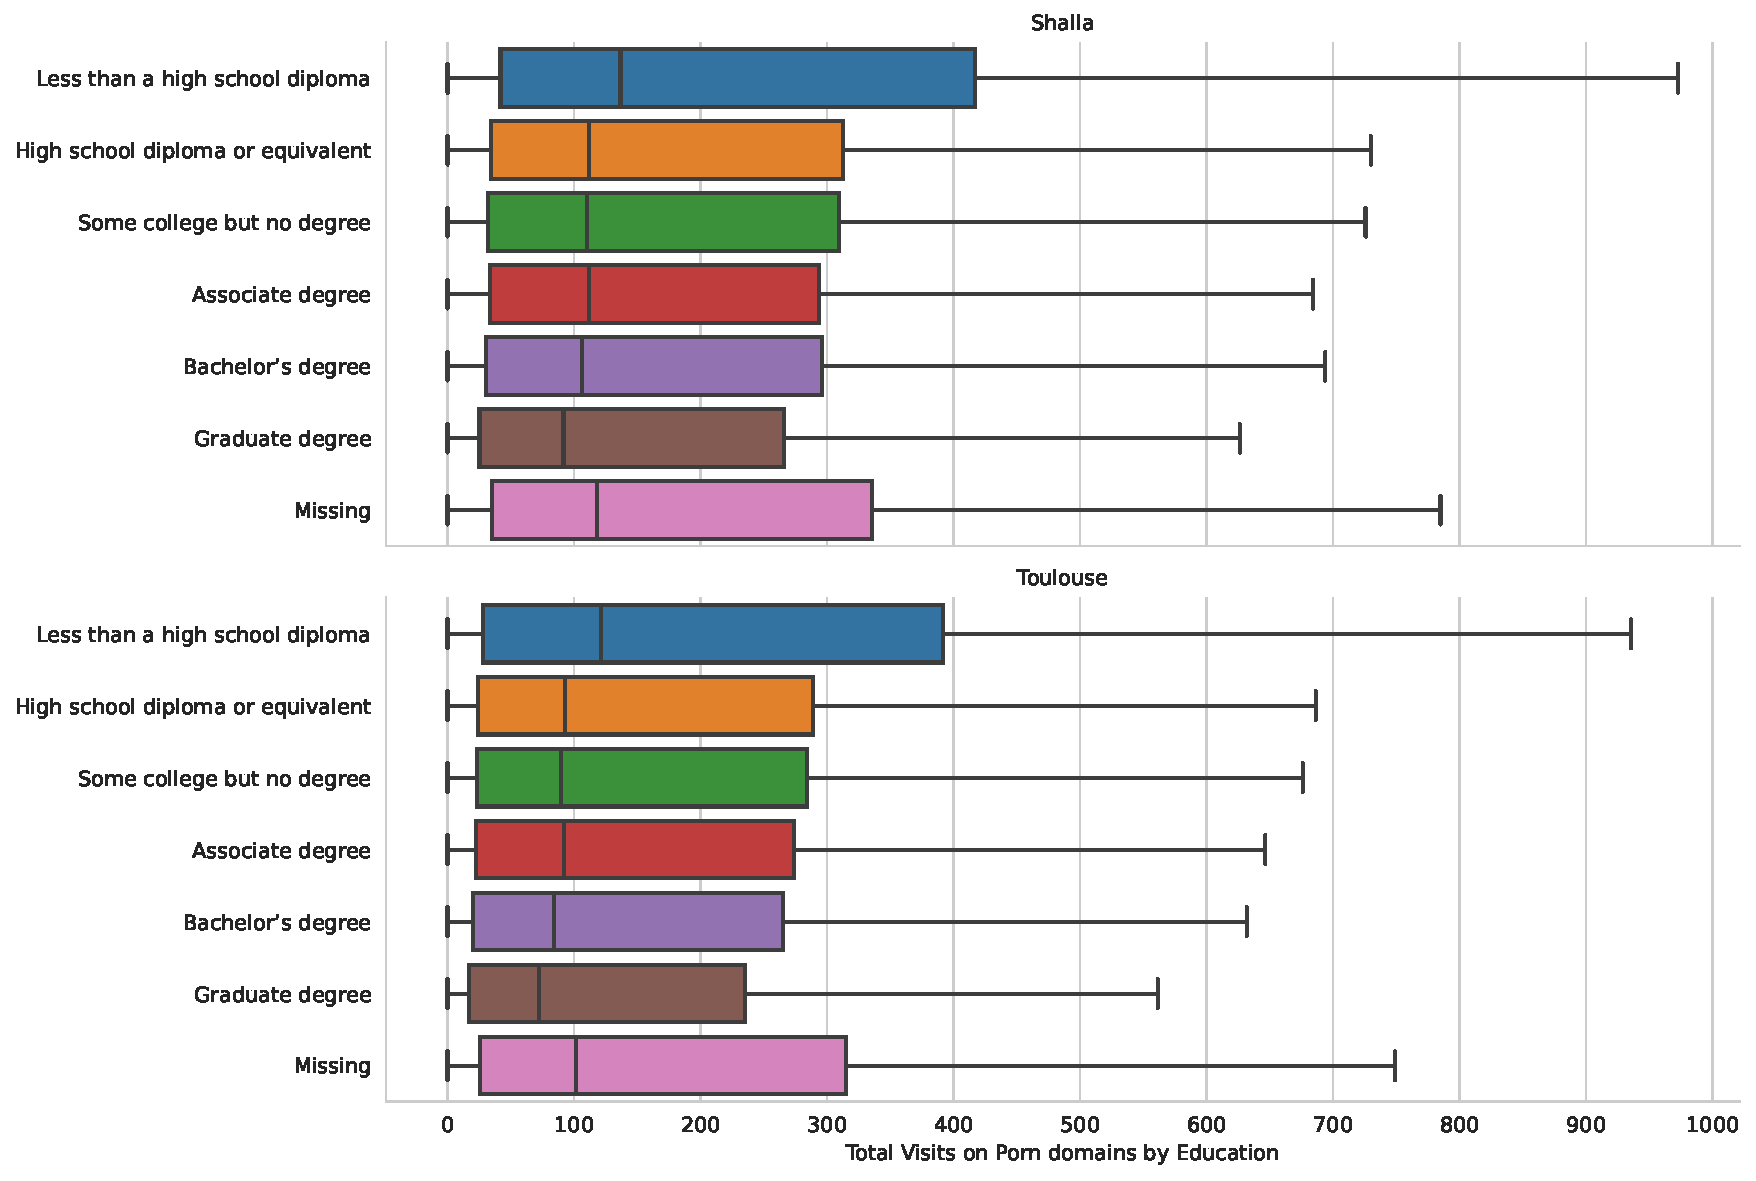
\includegraphics[width=\textwidth]{figs/total_visits_porn_educ.pdf}\\Education
	\end{minipage}
	\begin{minipage}[b]{0.47\textwidth}
	\centering
	\label{fig:total_visits_porn_age}
	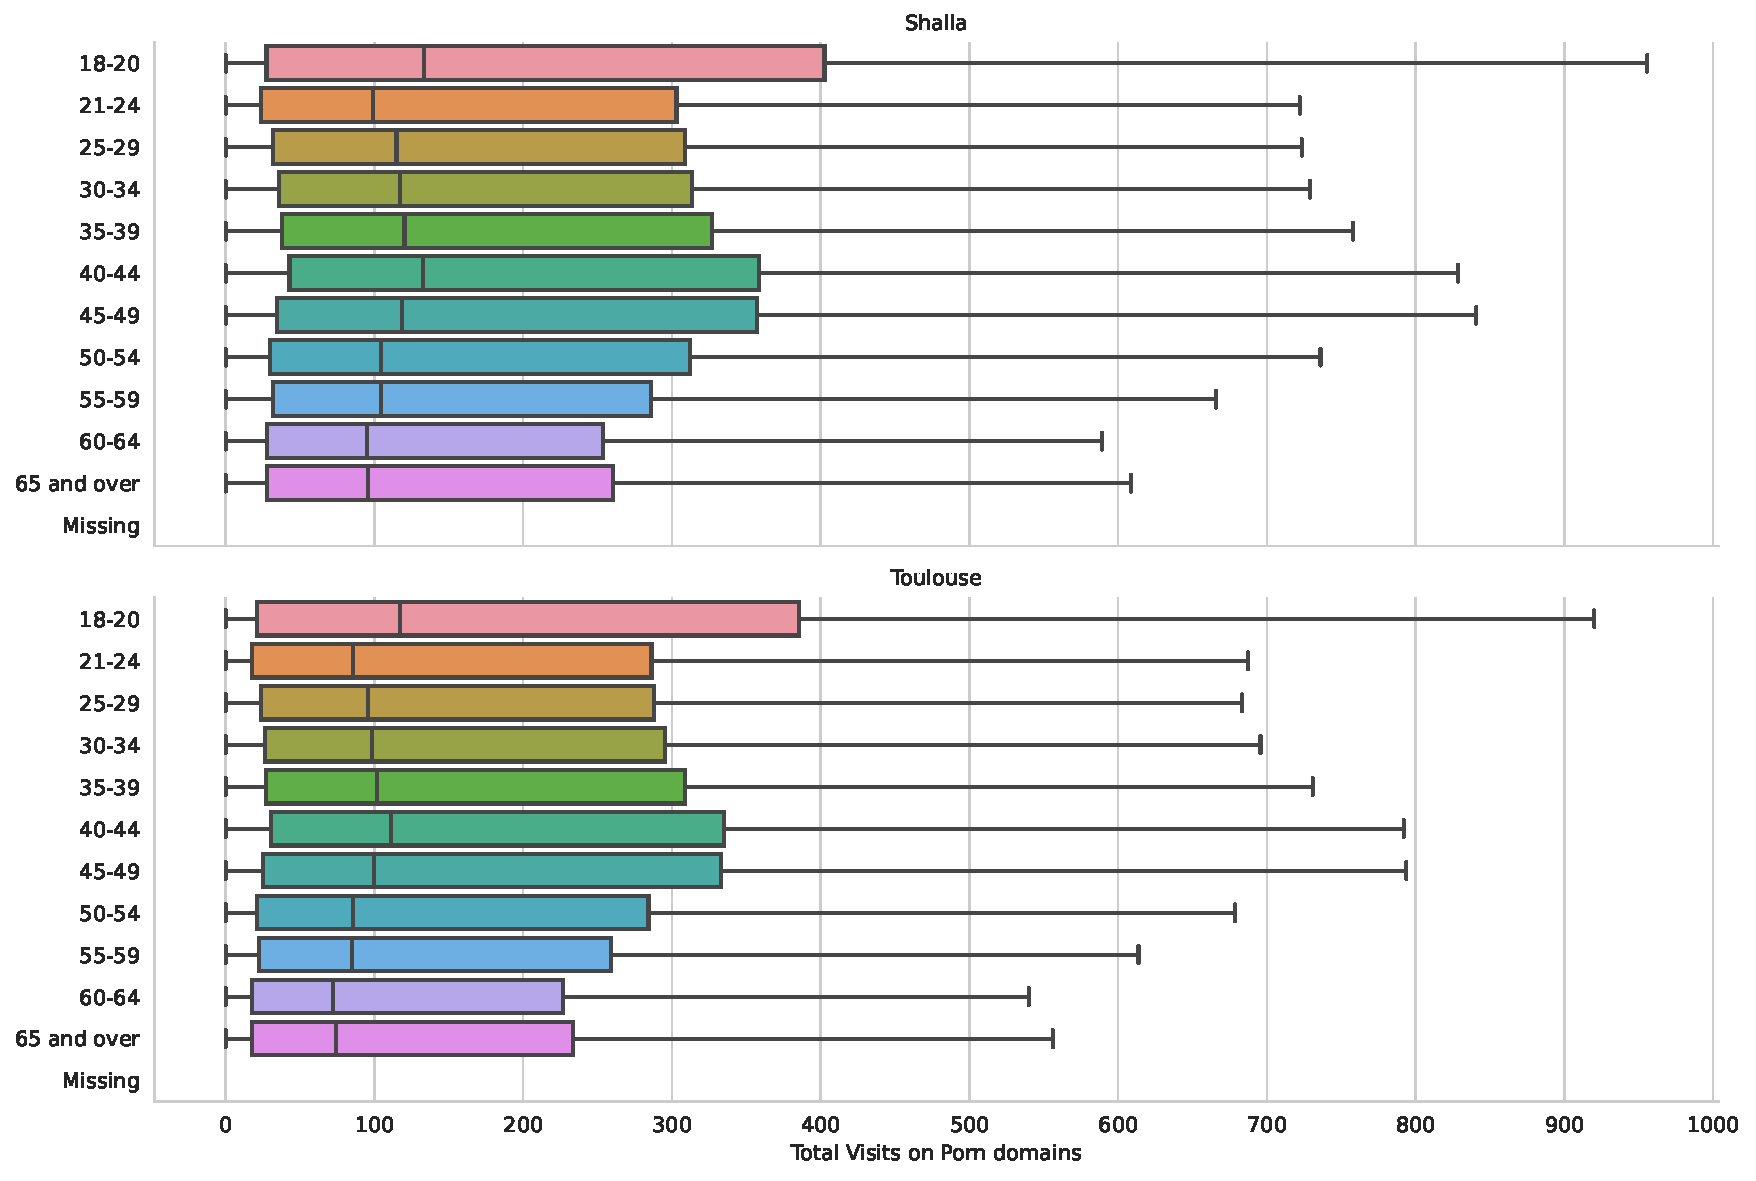
\includegraphics[width=\textwidth]{figs/total_visits_porn_age.pdf}\\Age
	\end{minipage}
\end{figure}

Do we see the patterns because it just captures that certain people spend more time online? To check that, we look at the proportions (see Figures \ref{fig:prop_visits_porn_educ}). The data are clear---as people get older, pornographic websites constitute a smaller share of visits with a roughly monotic decline after 40--44. Splitting by education also shows that the declining trend is a result of people in households where the education level is higher, spending less time on pornographic domains (see Figure \ref{fig:prop_visits_porn_educ}).

\begin{figure}[!htb]
  \centering
  \caption{Proportion of Visits to Pornographic Domains by Education}
	\label{fig:prop_visits_porn_educ}
	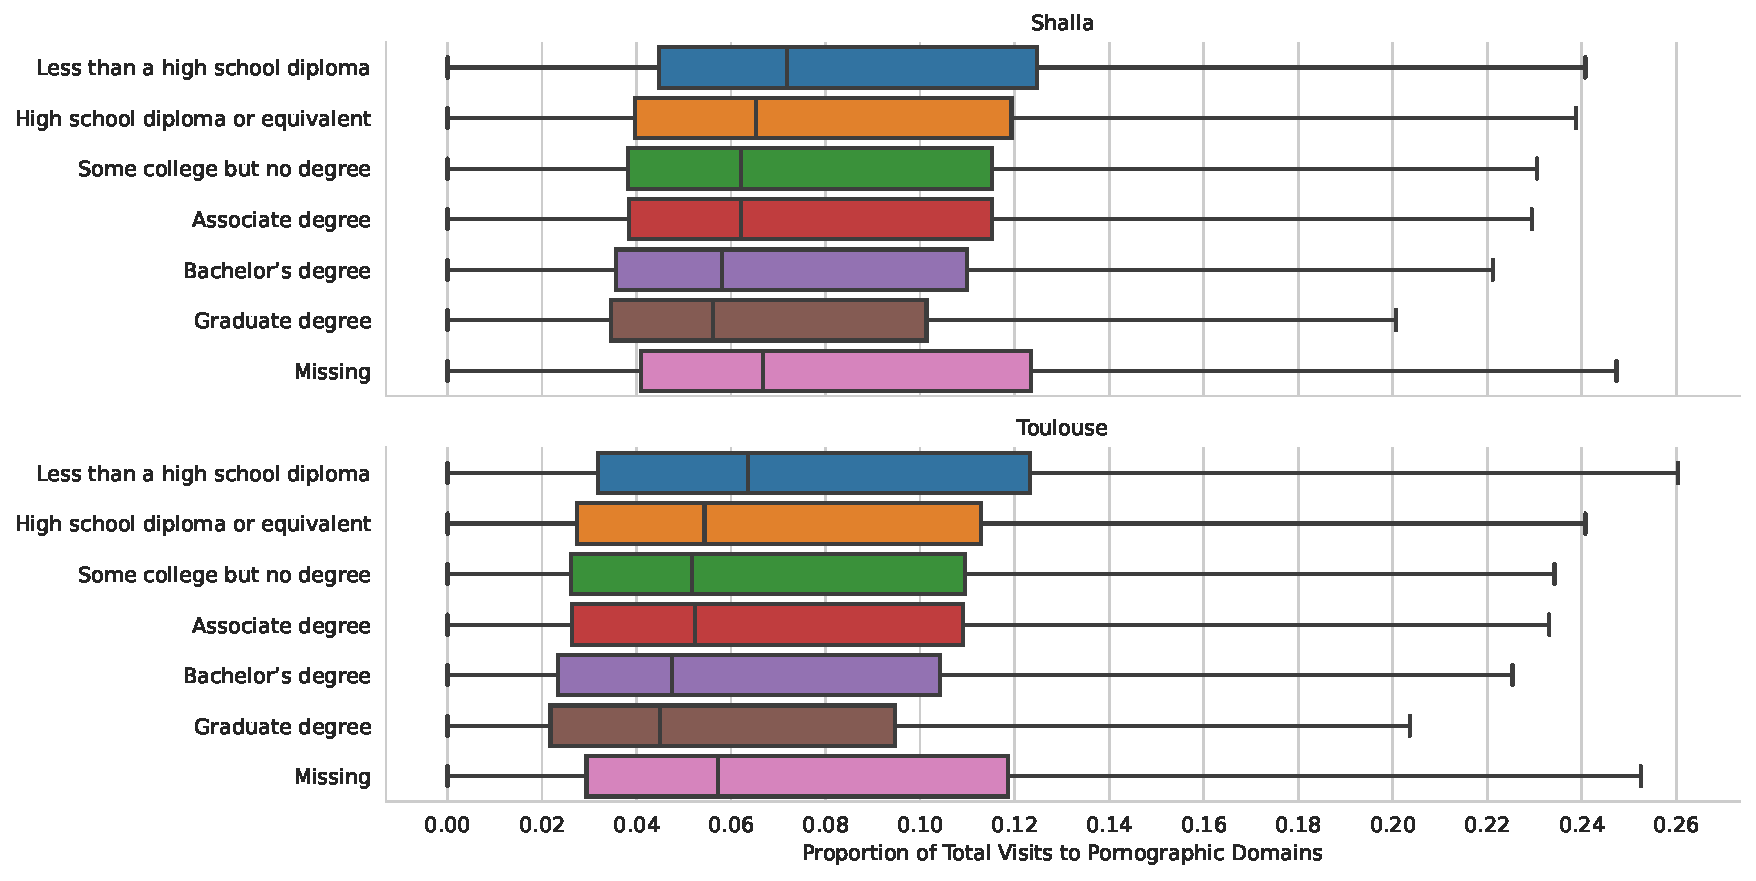
\includegraphics[width=\textwidth]{figs/prop_total_visits_porn_edu.pdf}
\end{figure}

\begin{figure}[!htb]
  \centering
  \caption{Proportion of Visits to Pornographic Domains by Age}
	\label{fig:prop_visits_porn_age}
	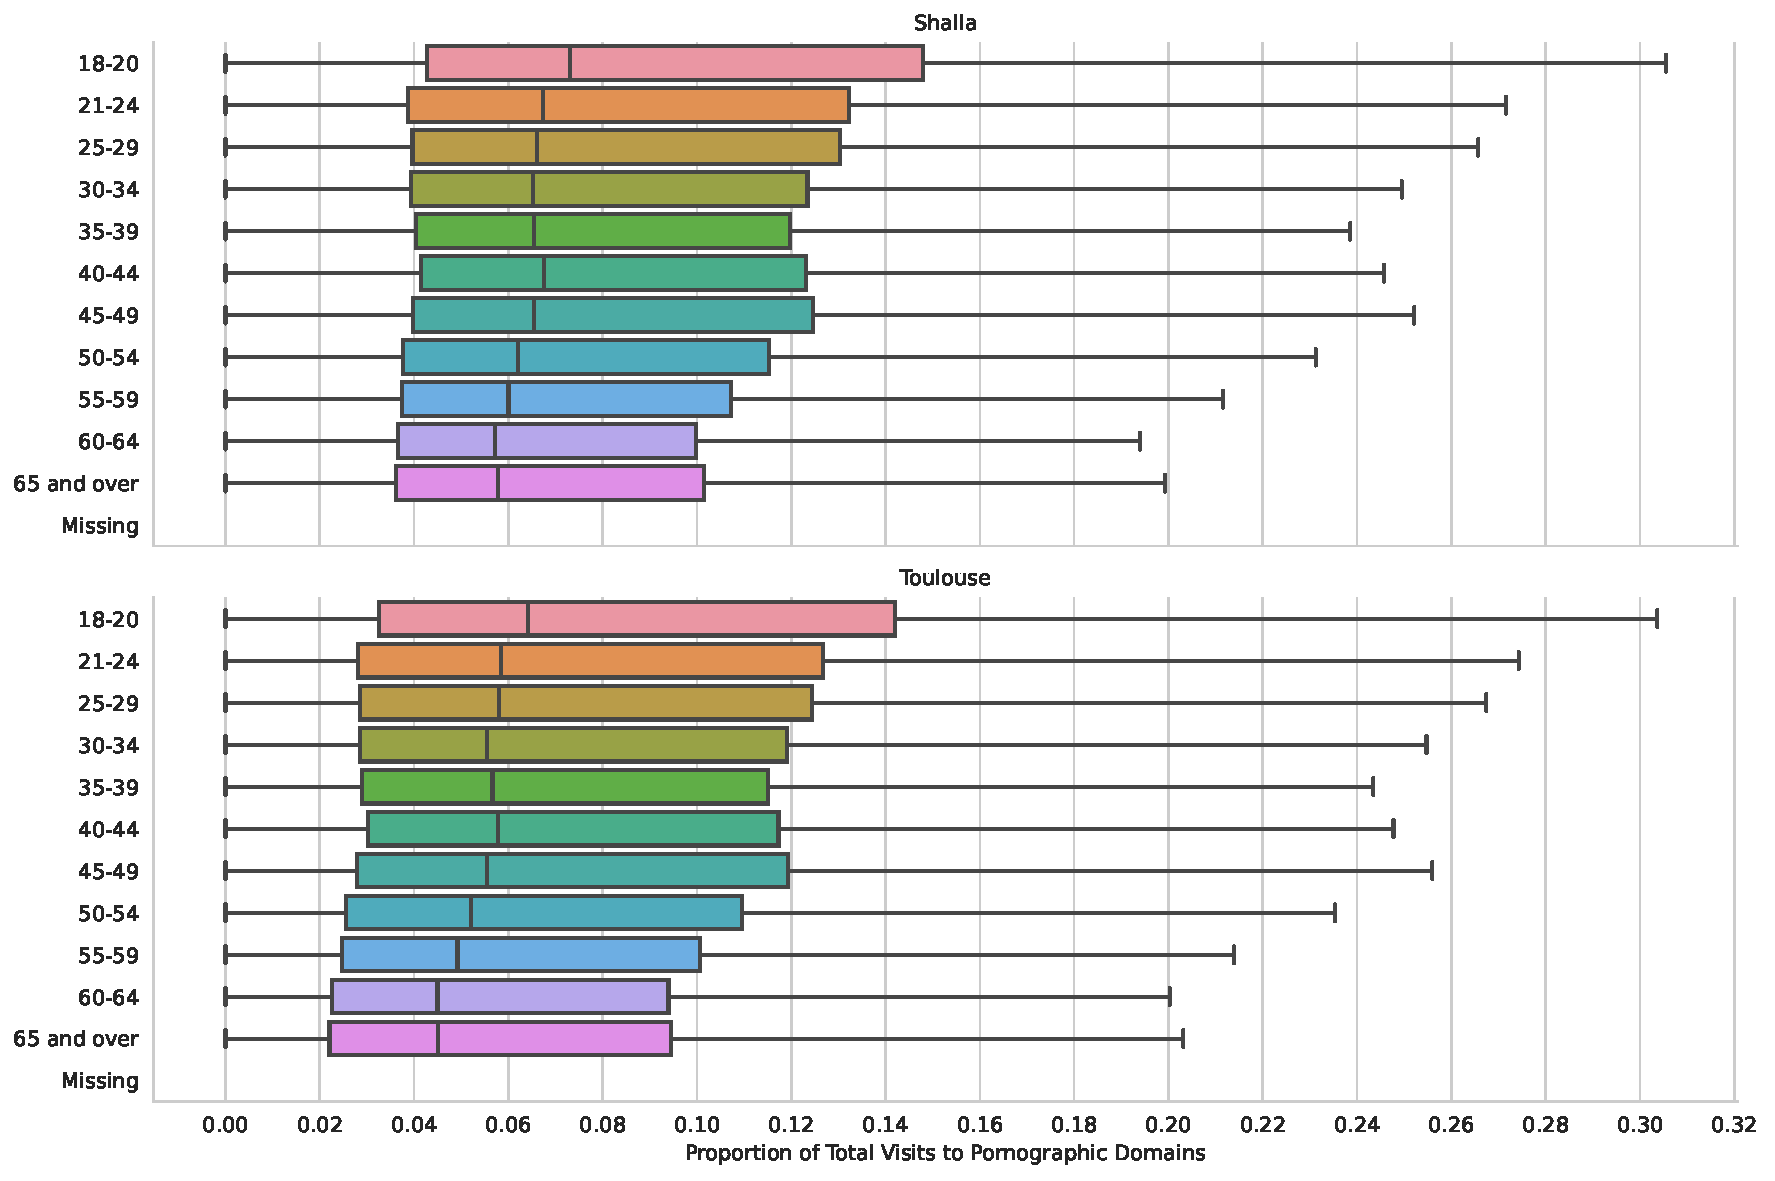
\includegraphics[width=\textwidth]{figs/prop_total_visits_porn_age.pdf}
\end{figure}

\section{Discussion}
You are what you browse. Which sites people visit reveals a lot about them and the challenges they face. The sites that people visit also affect their attitudes and behaviors. And in some cases, sites people visit also affect material outcomes. For instance, visiting a website that phishes personal information or hosts malware can lead to loss of personal information and money. Given the rich information that browsing data can give us, it is imperative to find accurate, light-weight, and scalable ways to learn what kind of content people are browsing.

In this paper, we contribute a solution to the problem. We present a new way to learn the kind of content hosted by the domain using the information in the domain name alone. We use LSTM to learn a model between the sequence of characters in a domain name and the kind of content it carries using multiple curated lists and the Alexa top 1M domains data. We find that we can learn good models for domains that host adult content with precision and recall around .9. Our models for classifying websites that carry harmful content do not work as well with f1-scores of about .8. We illustrate the utility of the models by using them to answer two interesting questions. We also provide a Python package that exposes the models: \url{https://github.com/themains/pydomains/}. The limitations of our models are that for gatekeeping tasks, the accuracy and recall may still be too low.
\clearpage
\bibliographystyle{apsr}
\bibliography{domain}
\clearpage
\appendix
\renewcommand{\thesection}{SI \arabic{section}}
\renewcommand\thetable{\thesection.\arabic{table}}
\renewcommand\thefigure{\thesection.\arabic{figure}}
\counterwithin{figure}{section}
\counterwithin{table}{section}

\section{Supporting Information}

\subsection{Data}

\begin{table}[h!]
\centering
\tiny
\caption{Number of unique domains by category in the Shallalist Dataset}
\begin{tabular}{ l c }
\hline
category               & n \\
\hline
adv                    & 12,712  \\
anonvpn                & 6,981   \\
downloads              & 4,177   \\
dynamic                & 1,066   \\
education/schools      & 10,068  \\
finance/banking        & 4,989   \\
finance/insurance      & 3,081   \\
finance/moneylending   & 3,802   \\
finance/realestate     & 1,379   \\
fortunetelling         & 1,077   \\
forum                  & 8,058   \\
gamble                 & 13,827  \\
hobby/games-online     & 13,861  \\
hobby/pets             & 16,164  \\
hospitals              & 1,637   \\
jobsearch              & 4,294   \\
movies                 & 5,558   \\
music                  & 8,918   \\
others                 & 110,991 \\
porn                   & 827,444 \\
radiotv                & 3,560   \\
recreation/restaurants & 1,408   \\
recreation/sports      & 120,426 \\
recreation/travel      & 138,943 \\
redirector             & 29,366  \\
religion               & 9,189   \\
science/astronomy      & 1,035   \\
sex/lingerie           & 1,056   \\
shopping               & 167,262 \\
webmail                & 3,525   \\
webradio               & 2,254  \\
\hline
\end{tabular}
\label{tab:shalla_data}
\end{table}

\begin{table}[h!]
\centering
\tiny
\caption{Number of unique domains by category in the Toulouse Dataset}
\begin{tabular}{ l c }
\hline
category  & n \\
\hline
adult     & 187,0741 \\
bank      & 1,689 \\
gambling  &  1,012 \\
games     &  9,357 \\
malware   &  4,463 \\
others    &  21,441 \\
phishing  &  62,712 \\
press     &  4,410 \\
shopping  &  36,331 \\
\hline
\end{tabular}
\label{tab:toulouse_data}
\end{table}
\clearpage

\subsection{Model Performance}

\begin{table}[!htb]
\centering
\tiny
\caption{OOS Performance of the Malware LSTM Model}
\begin{tabular}{ l c c c c }
\hline
    malware or not & precision & recall & f1-score & support \\
\hline
      0  &         0.86 &     0.95   &    0.91  &   10,000\\
      1  &         0.77 &     0.51   &    0.61  &   3,048 \\
weighted avg  &     0.84 &     0.85   &    0.84  &   13,048 \\
\hline
\end{tabular}
\label{tab:malware_model}
\end{table}

\begin{table}[!htb]
\centering
\tiny
\caption{OOS Performance of the PhishTank LSTM Model}
\begin{tabular}{ l c c c c }
\hline
    phishing or not & precision & recall & f1-score & support \\
\hline
      0  &         0.79 &     0.90   &    0.84  &   10,000\\
      1  &         0.89 &     0.76   &    0.82  &   10,000 \\
weighted avg  &     0.84 &     0.83   &    0.83  &   20,000 \\
\hline
\end{tabular}
\label{tab:phishtank_model}
\end{table}

\begin{table}[!htb]
\centering
\tiny
\caption{OOS Performance of the Shalla LSTM Model}
\begin{tabular}{ l c c c c }
\hline
categories      & precision & recall & f1-score & support \\
\hline
                   adv   &     0.80  &    0.41  &    0.54   &   2,542 \\
               anonvpn   &     0.80  &    0.68  &    0.74   &   1,396 \\
             downloads   &     0.54  &    0.38  &    0.45   &    835 \\
               dynamic   &     0.81  &    0.54  &    0.65   &    213 \\
     education/schools   &     0.89  &    0.78  &    0.83   &   2,014 \\
       finance/banking   &     0.79  &    0.53  &    0.64   &    998 \\
     finance/insurance   &     0.96  &    0.82  &    0.88   &    616 \\
  finance/moneylending   &     0.86  &    0.80  &    0.83   &    760 \\
    finance/realestate   &     0.69  &    0.39  &    0.50   &    276 \\
        fortunetelling   &     0.71  &    0.35  &    0.47   &    215 \\
                 forum   &     0.73  &    0.80  &    0.77   &   1,612 \\
                gamble   &     0.83  &    0.75  &    0.79   &   2,765 \\
    hobby/games-online   &     0.68  &    0.48  &    0.56   &   2,772 \\
            hobby/pets   &     0.66  &    0.34  &    0.45   &   3,233 \\
             hospitals   &     0.83  &    0.69  &    0.75   &    327 \\
             jobsearch   &     0.83  &    0.46  &    0.59   &    859 \\
                movies   &     0.68  &    0.47  &    0.56   &   1,112 \\
                 music   &     0.85  &    0.85  &    0.85   &   1,784 \\
                others   &     0.49  &    0.30  &    0.37   &  22,198 \\
                  porn   &     0.85  &    0.93  &    0.89   & 165,489 \\
               radiotv   &     0.61  &    0.48  &    0.54   &    712 \\
recreation/restaurants   &     0.79  &    0.28  &    0.41   &    282 \\
     recreation/sports   &     0.64  &    0.63  &    0.64   &  24,085 \\
     recreation/travel   &     0.71  &    0.65  &    0.68   &  27,789 \\
            redirector   &     0.84  &    0.66  &    0.74   &   5,873 \\
              religion   &     0.90  &    0.82  &    0.86   &   1,838 \\
     science/astronomy   &     0.69  &    0.87  &    0.77   &    207 \\
          sex/lingerie   &     0.41  &    0.45  &    0.42   &    211 \\
              shopping   &     0.54  &    0.62  &    0.58   &  33,453 \\
               webmail   &     0.78  &    0.56  &    0.65   &    705 \\
              webradio   &     0.48  &    0.47  &    0.48   &    451 \\
          weighted avg   &     0.76  &    0.76  &    0.76   &  307,622 \\
\hline
\end{tabular}
\label{tab:shalla_model}
\end{table}

\begin{table}[!htb]
\centering
\tiny
\caption{OOS Performance of the Toulouse/Squidguard LSTM Model}
\begin{tabular}{ l c c c c }
\hline
categories  & precision & recall & f1-score & support \\
\hline
	   adult     & 0.97    & 0.99    & 0.98    & 374,149 \\
        bank     & 0.68    & 0.56    & 0.61    & 338 \\
    gambling     & 0.49    & 0.18    & 0.27    & 202 \\
       games     & 0.84    & 0.45    & 0.58    & 1,871 \\
     malware     & 0.97    & 0.48    & 0.64    & 893 \\
      others     & 0.60    & 0.19    & 0.28    & 4,288 \\
    phishing     & 0.72    & 0.60    & 0.65    & 12,543 \\
       press     & 0.78    & 0.53    & 0.63    & 882 \\
    shopping     & 0.67    & 0.44    & 0.53    & 7,266 \\
weighted avg     & 0.95    & 0.96    & 0.95    & 402,432 \\
\hline
\end{tabular}
\label{tab:toulouse_model}
\end{table}

\clearpage
\subsection{Supplementary Results}

\begin{figure}[!htb]
  \centering
  \caption{Time Spent on Phishing/Malware Domains by Education}
	\label{fig:total_time_phishing_malware_educ}
	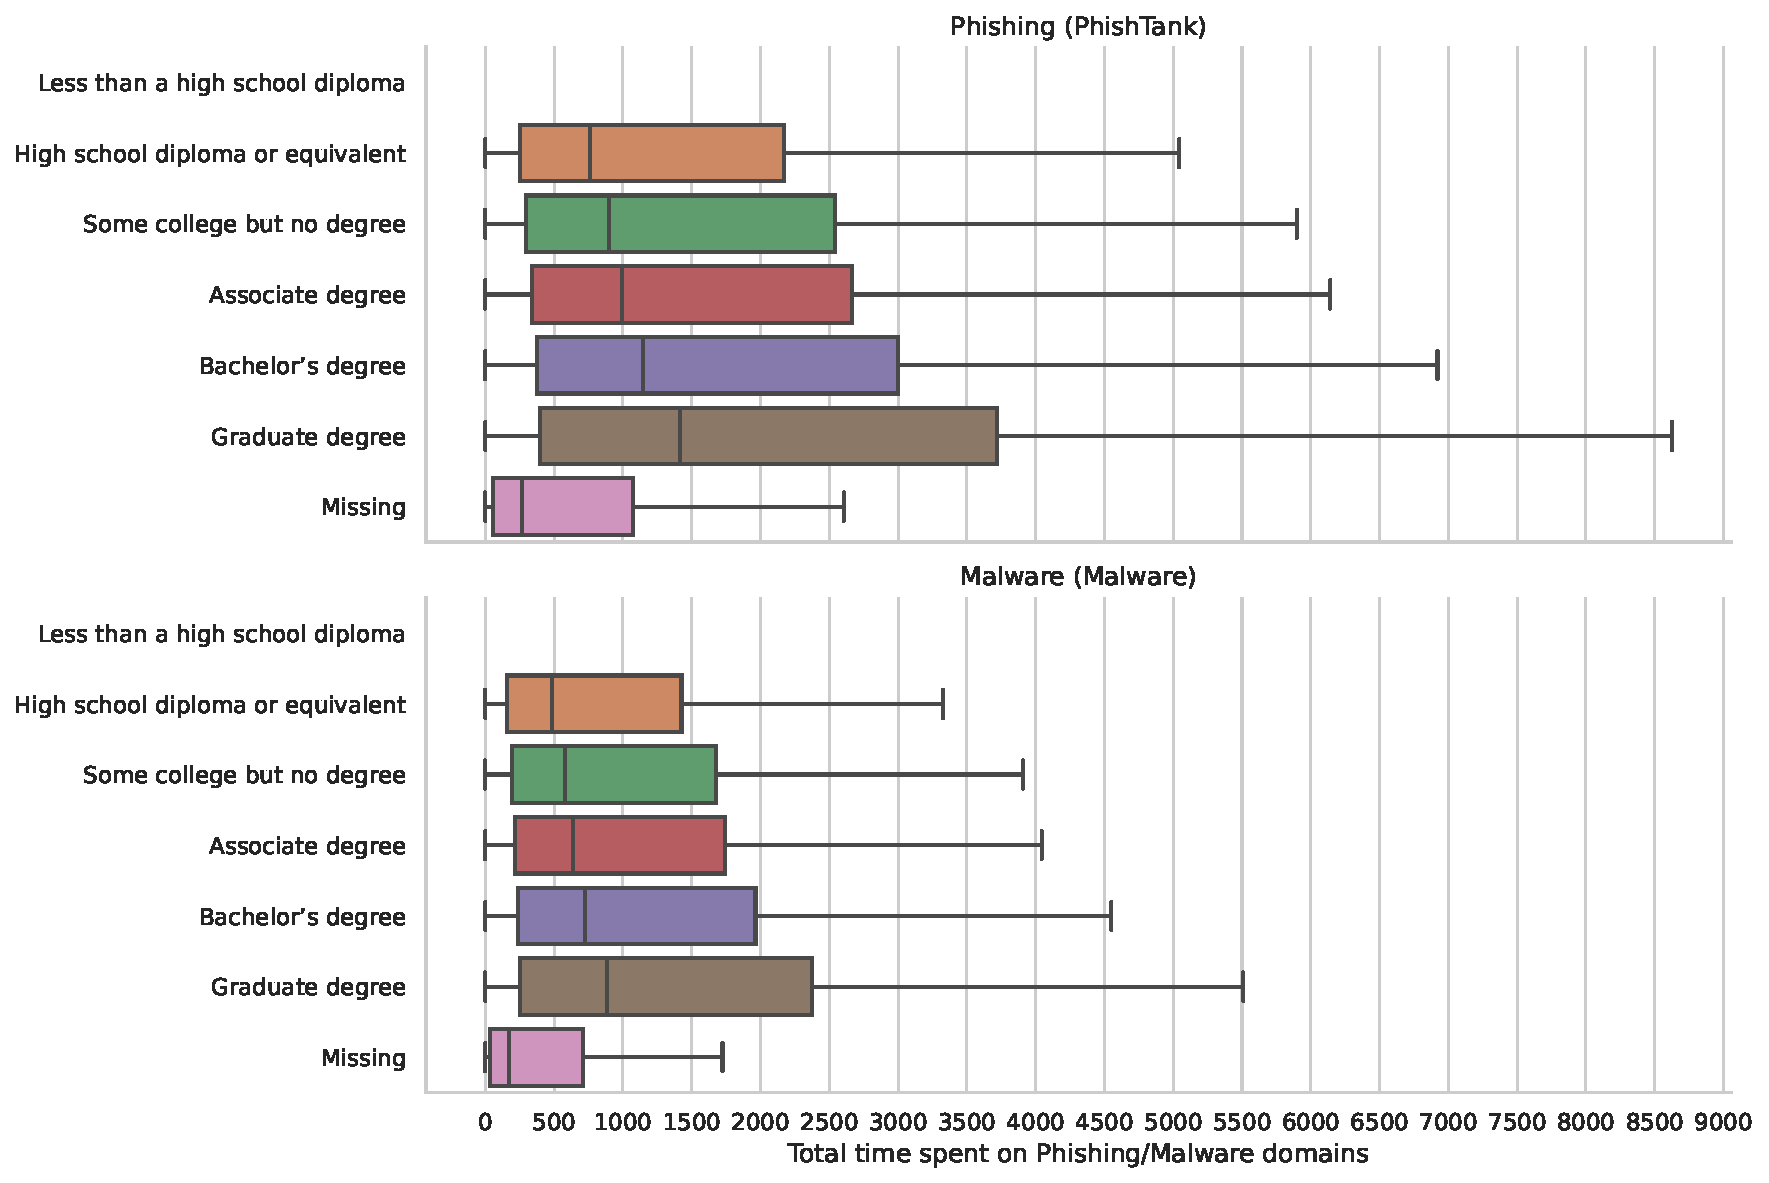
\includegraphics[width=\textwidth]{figs/total_time_phishing_malware_educ.pdf}
\end{figure}

\begin{figure}[!htb]
  \centering
  \caption{Time Spent on Phishing/Malware Domains by Race}
	\label{fig:prop_total_time_phishing_malware_race}
	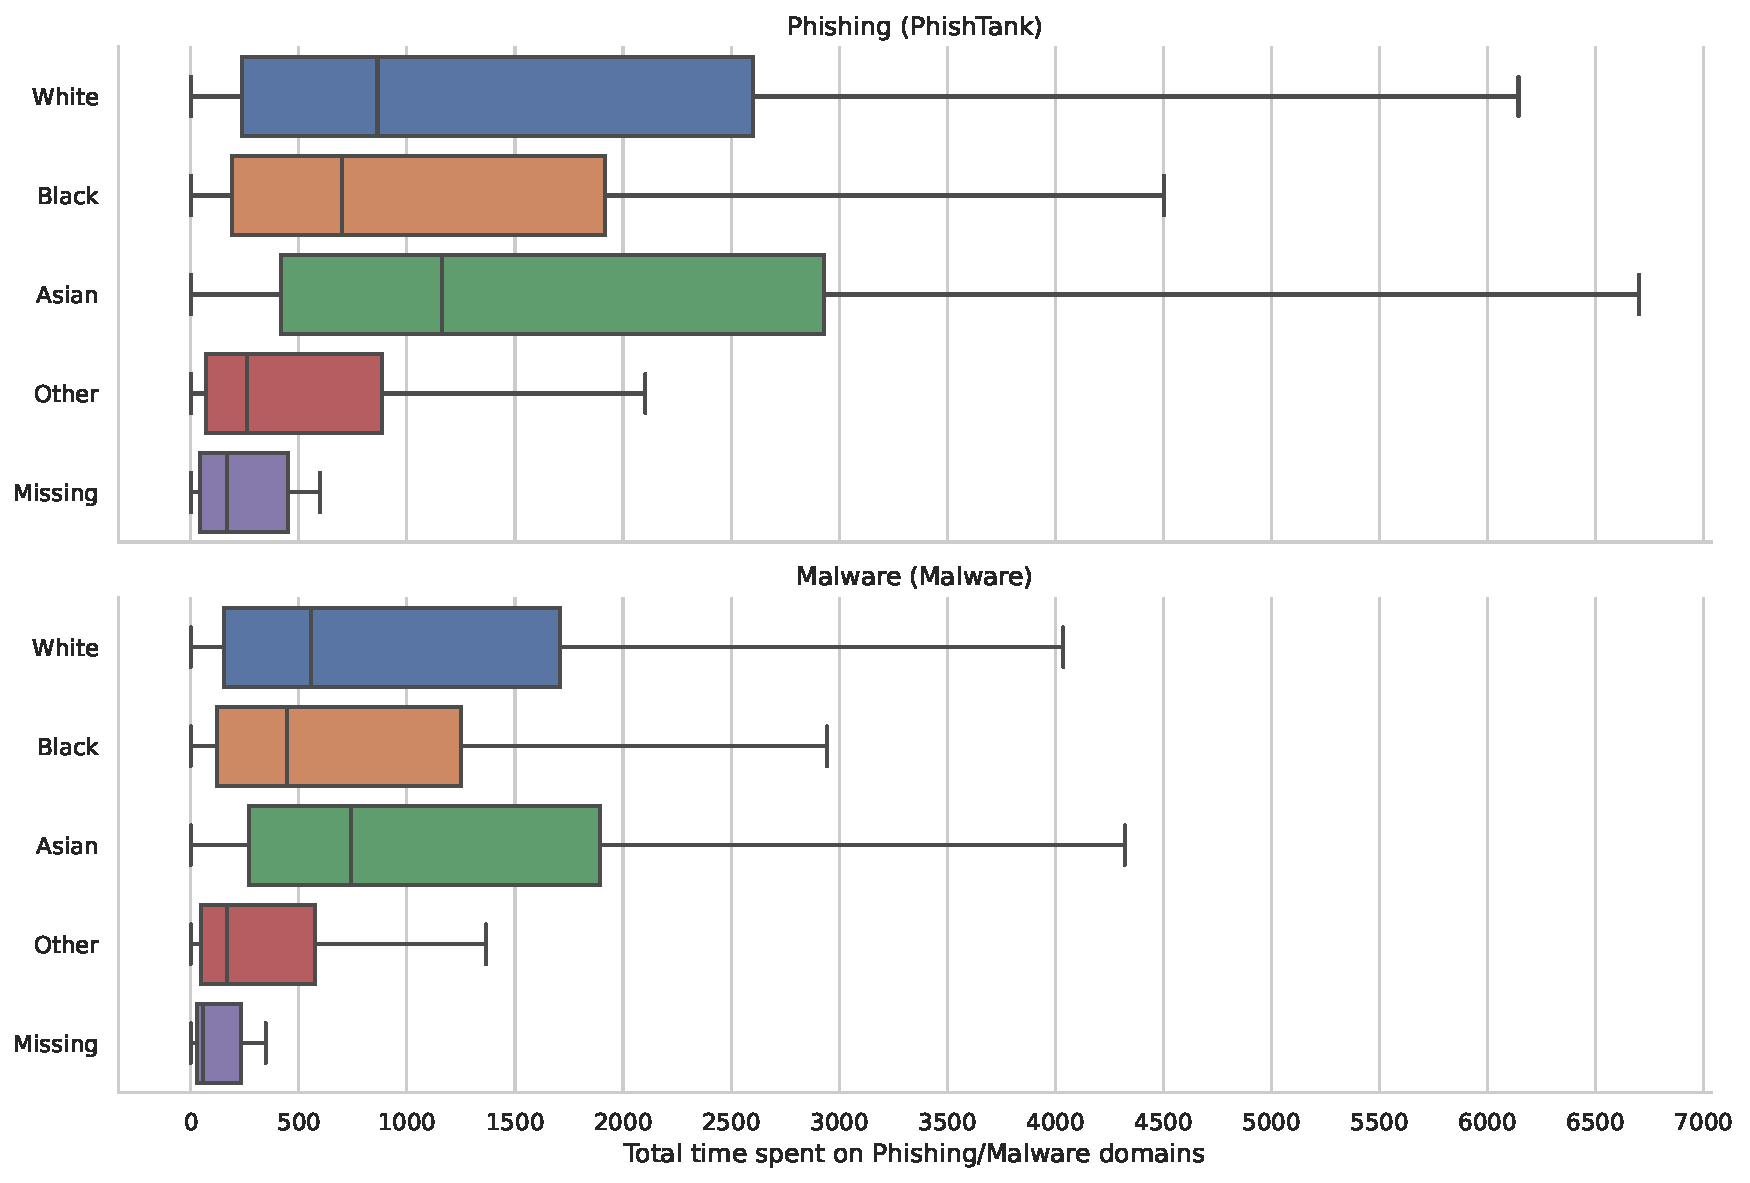
\includegraphics[width=\textwidth]{figs/total_time_phishing_malware_race.pdf}
	\end{figure}

\begin{figure}[!htb]
	 \centering
	 \caption{Time Spent on Phishing/Malware Domains by Age}
	 \label{fig:prop_total_time_phishing_malware_age}
	 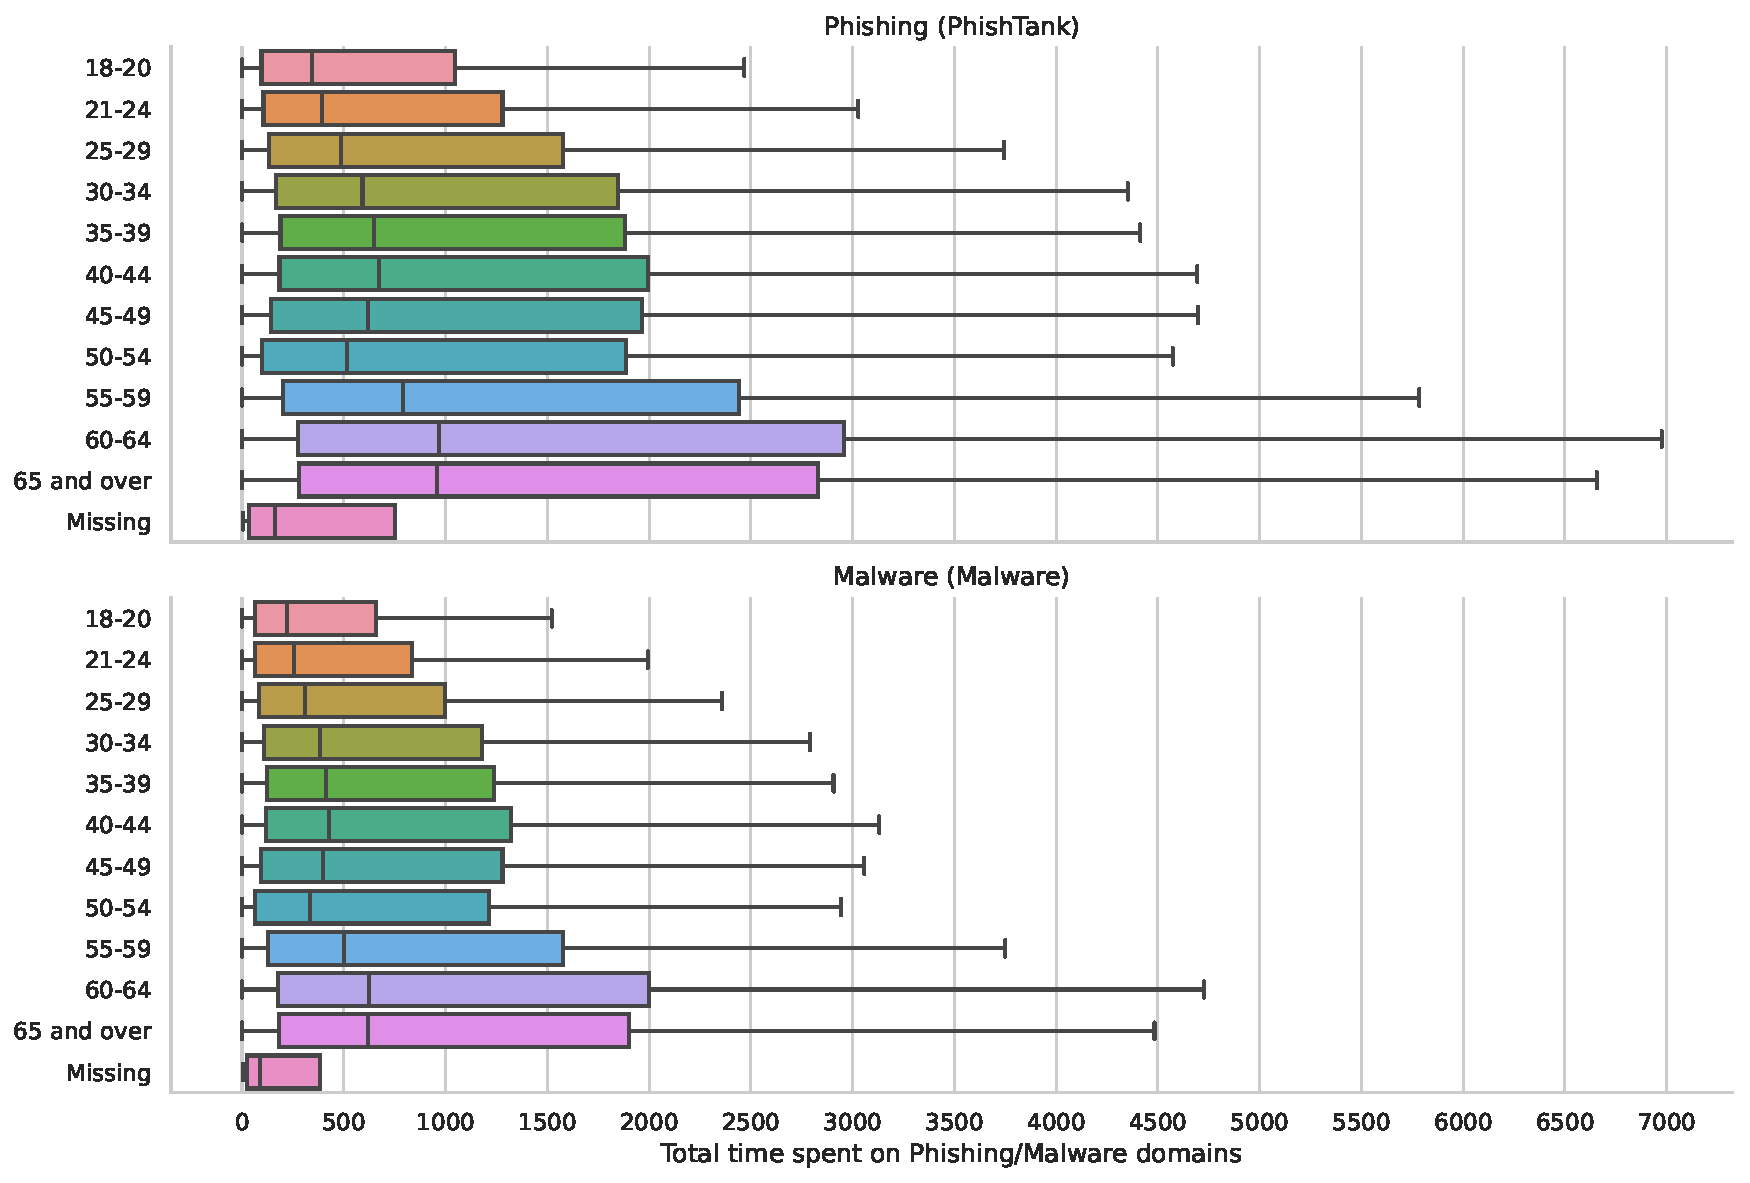
\includegraphics[width=\textwidth]{figs/total_time_phishing_malware_age.pdf}
\end{figure}

\begin{figure}[!htb]
\centering
\caption{Proportion of Time Spent on Phishing/Malware Domains by Education}
	\label{fig:prop_total_time_phishing_malware_educ}
	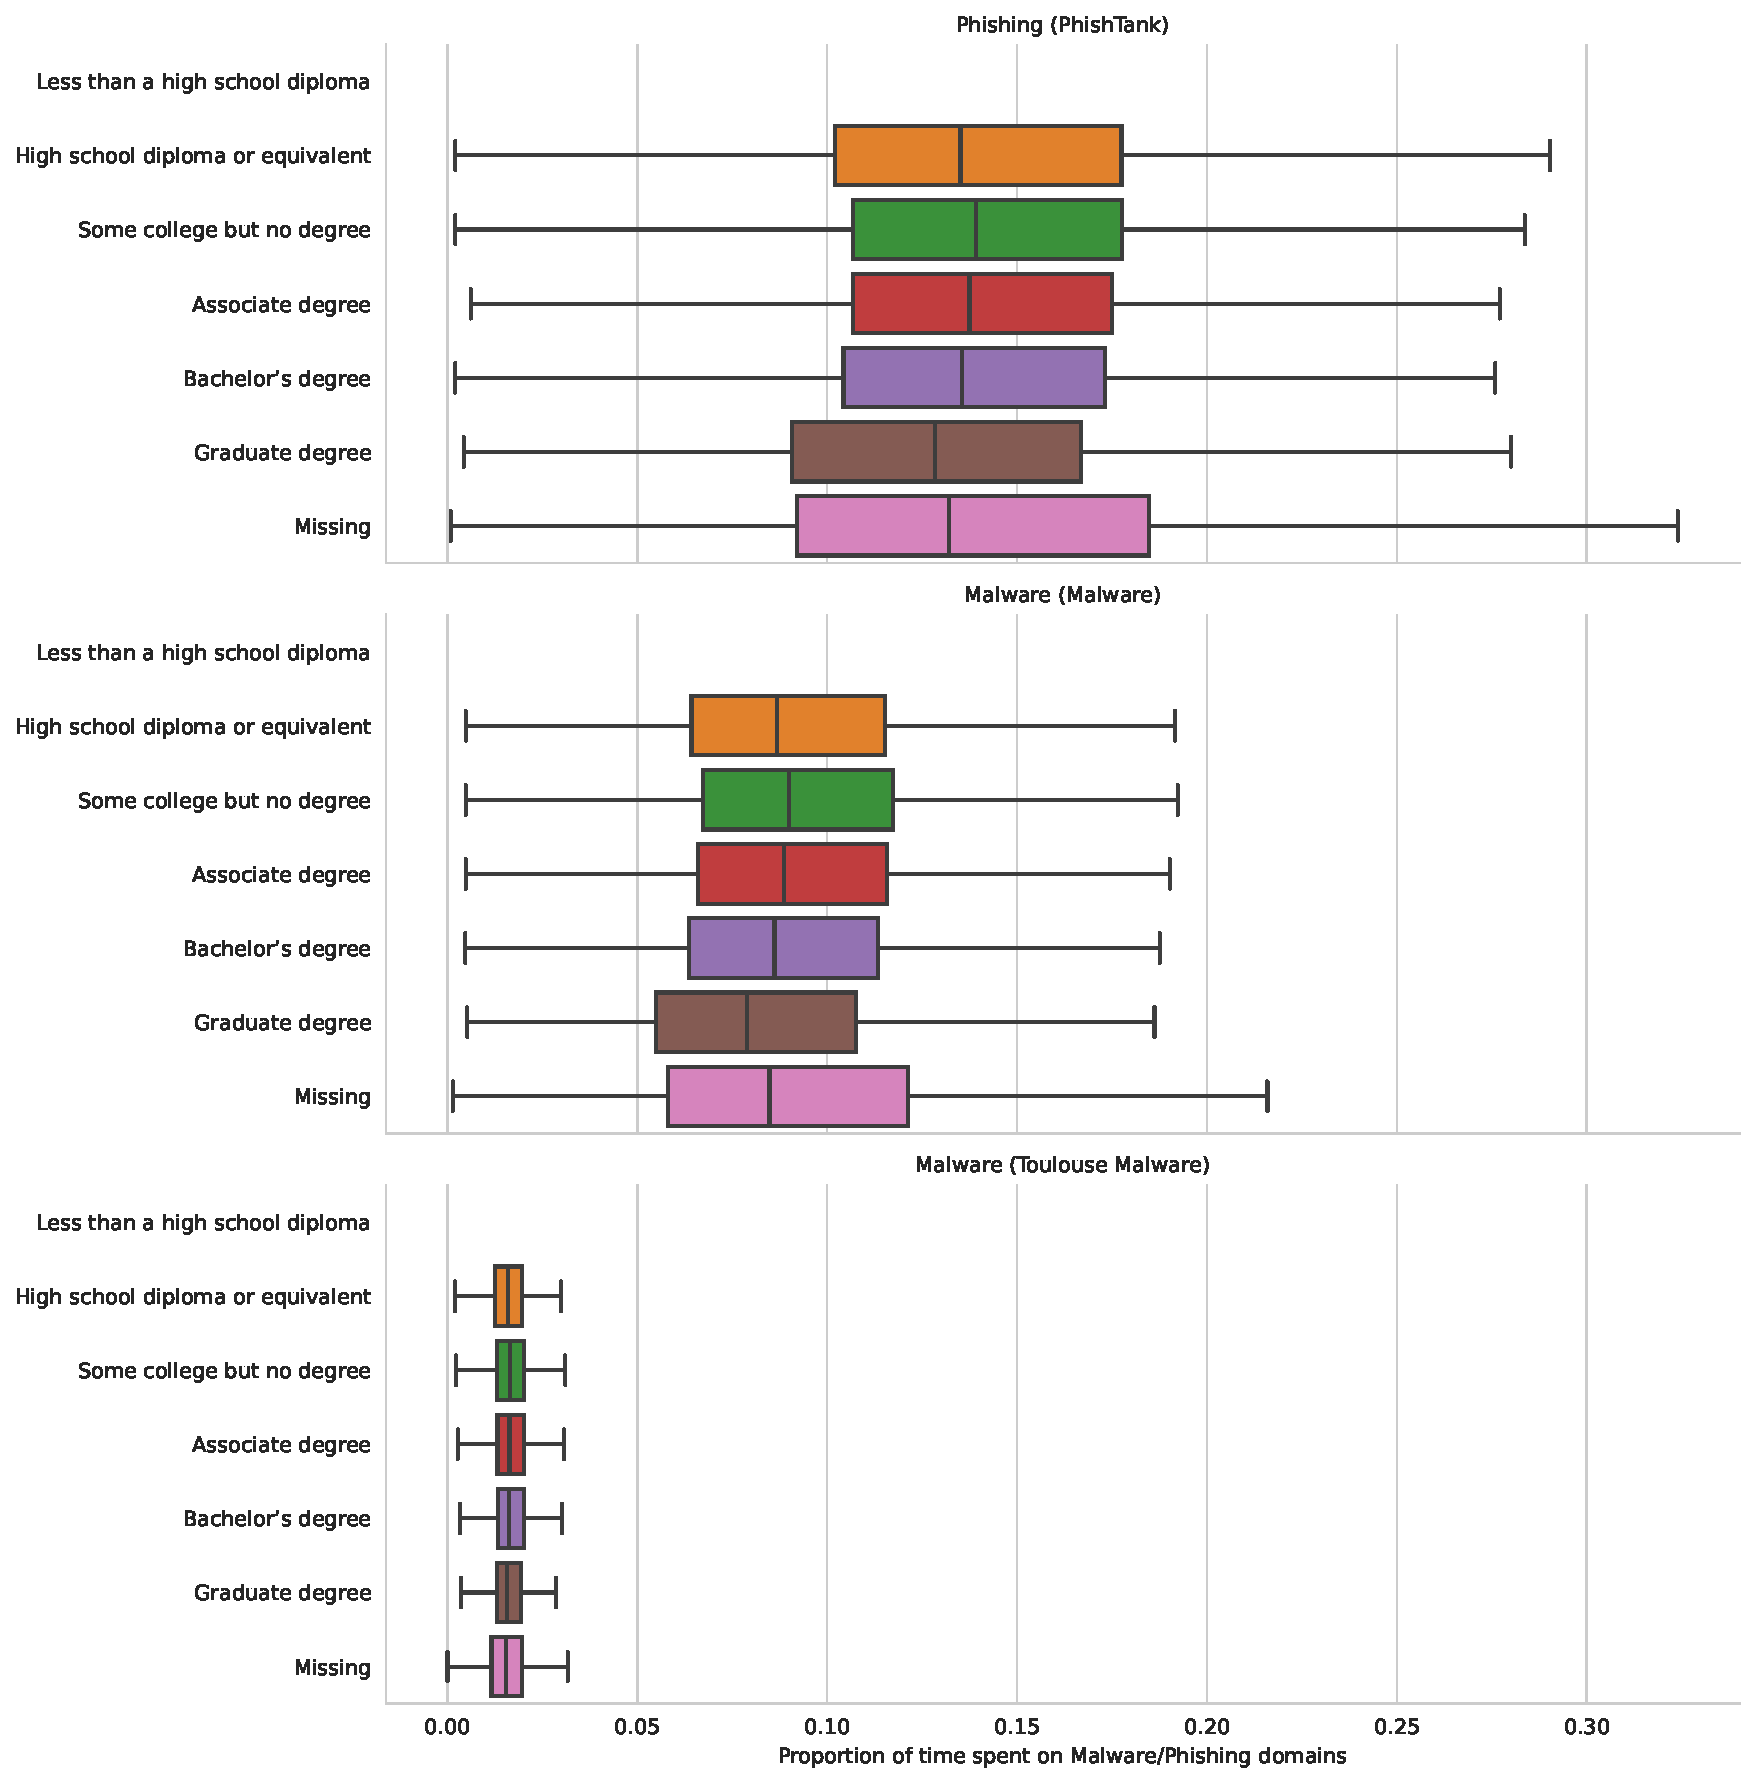
\includegraphics[width=\textwidth]{figs/prop_total_time_phishing_malware_tl_educ.pdf}
\end{figure}

\begin{figure}[!htb]
	 \centering
	 \caption{Proportion of Time Spent on Phishing/Malware Domains by Race}
	 \label{fig:prop_total_time_phishing_malware_race}
	 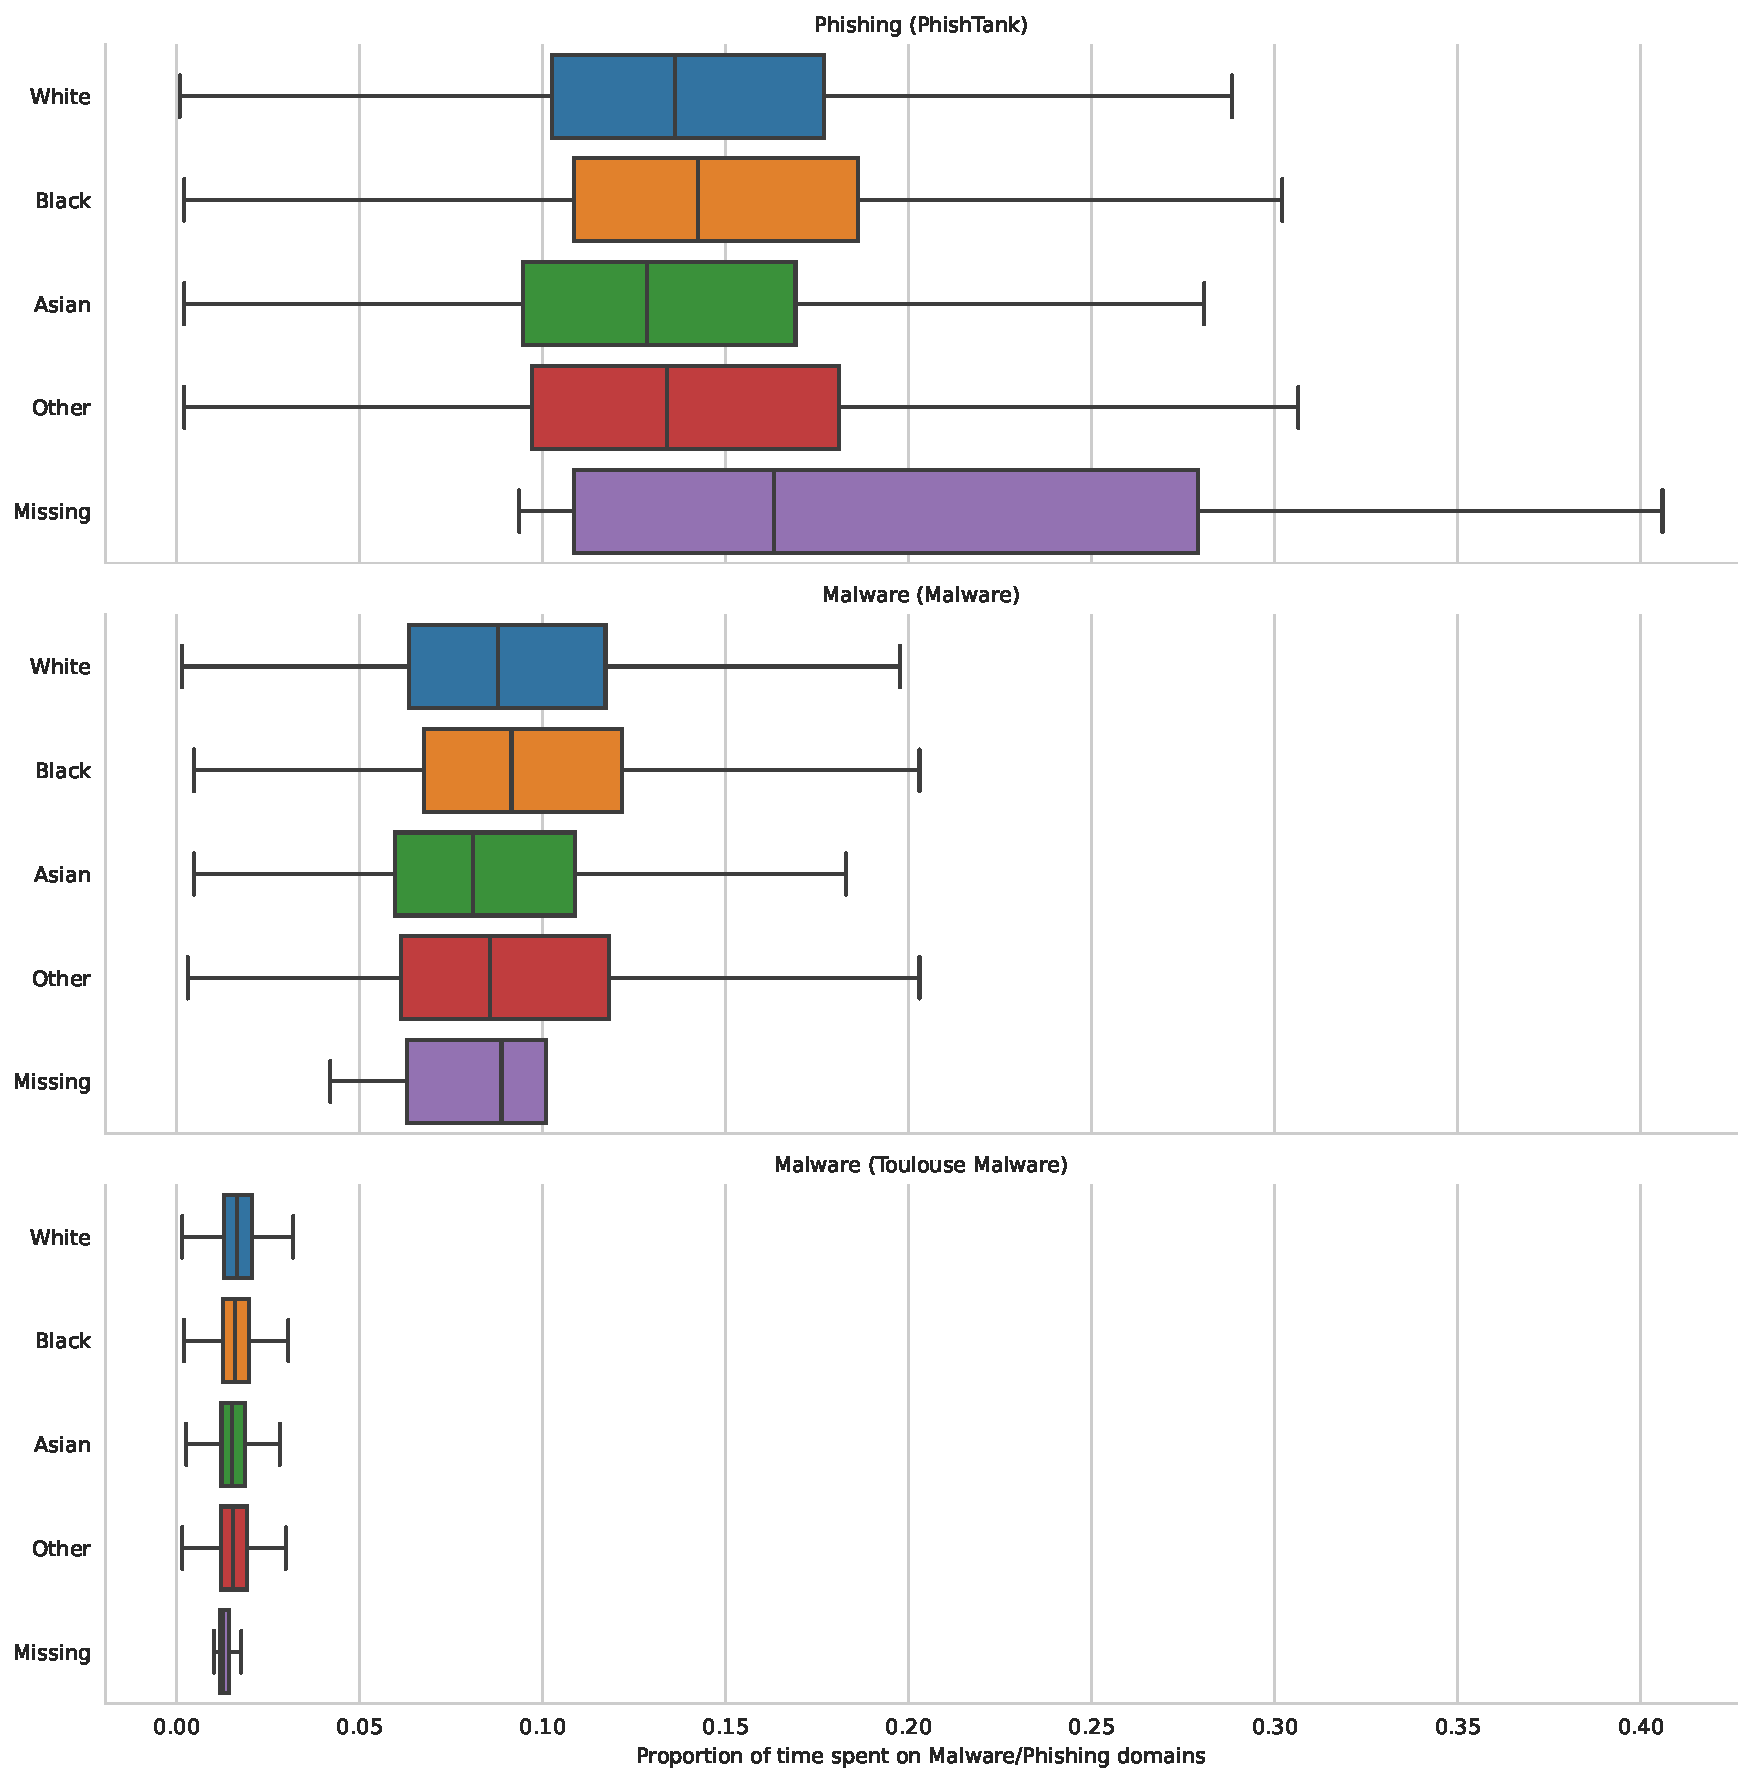
\includegraphics[width=\textwidth]{figs/prop_total_time_phishing_malware_tl_race.pdf}
\end{figure}

\begin{figure}[!htb]
	 \centering
	 \caption{Proportion of Time Spent on Phishing/Malware Domains by Age}
	 \label{prop_total_time_phishing_malware_age}
	 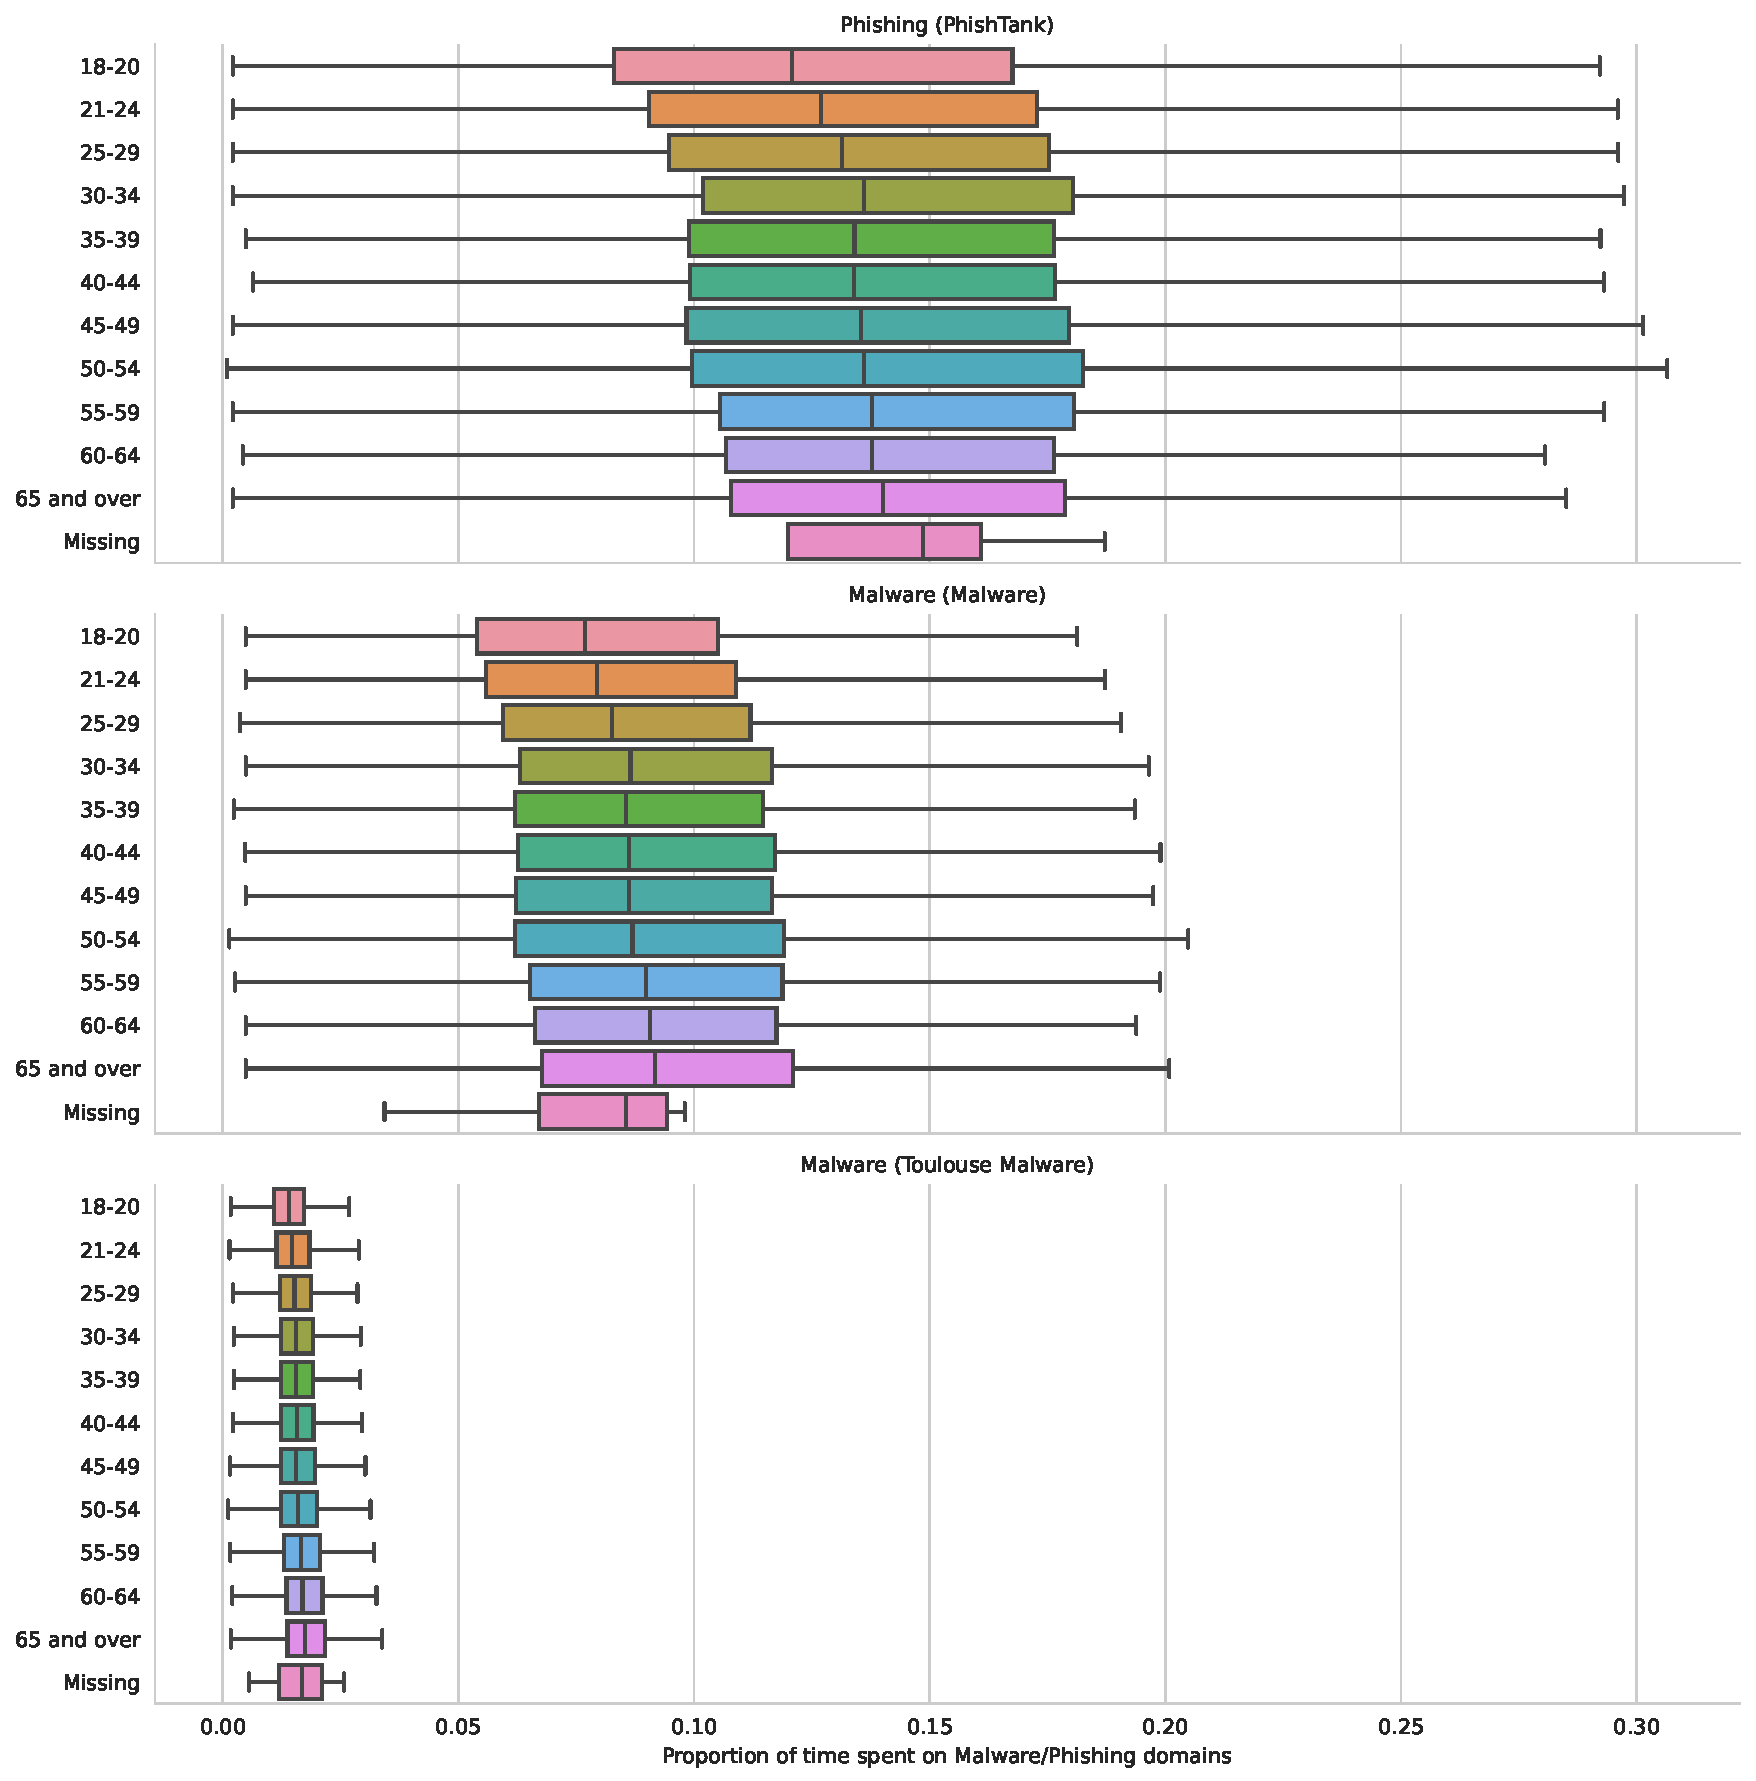
\includegraphics[width=\textwidth]{figs/prop_total_time_phishing_malware_tl_age.pdf}
\end{figure}

\begin{figure}[!htb]
  \centering
  \caption{Proportion of Visits to Phishing/Malware Domains by Education}
	\label{fig:prop_total_visits_phishing_malware_educ}
	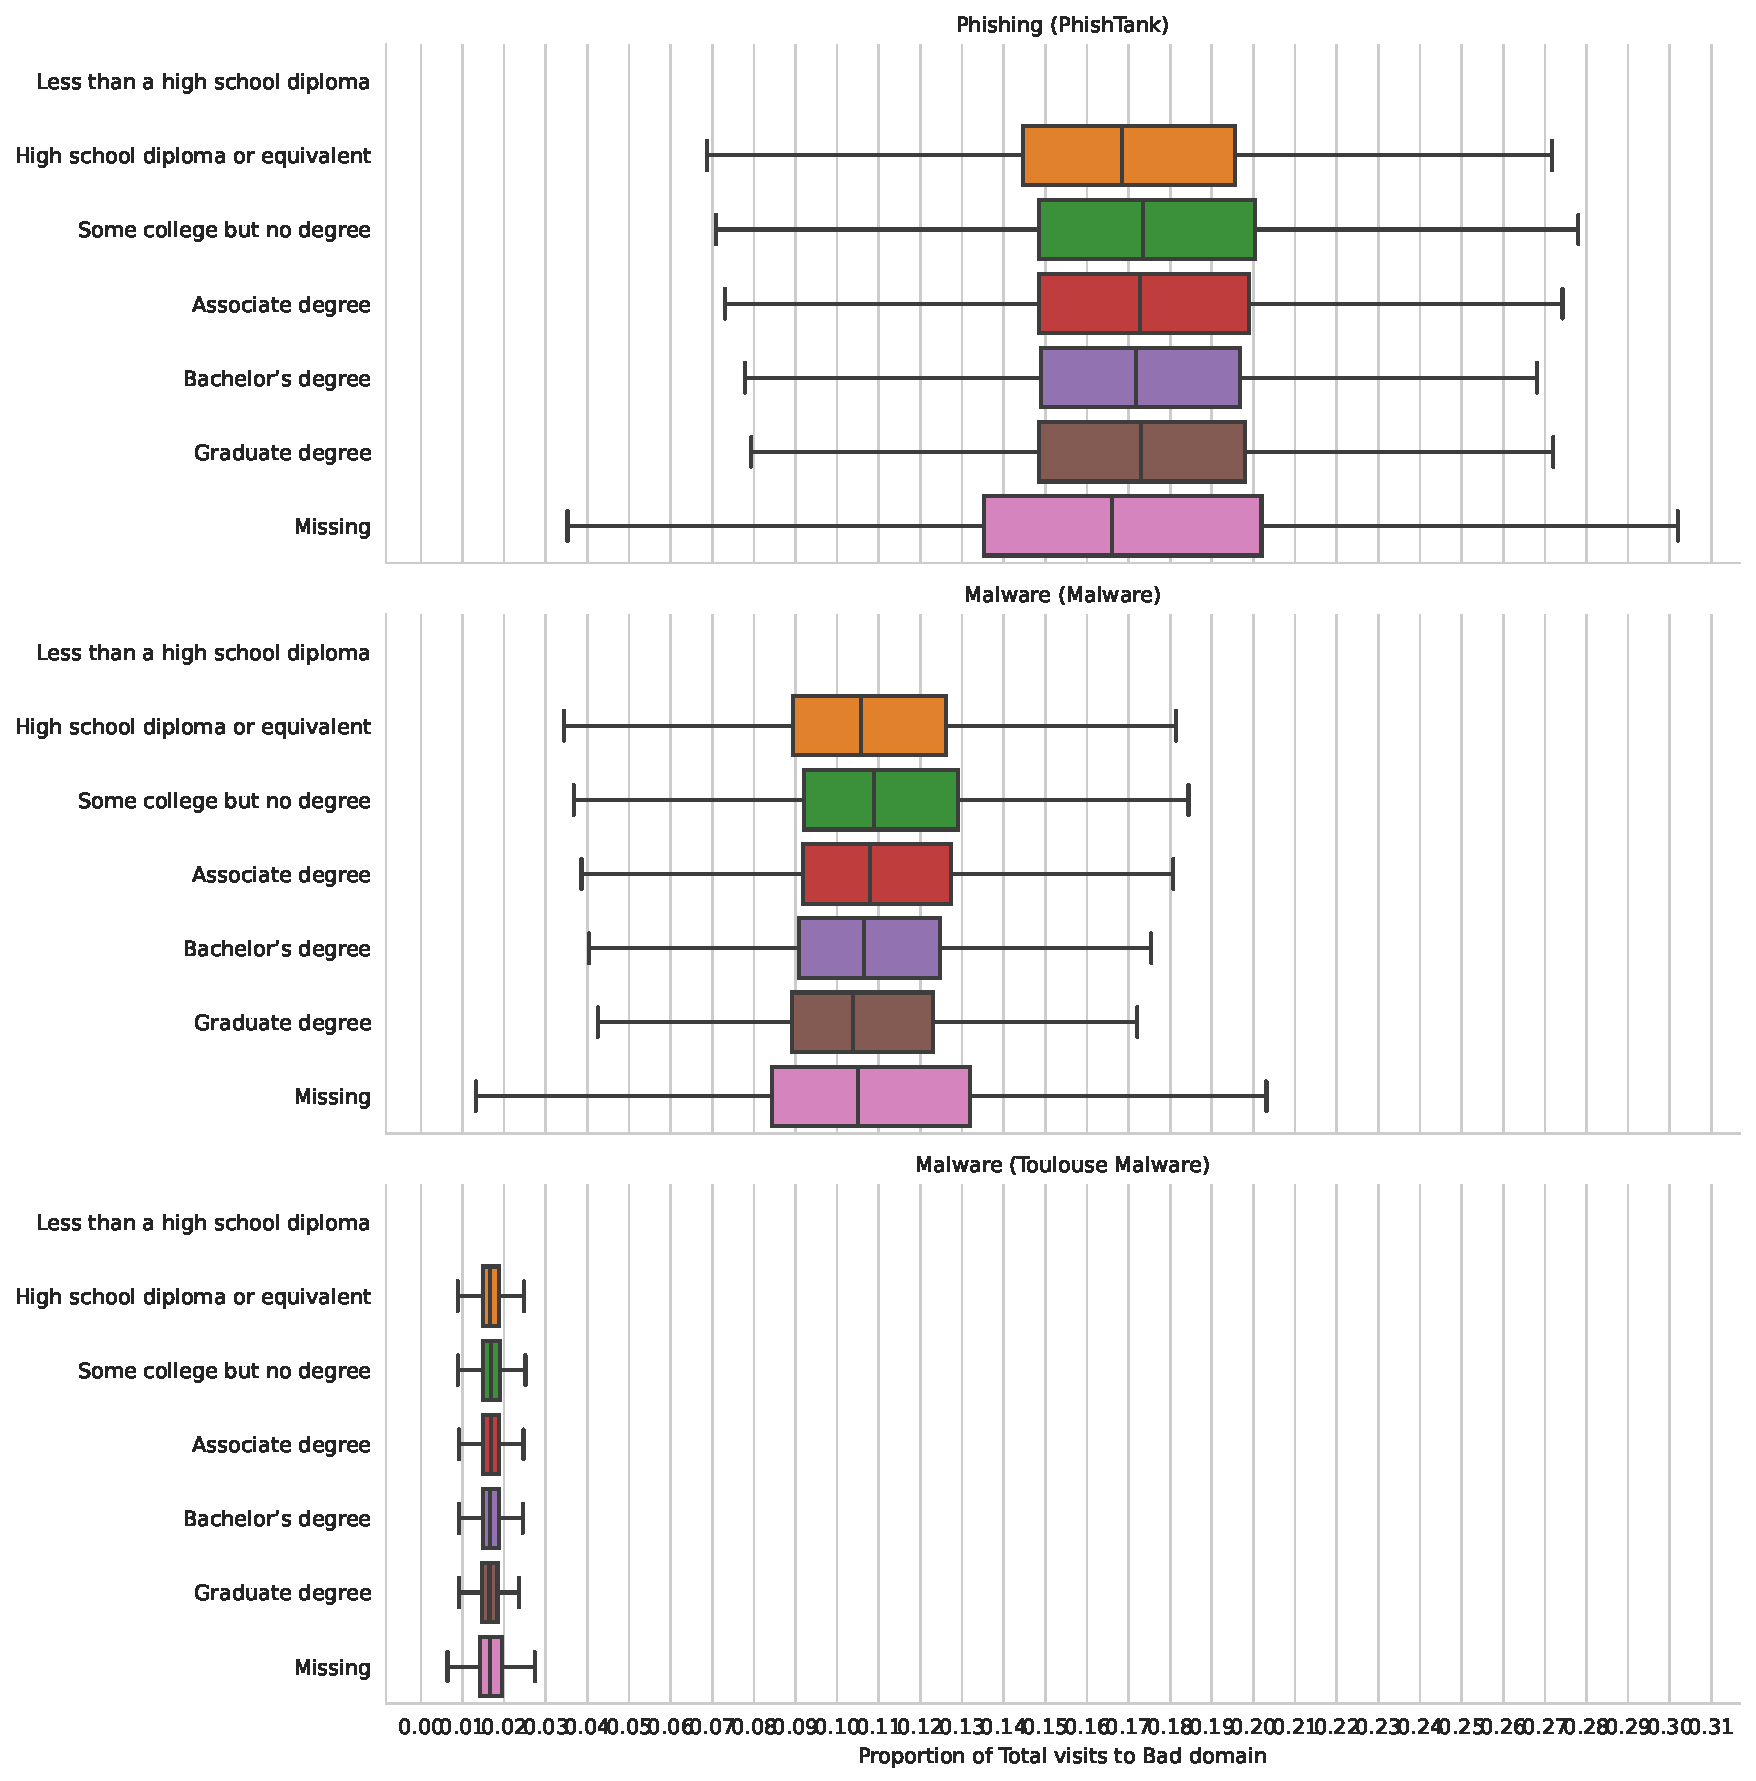
\includegraphics[width=\textwidth]{figs/prop_total_visits_phishing_malware_tl_educ.pdf}
\end{figure}

\begin{figure}[!htb]
  \centering
  \caption{Time Spent on Pornographic Domains by Education}
  \label{fig:total_time_porn_educ}
  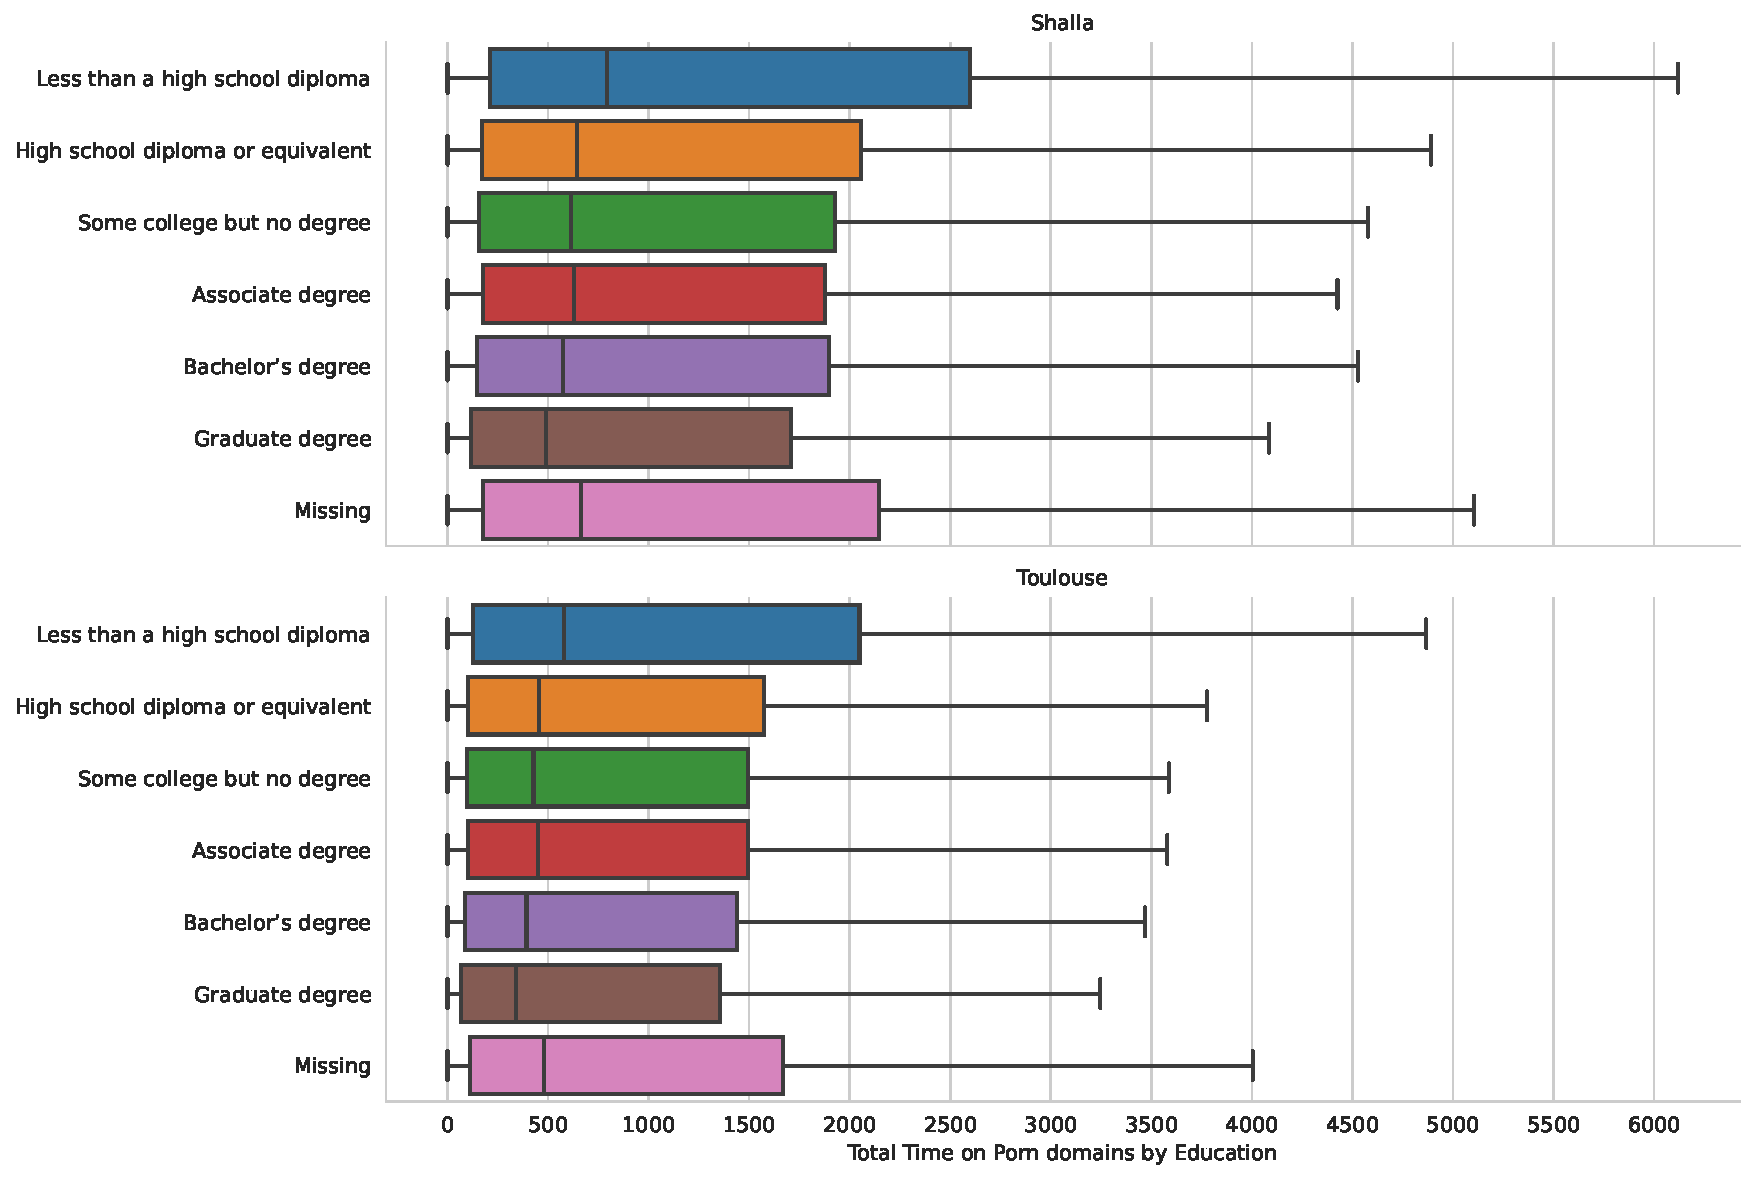
\includegraphics[width=\textwidth]{figs/total_time_porn_educ.pdf}
\end{figure}

\begin{figure}[!htb]
  \centering
  \caption{Time Spent on Pornographic Domains by Age}
  \label{fig:total_time_porn_age}
  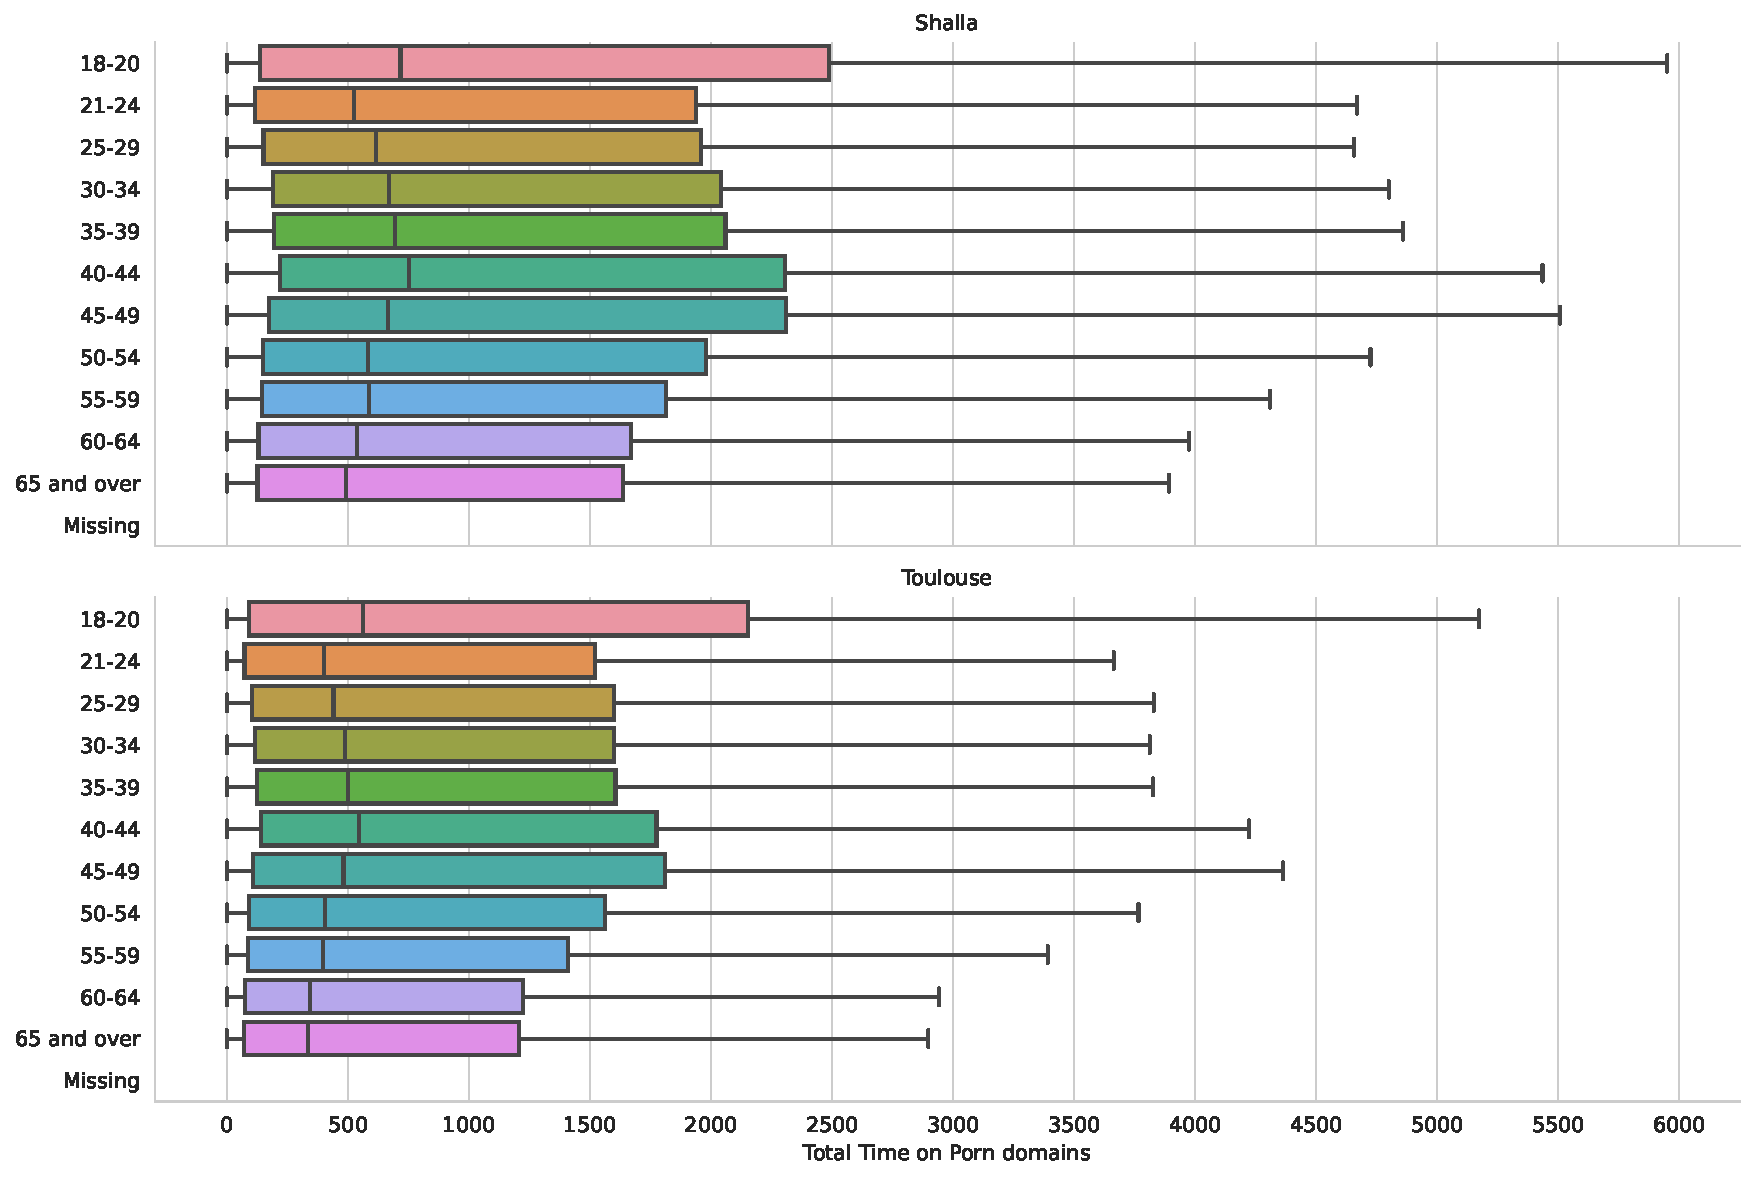
\includegraphics[width=\textwidth]{figs/total_time_porn_age.pdf}\\Age
\end{figure}

\begin{figure}[!htb]
  \centering
  \caption{Proportion of Visits to Phishing/Malware Domains by Race}
	\label{fig:prop_total_visits_phishing_malware_race}
	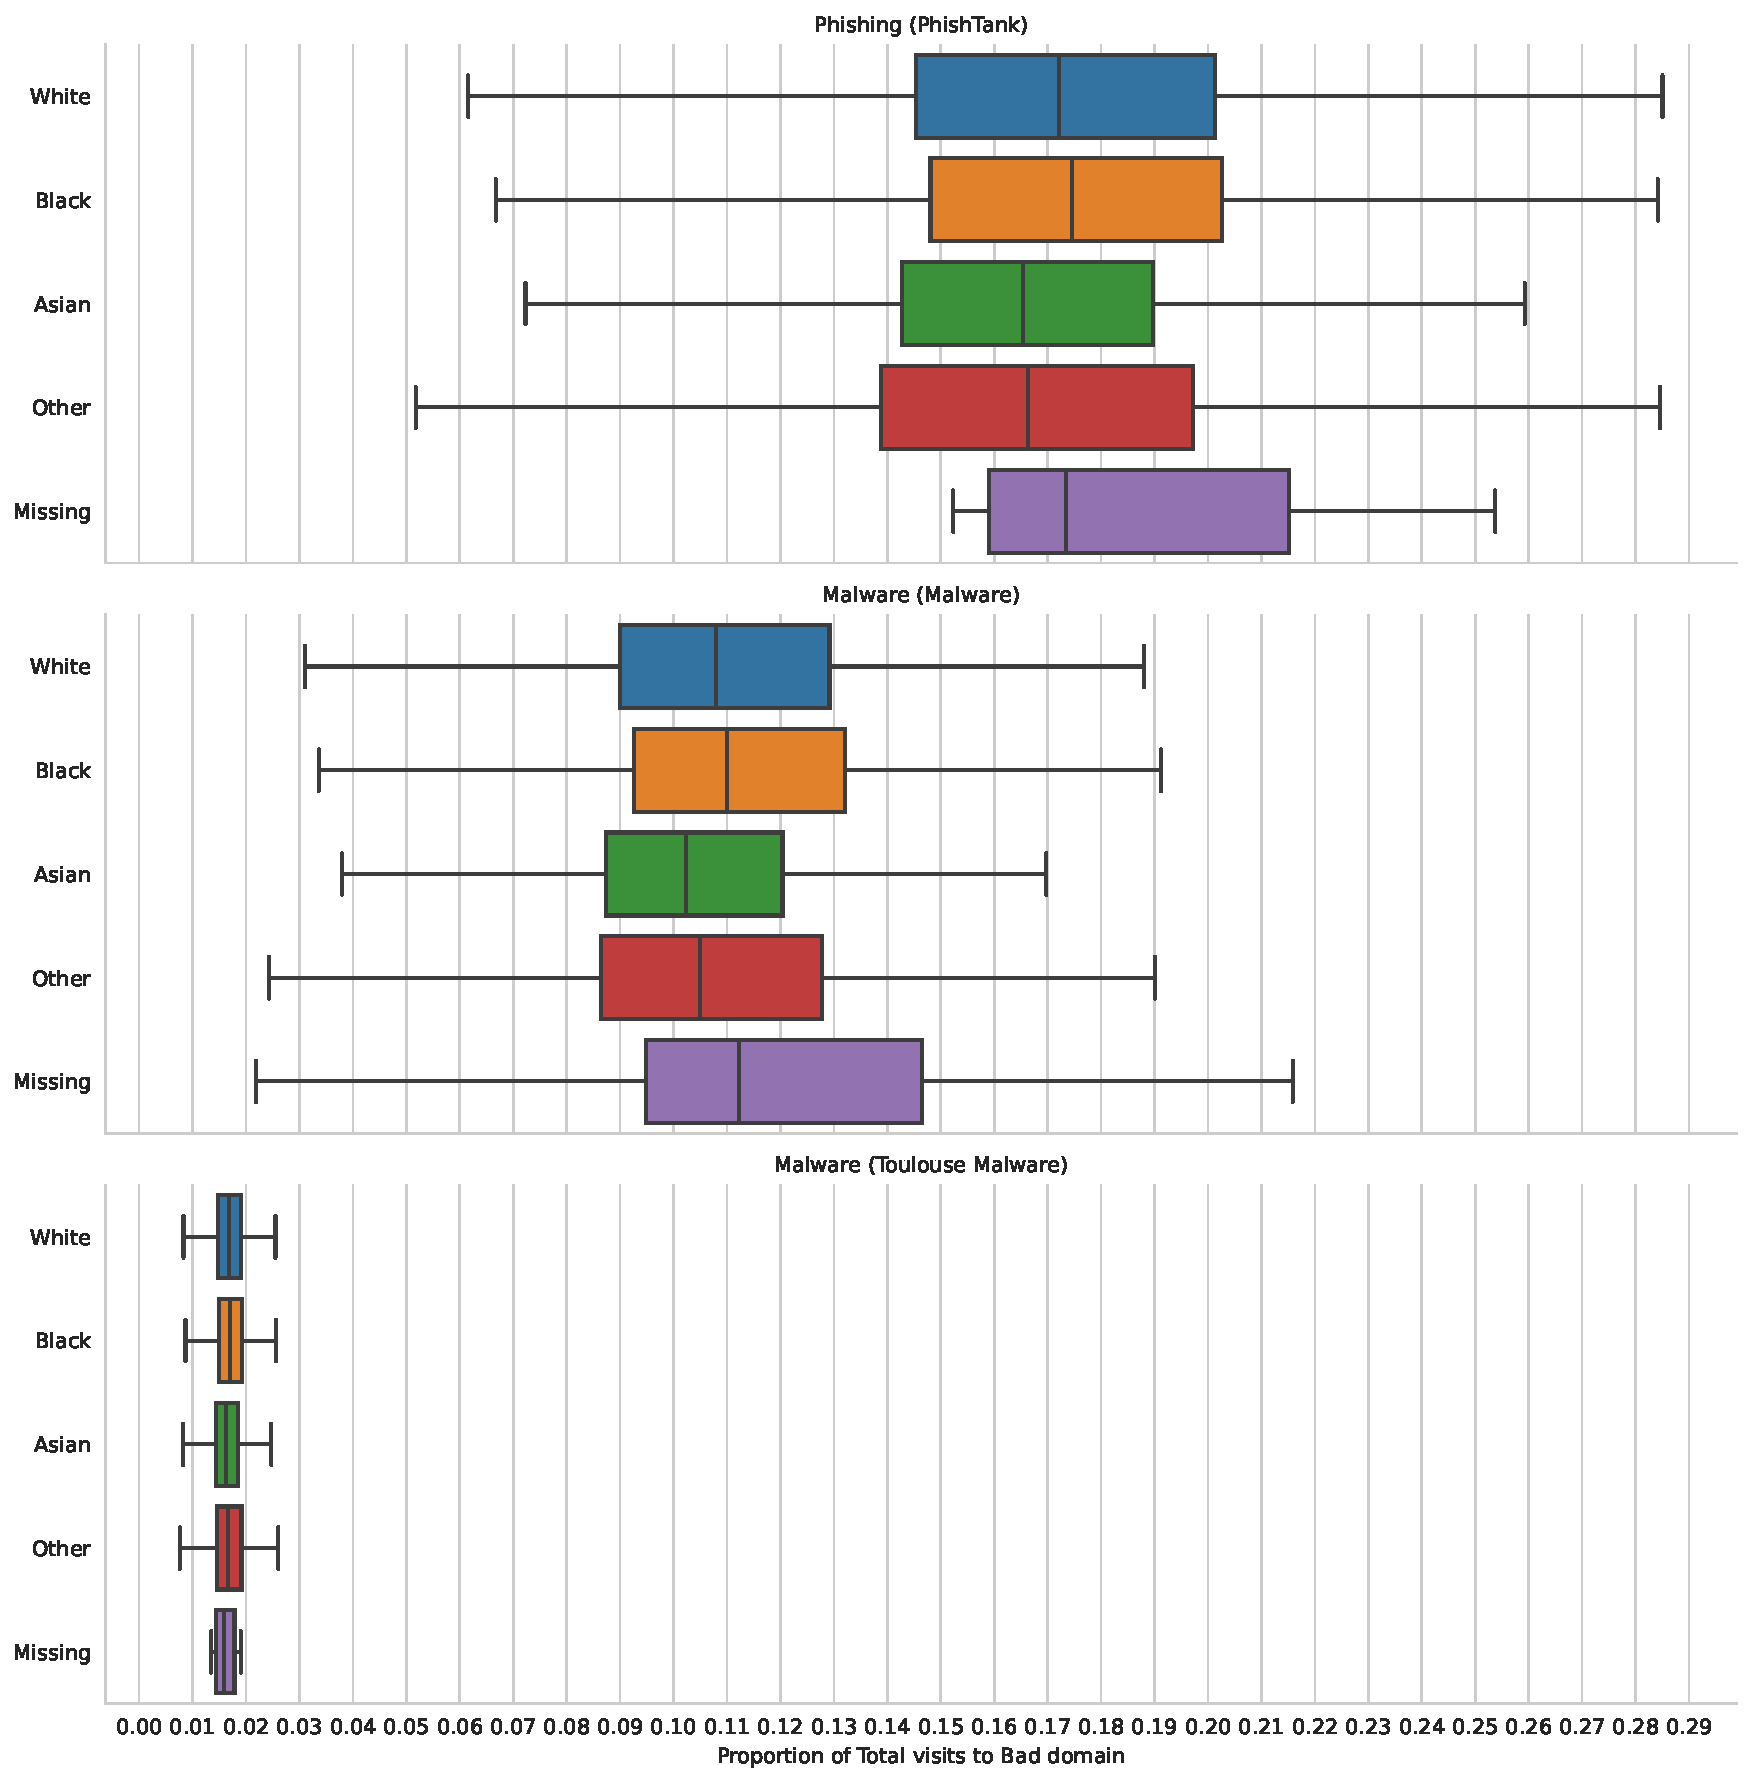
\includegraphics[width=\textwidth]{figs/prop_total_visits_phishing_malware_tl_race.pdf}
	\end{figure}

\begin{figure}[!htb]
	 \centering
	 \caption{Proportion of Visits to Phishing/Malware Domains by Age}
	 \label{fig:prop_total_visits_phishing_malware_age}
	 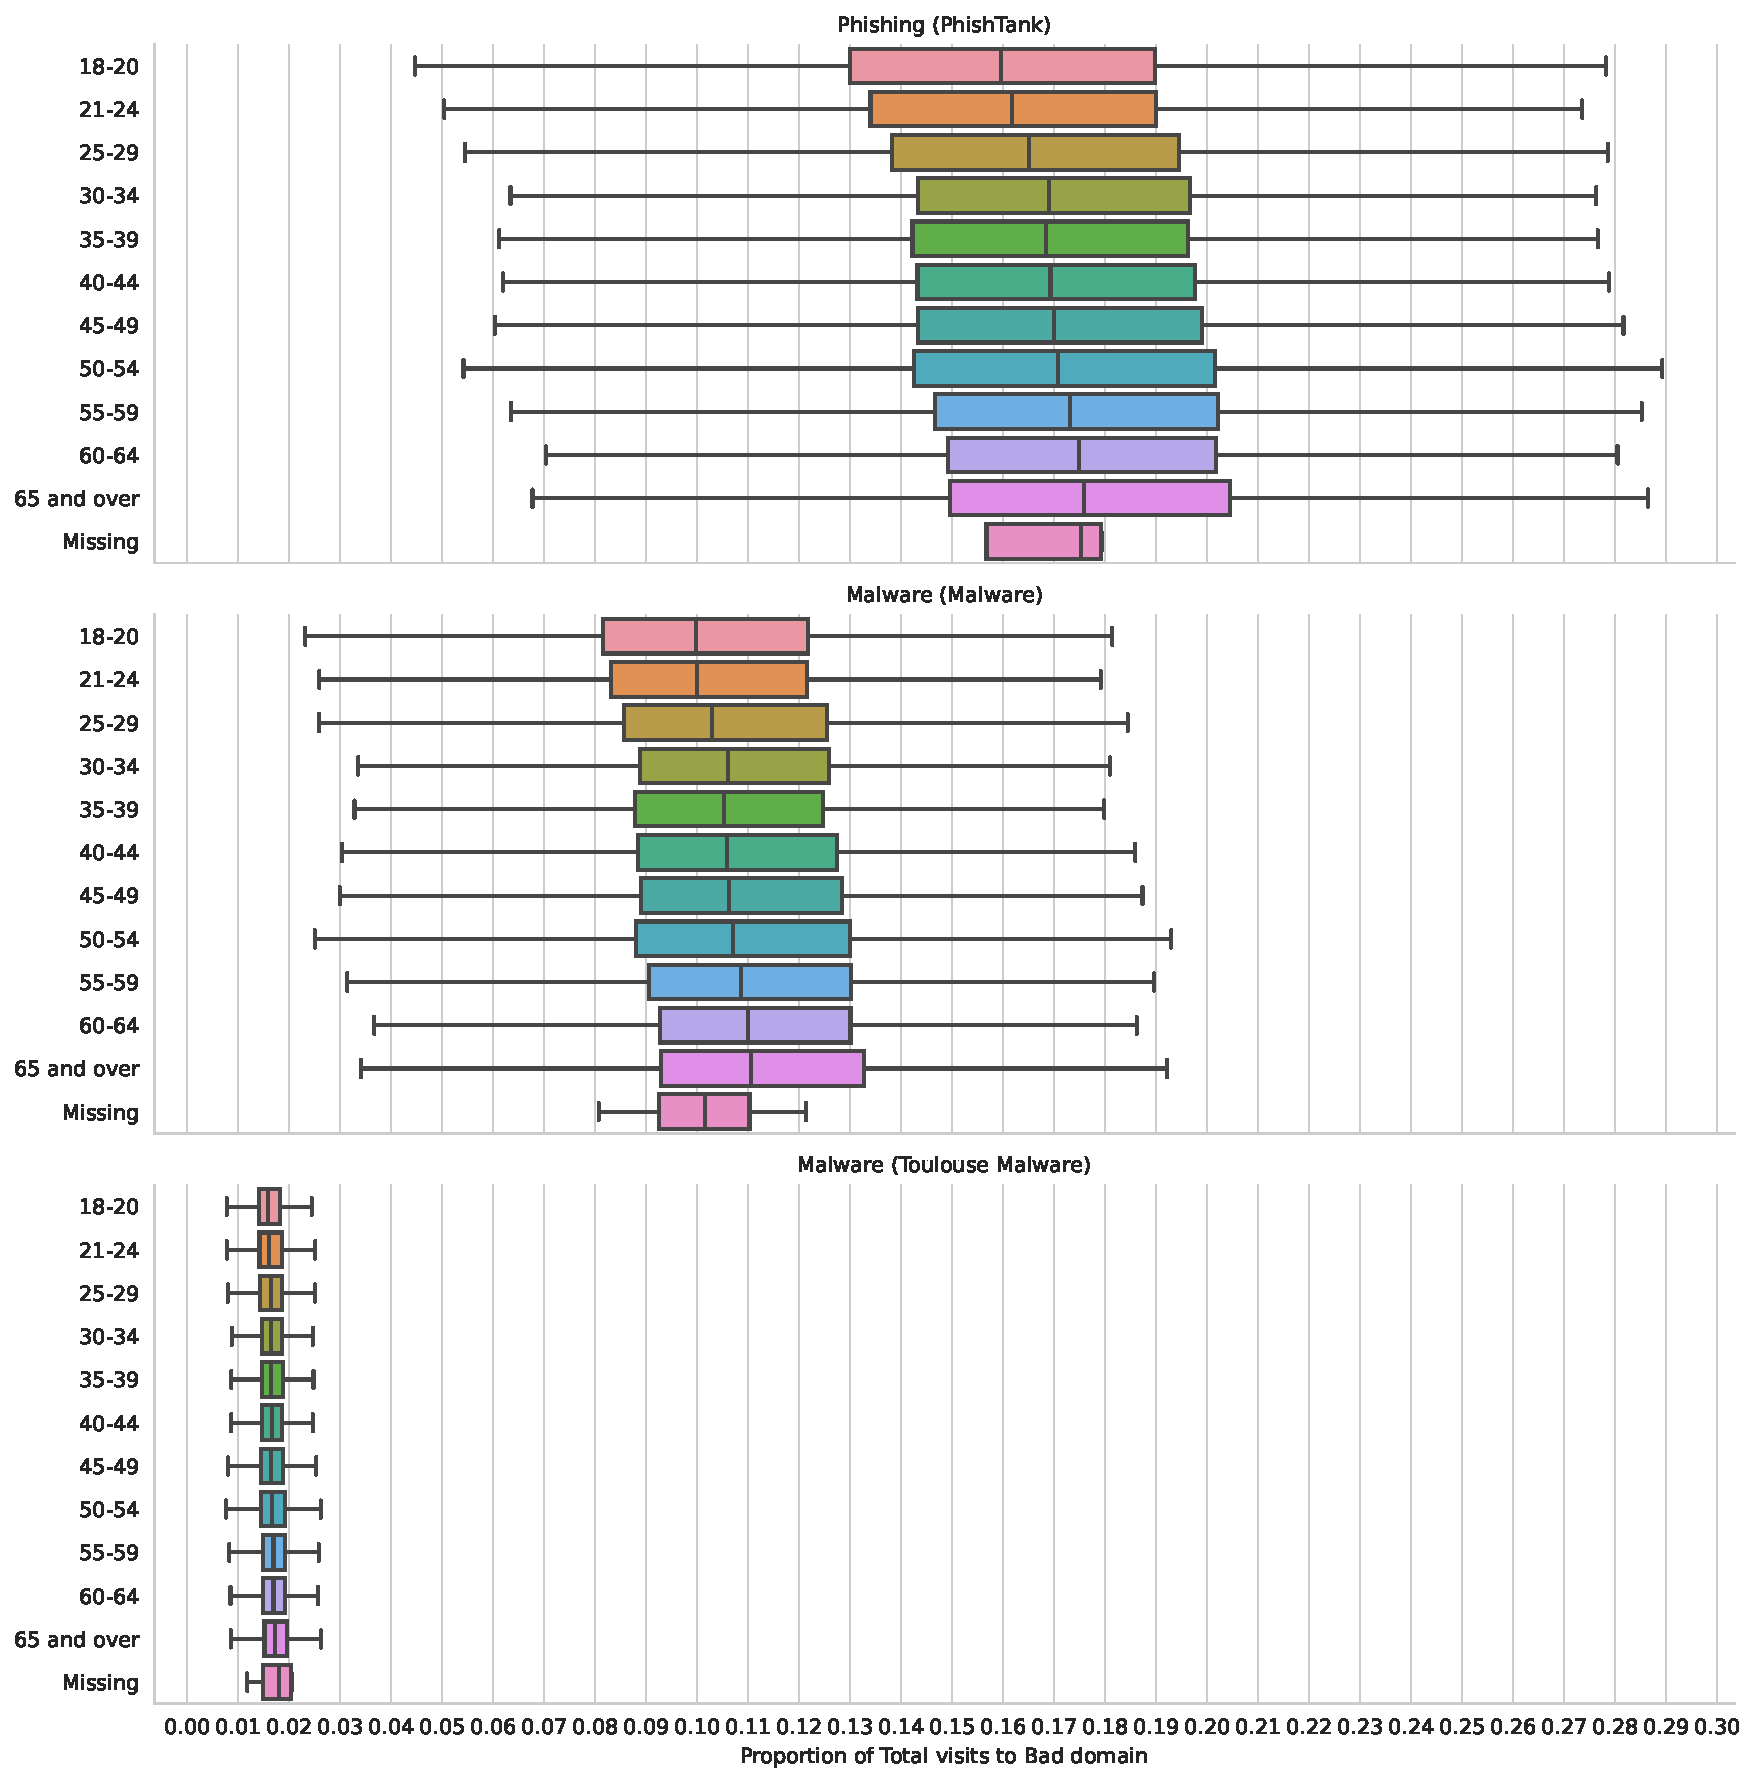
\includegraphics[width=\textwidth]{figs/prop_total_visits_phishing_malware_tl_age.pdf}
\end{figure}


\begin{figure}[!htb]
  \centering
  \caption{Proportion of Time Spent on Pornographic Domains by Education}
	\label{fig:prop_time_porn_educ}
	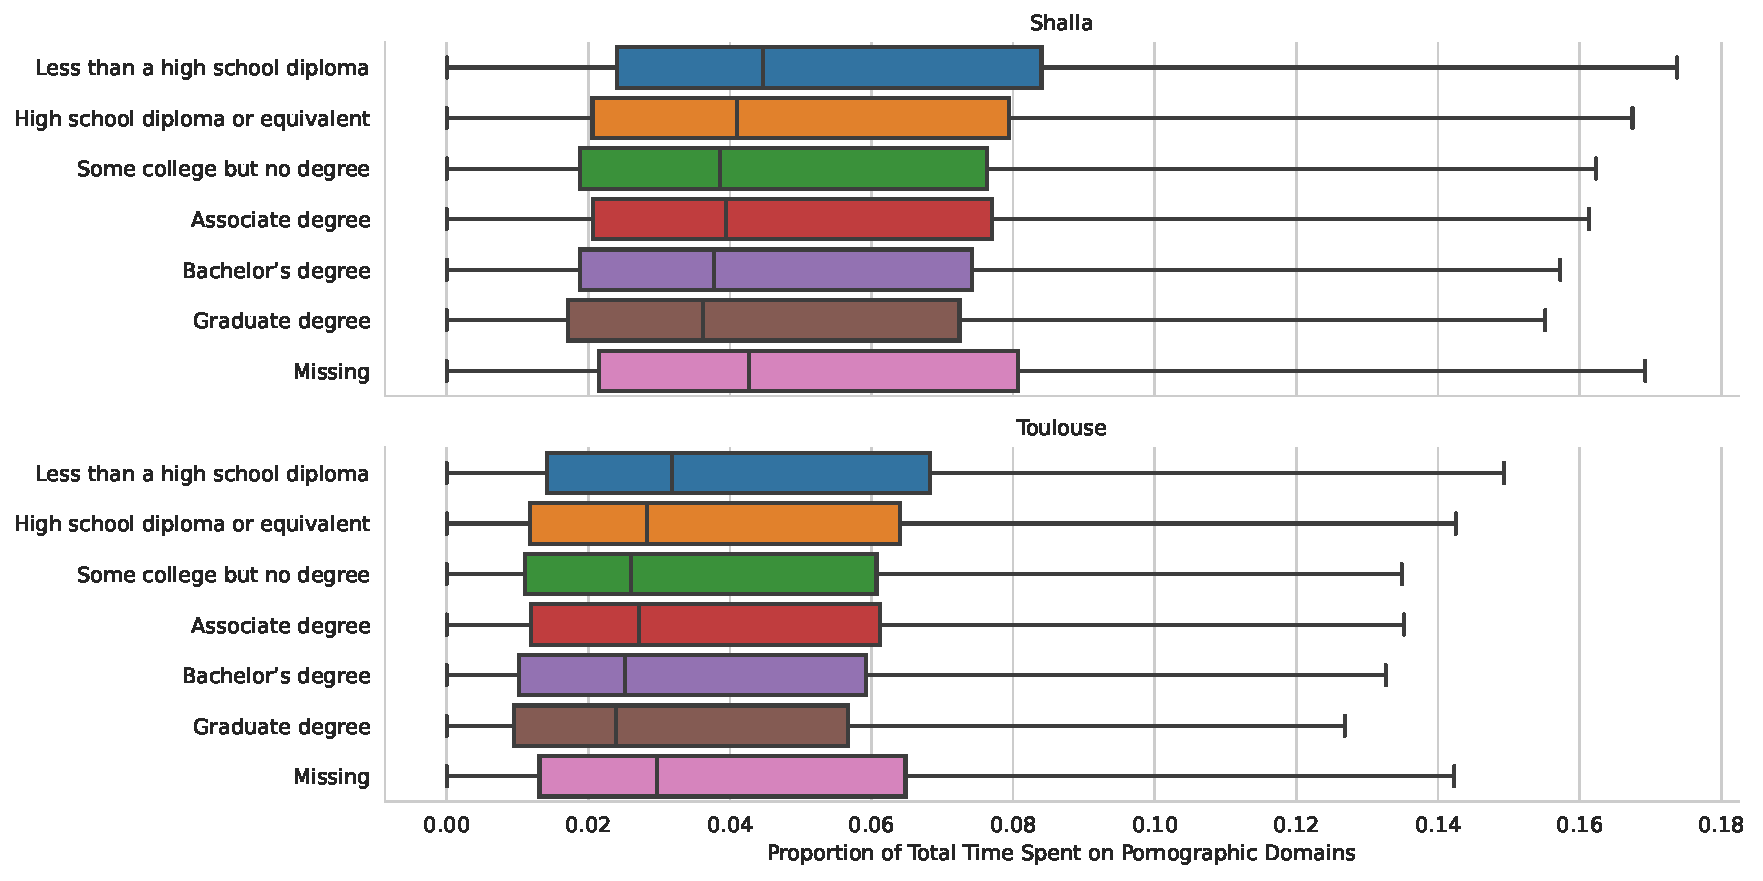
\includegraphics[width=\textwidth]{figs/prop_total_time_porn_educ.pdf}
\end{figure}

\begin{figure}[!htb]
	\centering
	\caption{Proportion of Time Spent on Pornographic Domains by Age}
	\label{fig:prop_time_porn_age}
	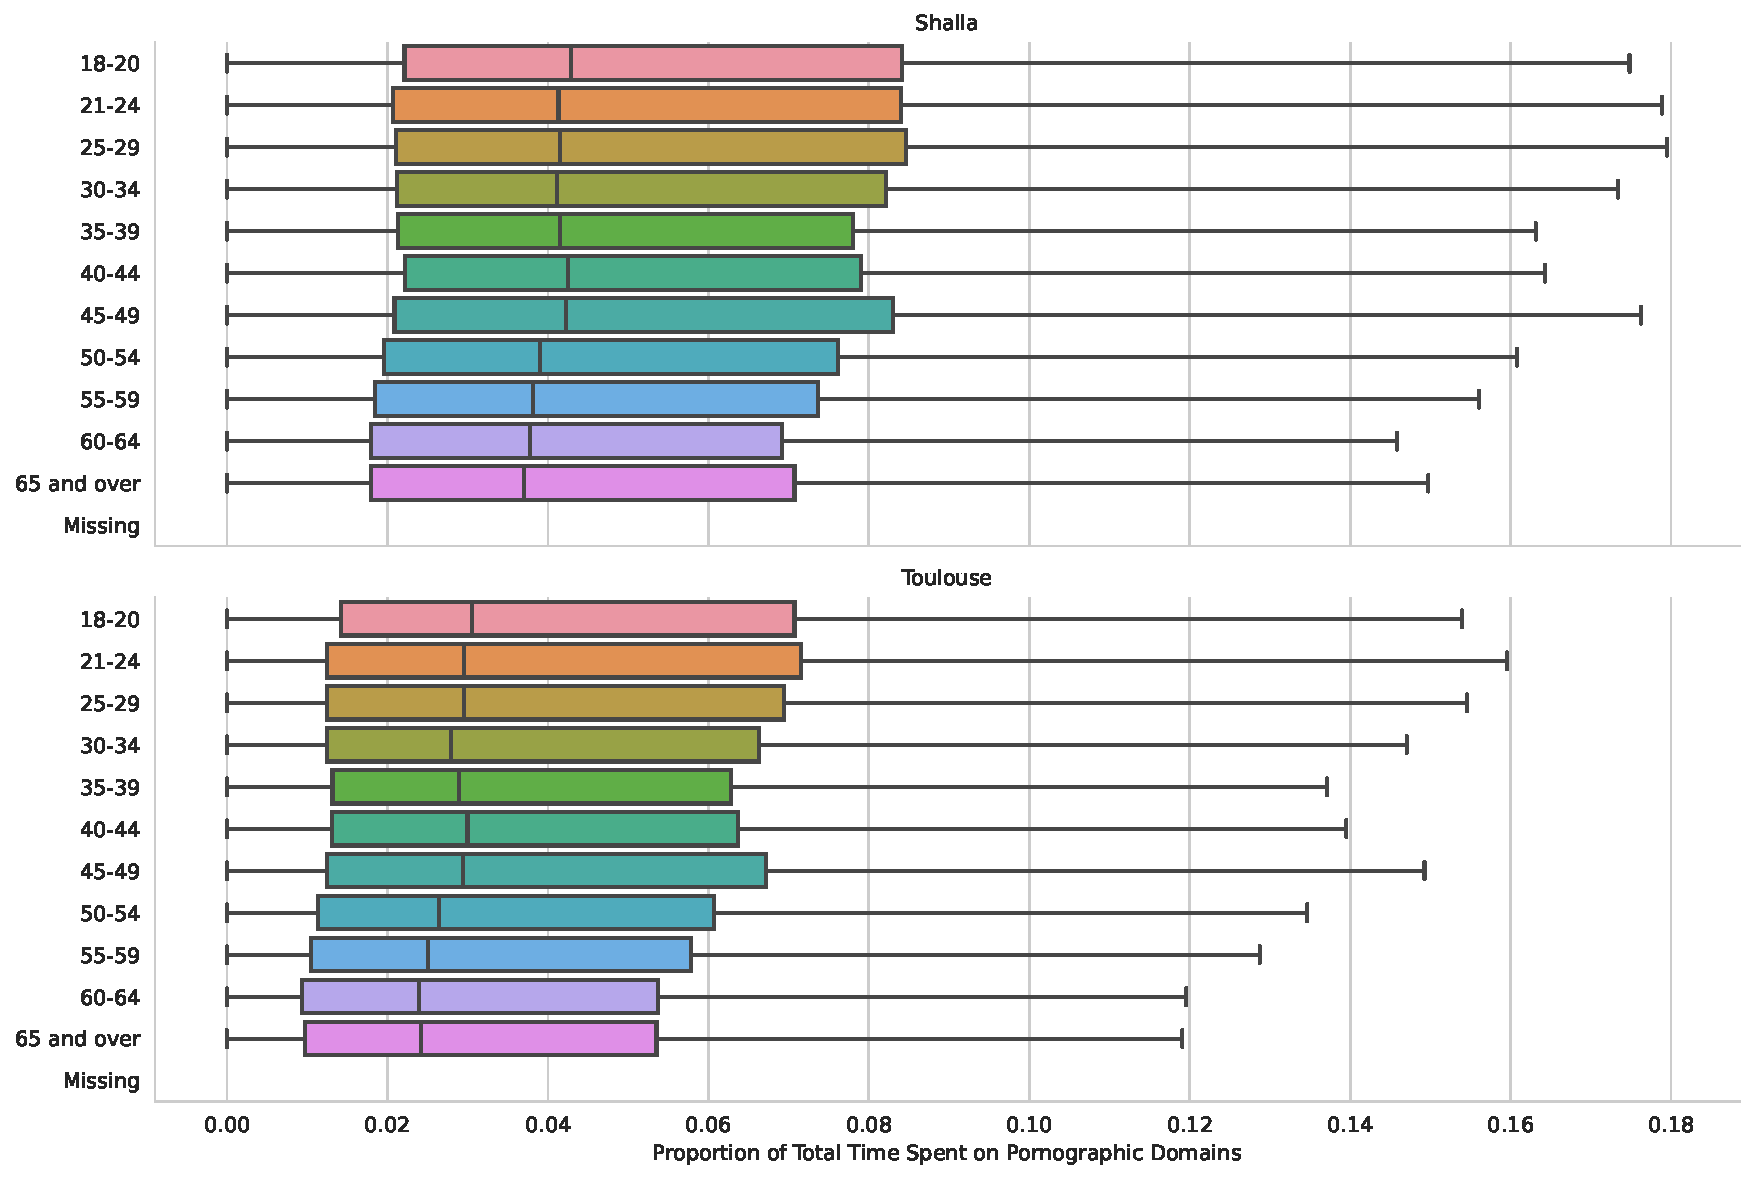
\includegraphics[width=\textwidth]{figs/prop_total_time_porn_age.pdf}
\end{figure}

\end{document}
